
            \documentclass[10pt,a4paper]{article}
            \usepackage[latin1]{inputenc}
            \usepackage[T1]{fontenc}
            \usepackage{amsmath}
            \usepackage{amsfonts}
            \usepackage{amssymb}
            \usepackage{graphicx}
            \usepackage{caption}
            \usepackage{lmodern}
            \usepackage{placeins}
            \usepackage{multicol}
            \usepackage{tikz}
            \usetikzlibrary{shapes.arrows,chains, positioning}
            \usepackage{booktabs} %professional tables
            \usepackage[left=2cm,right=2cm,top=2cm,bottom=2cm]{geometry}
            \usepackage{microtype} %optimises spacing, needs to go after fonts
            \usepackage{hyperref} %adds links (also in TOC), should be loaded at the very end
            \usepackage{longtable}
            \usepackage{color}
            \usepackage{listings}

            \definecolor{gray}{rgb}{0.4,0.4,0.4}
            \definecolor{darkblue}{rgb}{0.0,0.0,0.6}
            \definecolor{cyan}{rgb}{0.0,0.6,0.6}

            \lstset{
              basicstyle=\ttfamily\scriptsize,
              columns=fullflexible,
              showstringspaces=false,
              commentstyle=\color{gray}\upshape
            }

            \lstdefinelanguage{XML}
            {
              morestring=[b]",
              morestring=[s]{>}{<},
              morecomment=[s]{<?}{?>},
              stringstyle=\color{black},
              identifierstyle=\color{darkblue},
              keywordstyle=\color{cyan},
              morekeywords={xmlns,version,type}% list your attributes here
            }

            \usepackage[load-configurations=abbreviations]{siunitx}
            \makeatletter
            % In newer versions of latex there is a problem with the calc package and tikz
            % http://tex.stackexchange.com/questions/289551/how-to-resolve-conflict-between-versions-of-texlive-and-pgf
            \def\pgfmathparse@#1{%
                % Stuff for calc compatiability.
                \let\real=\pgfmath@calc@real
                \let\minof=\pgfmath@calc@minof
                \let\maxof=\pgfmath@calc@maxof
                \let\ratio=\pgfmath@calc@ratio
                \let\widthof=\pgfmath@calc@widthof
                \let\heightof=\pgfmath@calc@heightof
                \let\depthof=\pgfmath@calc@depthof
                % No (math) units yet.
                \global\pgfmathunitsdeclaredfalse
                \global\pgfmathmathunitsdeclaredfalse
                % Expand expression so any reamining CSs are registers
                % or box dimensions (i.e. |\wd|, |\ht|, |\dp|).
                \edef\pgfmath@expression{#1}%
                    %
                    \expandafter\pgfmathparse@trynumber@loop\pgfmath@expression\pgfmath@parse@stop
                    %
                    % this here is the _real_ parser. it is invoked by
                    % \pgfmathparse@trynumber@loop if that says "this is no number"
                    %\pgfmathparse@@\pgfmath@parse@stop%
                }
            \makeatother
            \begin{document}
            \author{Thomas Keck\\ Moritz Gelb\\ Nils Braun\\}
\date{\today}
\title{Automatic MVA Evaluation}
\maketitle
\begin{abstract}
Evaluation plots
\end{abstract}
\clearpage
\tableofcontents
\FloatBarrier
\clearpage
\raggedbottom
\pagebreak[0]
\FloatBarrier
\section{Classifiers}

            This section contains the GeneralOptions and SpecificOptions of all classifiers represented by an XML tree.
            The same information can be retrieved using the basf2\_mva\_info tool.
        \begin{center}
\begin{longtable}{ll}
\caption{Abbreviations of identifiers}\\
\toprule
Identifier & Abbreviation\\
\midrule
/home/belle2/ssana/MC15ri\_cs1/cs/test/MVAFastBDT.root & /home\\
\bottomrule
\end{longtable}
\end{center}
\subsection{/home/belle2/ssana/MC15ri\_cs1/cs/test/MVAFastBDT.root}
\lstset{language=XML}
\begin{lstlisting}[breaklines=true]
<?xml version="1.0" encoding="utf-8"?>
<method>FastBDT</method>
<weightfile>/home/belle2/ssana/MC15ri_cs1/cs/test/MVAFastBDT.root</weightfile>
<treename>tree</treename>
<target_variable>isSignal</target_variable>
<weight_variable>__weight__</weight_variable>
<signal_class>1</signal_class>
<max_events>0</max_events>
<number_feature_variables>17</number_feature_variables>
<variable0>abs_qr</variable0>
<variable1>DeltaZ</variable1>
<variable2>R2</variable2>
<variable3>thrustBm</variable3>
<variable4>thrustOm</variable4>
<variable5>cosTBTO</variable5>
<variable6>cosTBz</variable6>
<variable7>CMS_cosTheta</variable7>
<variable8>KSFWVariables(et)</variable8>
<variable9>KSFWVariables(hso01)</variable9>
<variable10>KSFWVariables(hso02)</variable10>
<variable11>KSFWVariables(hso10)</variable11>
<variable12>KSFWVariables(hso12)</variable12>
<variable13>KSFWVariables(hso20)</variable13>
<variable14>KSFWVariables(hoo0)</variable14>
<variable15>CleoConeCS(1)</variable15>
<variable16>CleoConeCS(2)</variable16>
<number_spectator_variables>0</number_spectator_variables>
<number_data_files>1</number_data_files>
<datafile0>/home/belle2/ssana/MC15ri_cs1/cs/train/signal_scaled/train.root</datafile0>
<FastBDT_version>2</FastBDT_version>
<FastBDT_nTrees>200</FastBDT_nTrees>
<FastBDT_nCuts>8</FastBDT_nCuts>
<FastBDT_nLevels>3</FastBDT_nLevels>
<FastBDT_shrinkage>0.10000000000000001</FastBDT_shrinkage>
<FastBDT_randRatio>0.5</FastBDT_randRatio>
<FastBDT_flatnessLoss>-1</FastBDT_flatnessLoss>
<FastBDT_sPlot>false</FastBDT_sPlot>
<FastBDT_number_individual_nCuts>0</FastBDT_number_individual_nCuts>
<FastBDT_purityTransformation>false</FastBDT_purityTransformation>
<FastBDT_number_individualPurityTransformation>0</FastBDT_number_individualPurityTransformation>
\end{lstlisting}\raggedbottom
\pagebreak[0]
\FloatBarrier
\section{Variables}

            This section contains an overview of the importance and correlation of the variables used by the classifiers.
            And distribution plots of the variables on the independent dataset. The distributions are normed for signal and
            background separately, and only the region +- 3 sigma around the mean is shown.
        \begin{center}
\begin{longtable}{ll}
\caption{Abbreviations of variables}\\
\toprule
Variable & Abbreviation\\
\midrule
KSFWVariables(hso01) & KSFWV1\\
KSFWVariables(hso20) & KSFWV2\\
CleoConeCS(2) & CleoC1\\
KSFWVariables(hoo0) & KSFWV3\\
thrustOm & thrus1\\
KSFWVariables(et) & KSFWV4\\
CleoConeCS(1) & CleoC2\\
cosTBz & cosTB1\\
KSFWVariables(hso10) & KSFWV5\\
KSFWVariables(hso02) & KSFWV6\\
KSFWVariables(hso12) & KSFWV7\\
CMS\_cosTheta & CMS\_c\\
thrustBm & thrus2\\
cosTBTO & cosTB2\\
abs\_qr & abs\_q\\
DeltaZ & Delta\\
R2 & R2\\
\bottomrule
\end{longtable}
\end{center}
\subsection{Importance}
\begin{center}
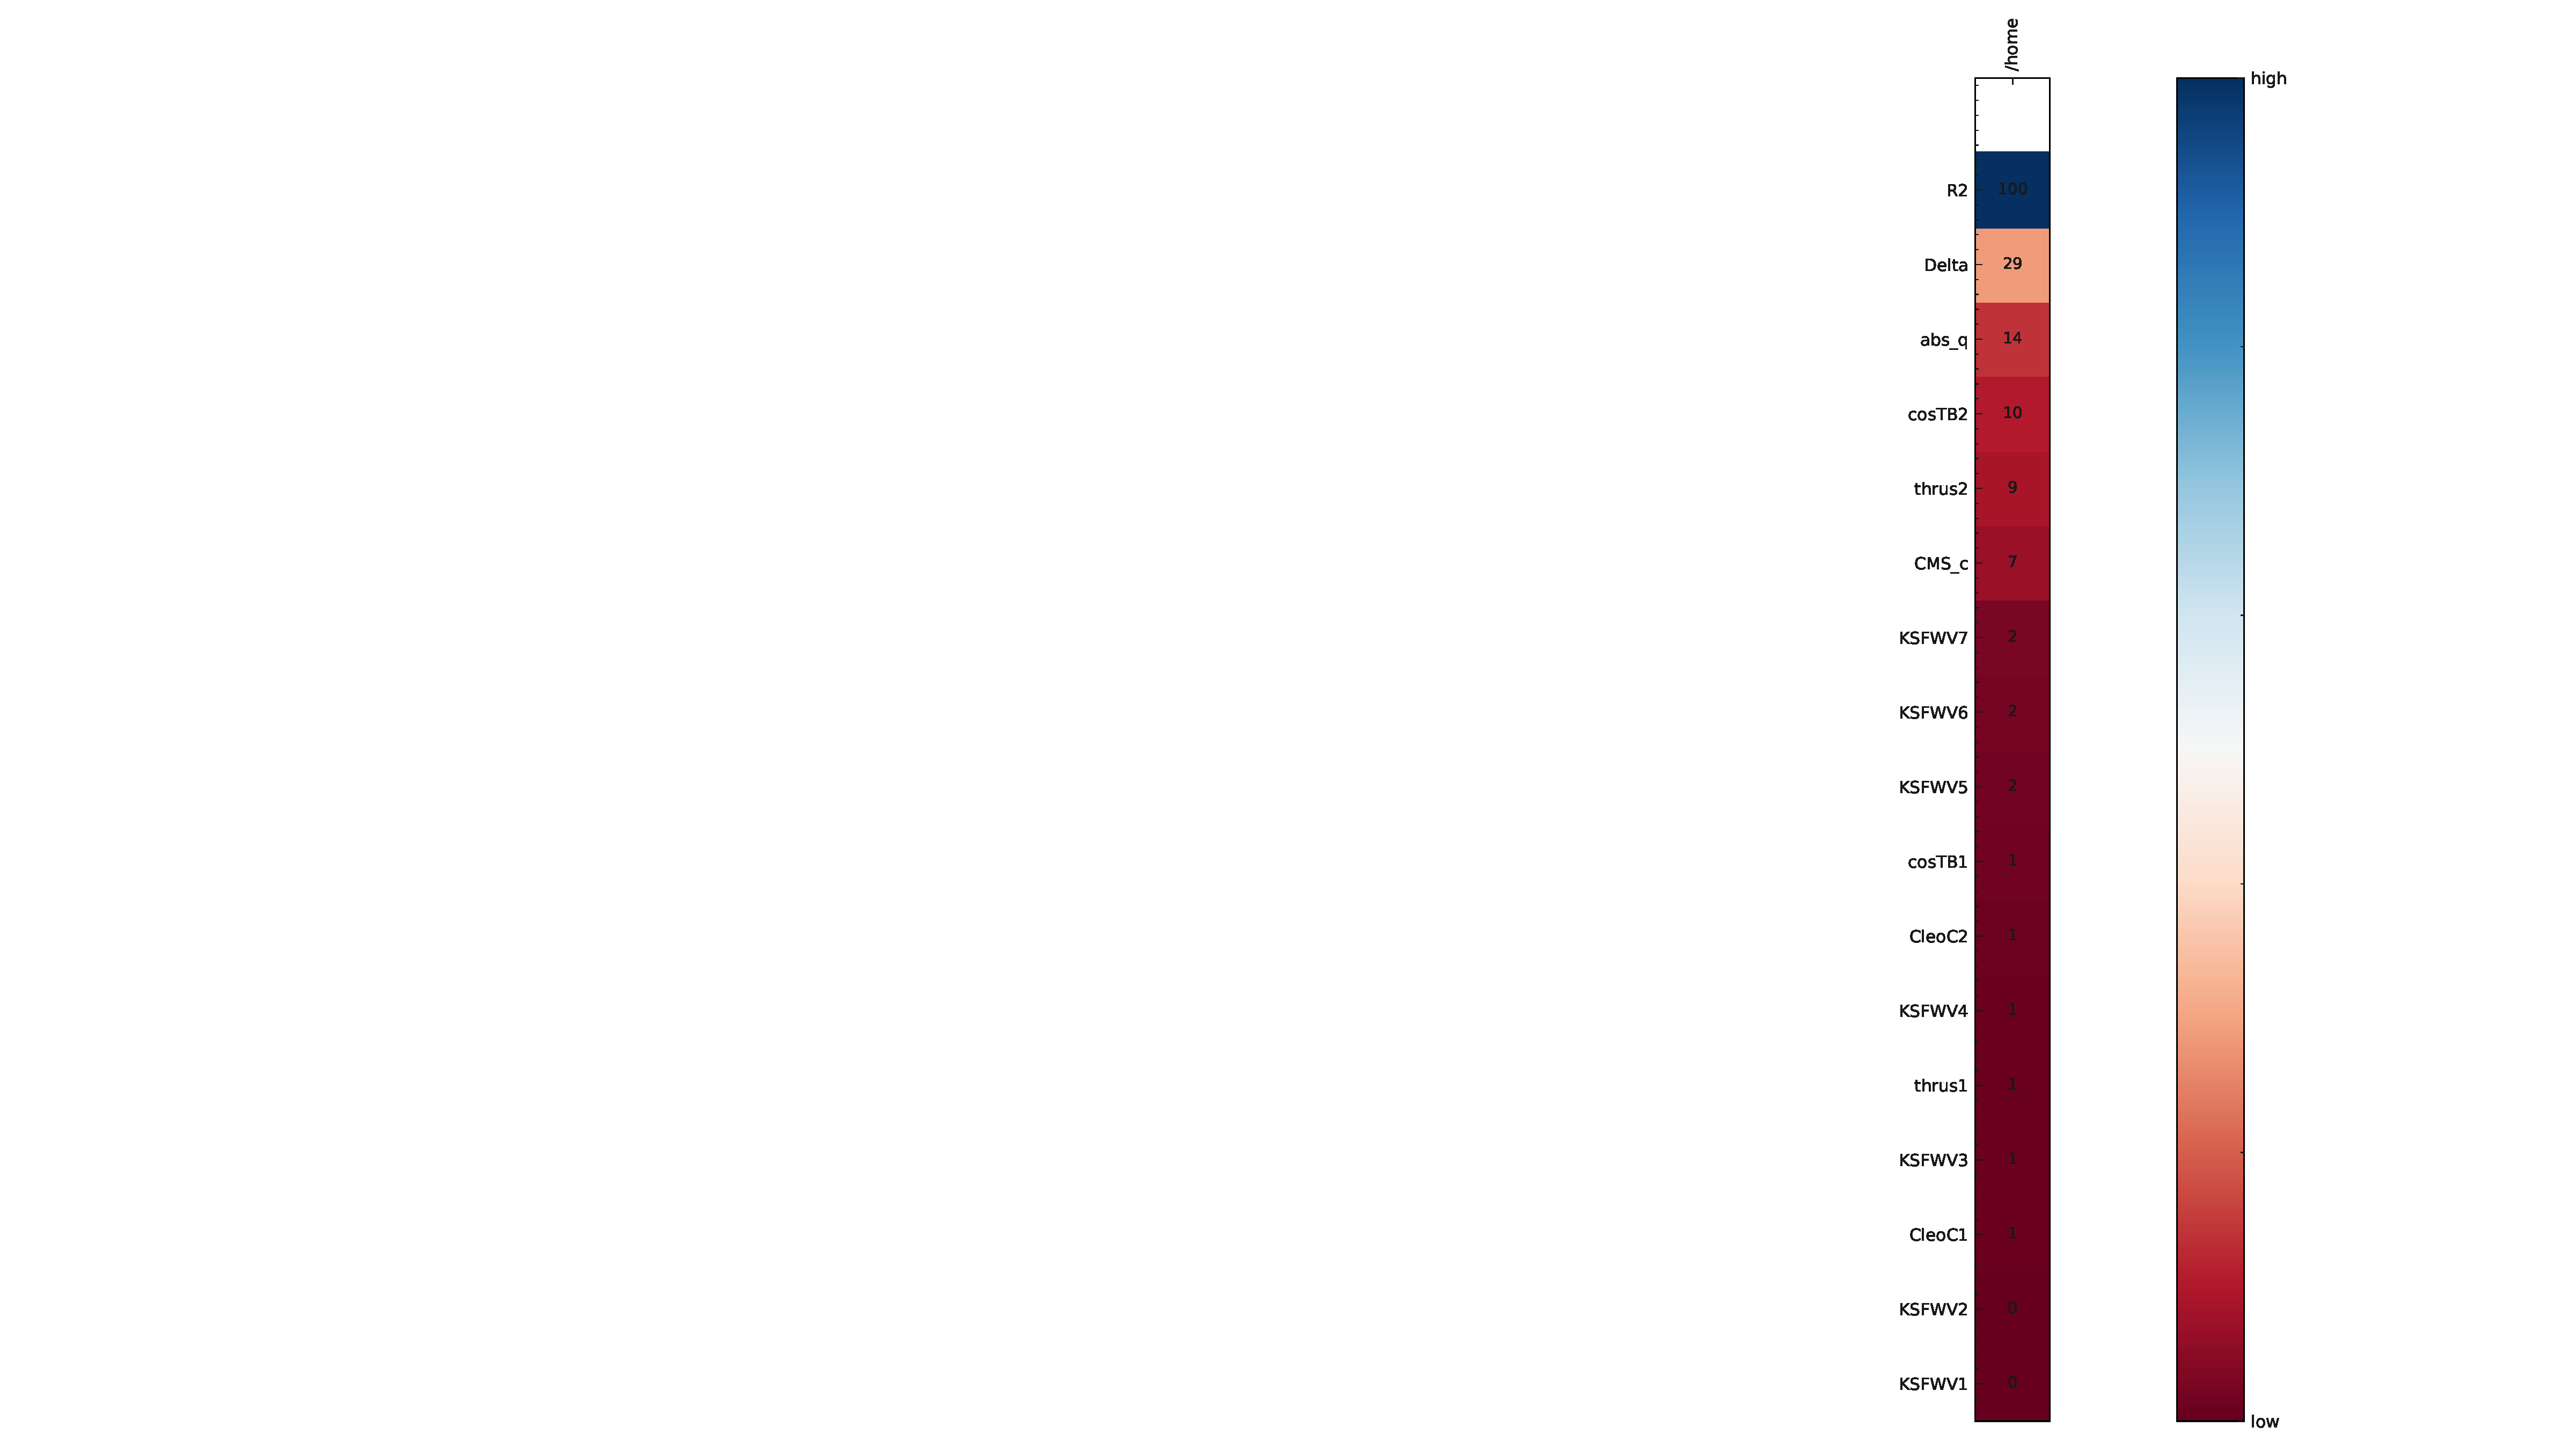
\includegraphics[width=1.0\textwidth]{importance.pdf}
\end{center}
\subsection{Correlation}
\begin{center}
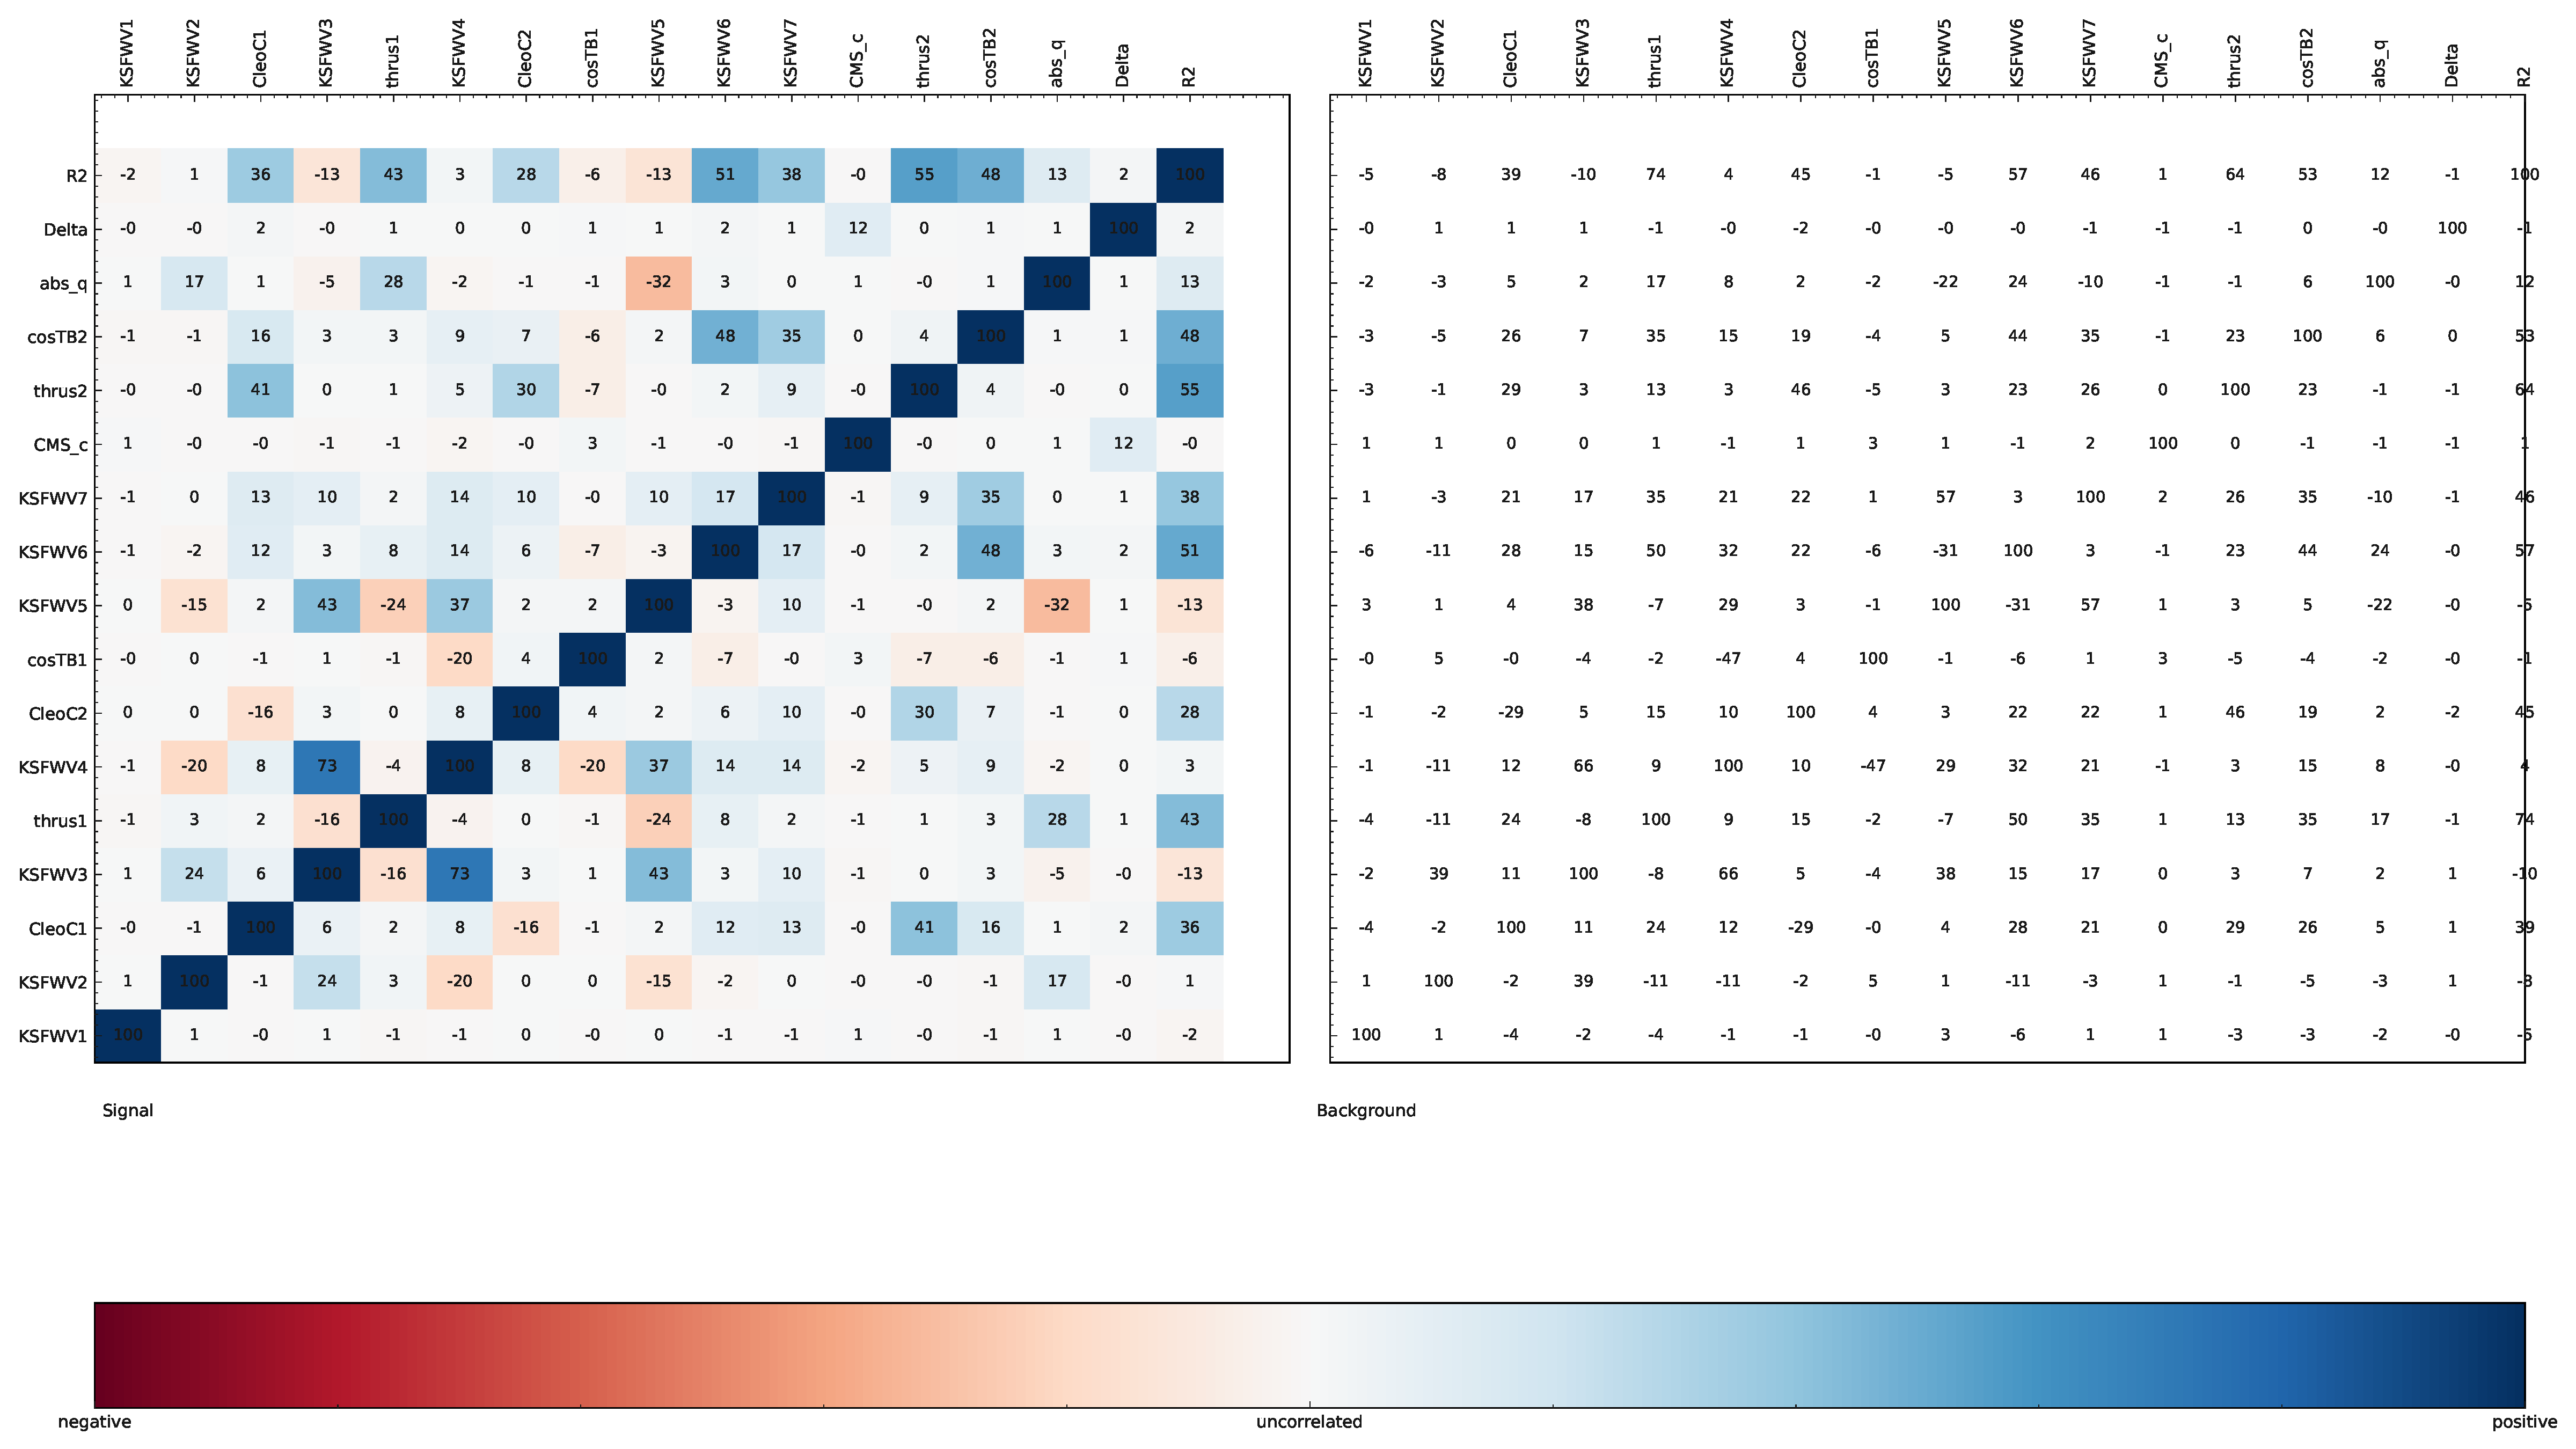
\includegraphics[width=1.0\textwidth]{correlation_plot.pdf}
\end{center}
\subsection{KSFWVariables(hso01)}
\begin{center}
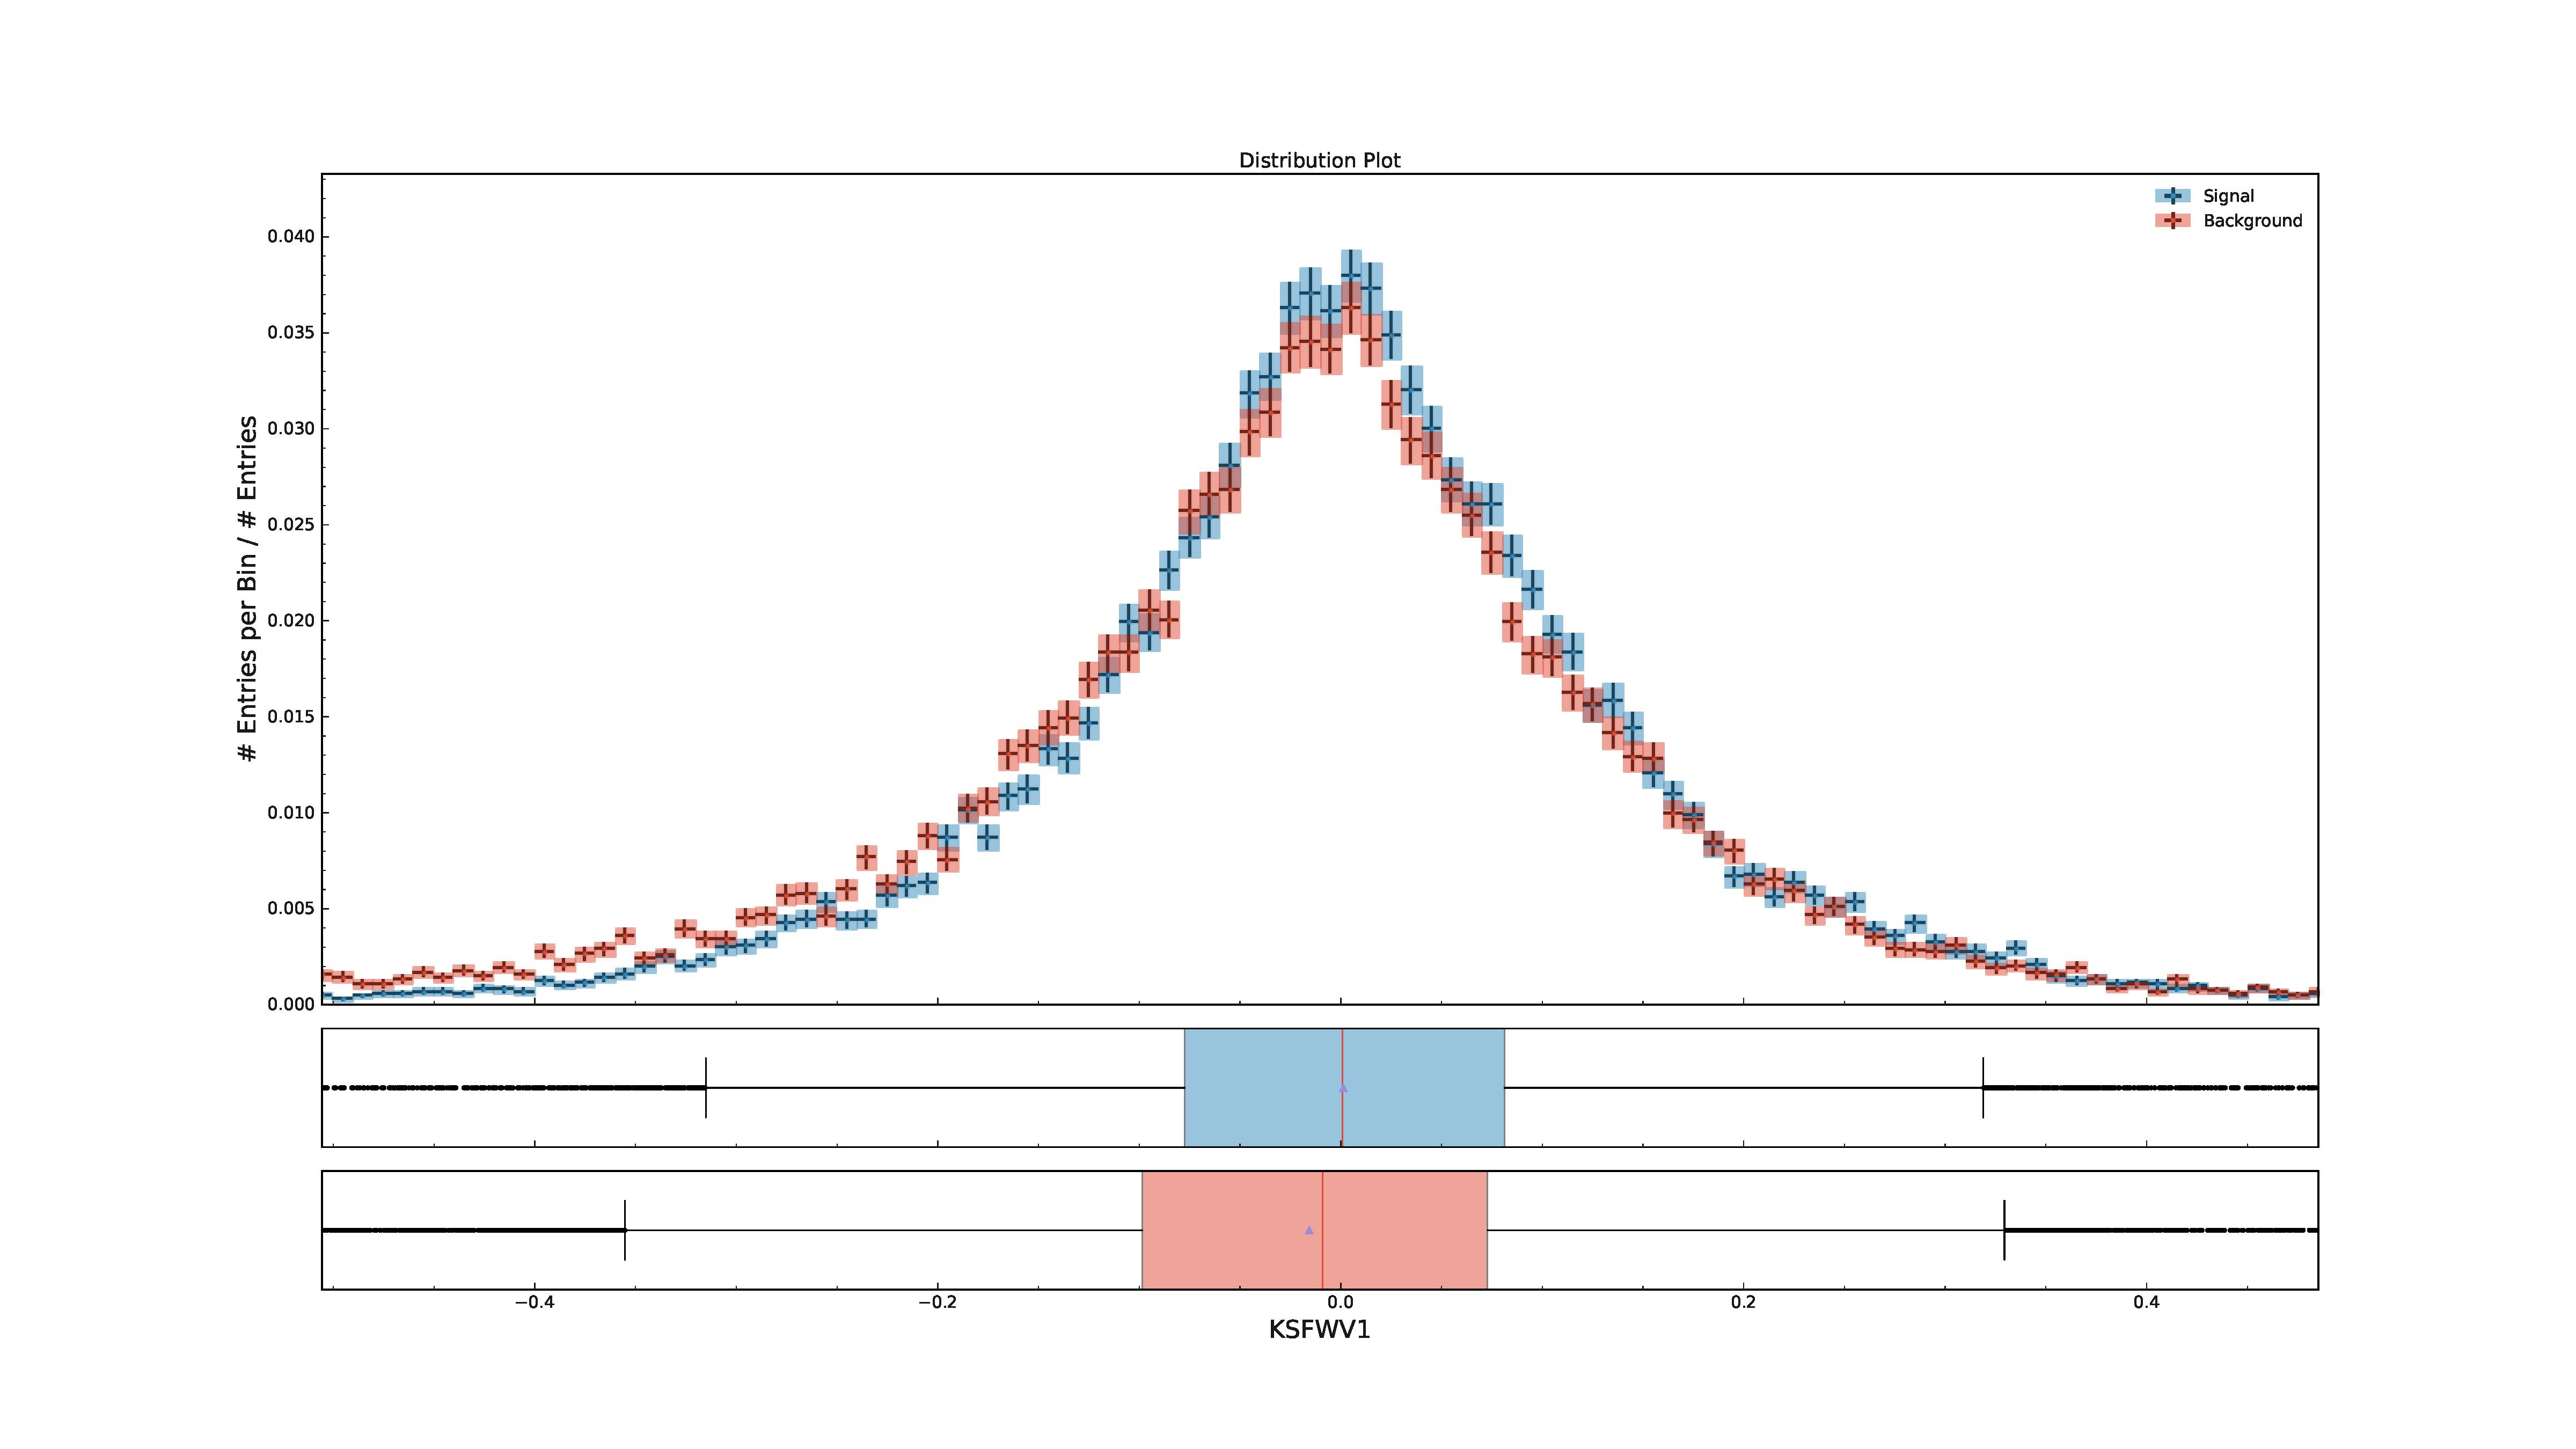
\includegraphics[width=1.0\textwidth]{variable_-6851854384329642222.pdf}
\end{center}
\subsection{KSFWVariables(hso20)}
\begin{center}
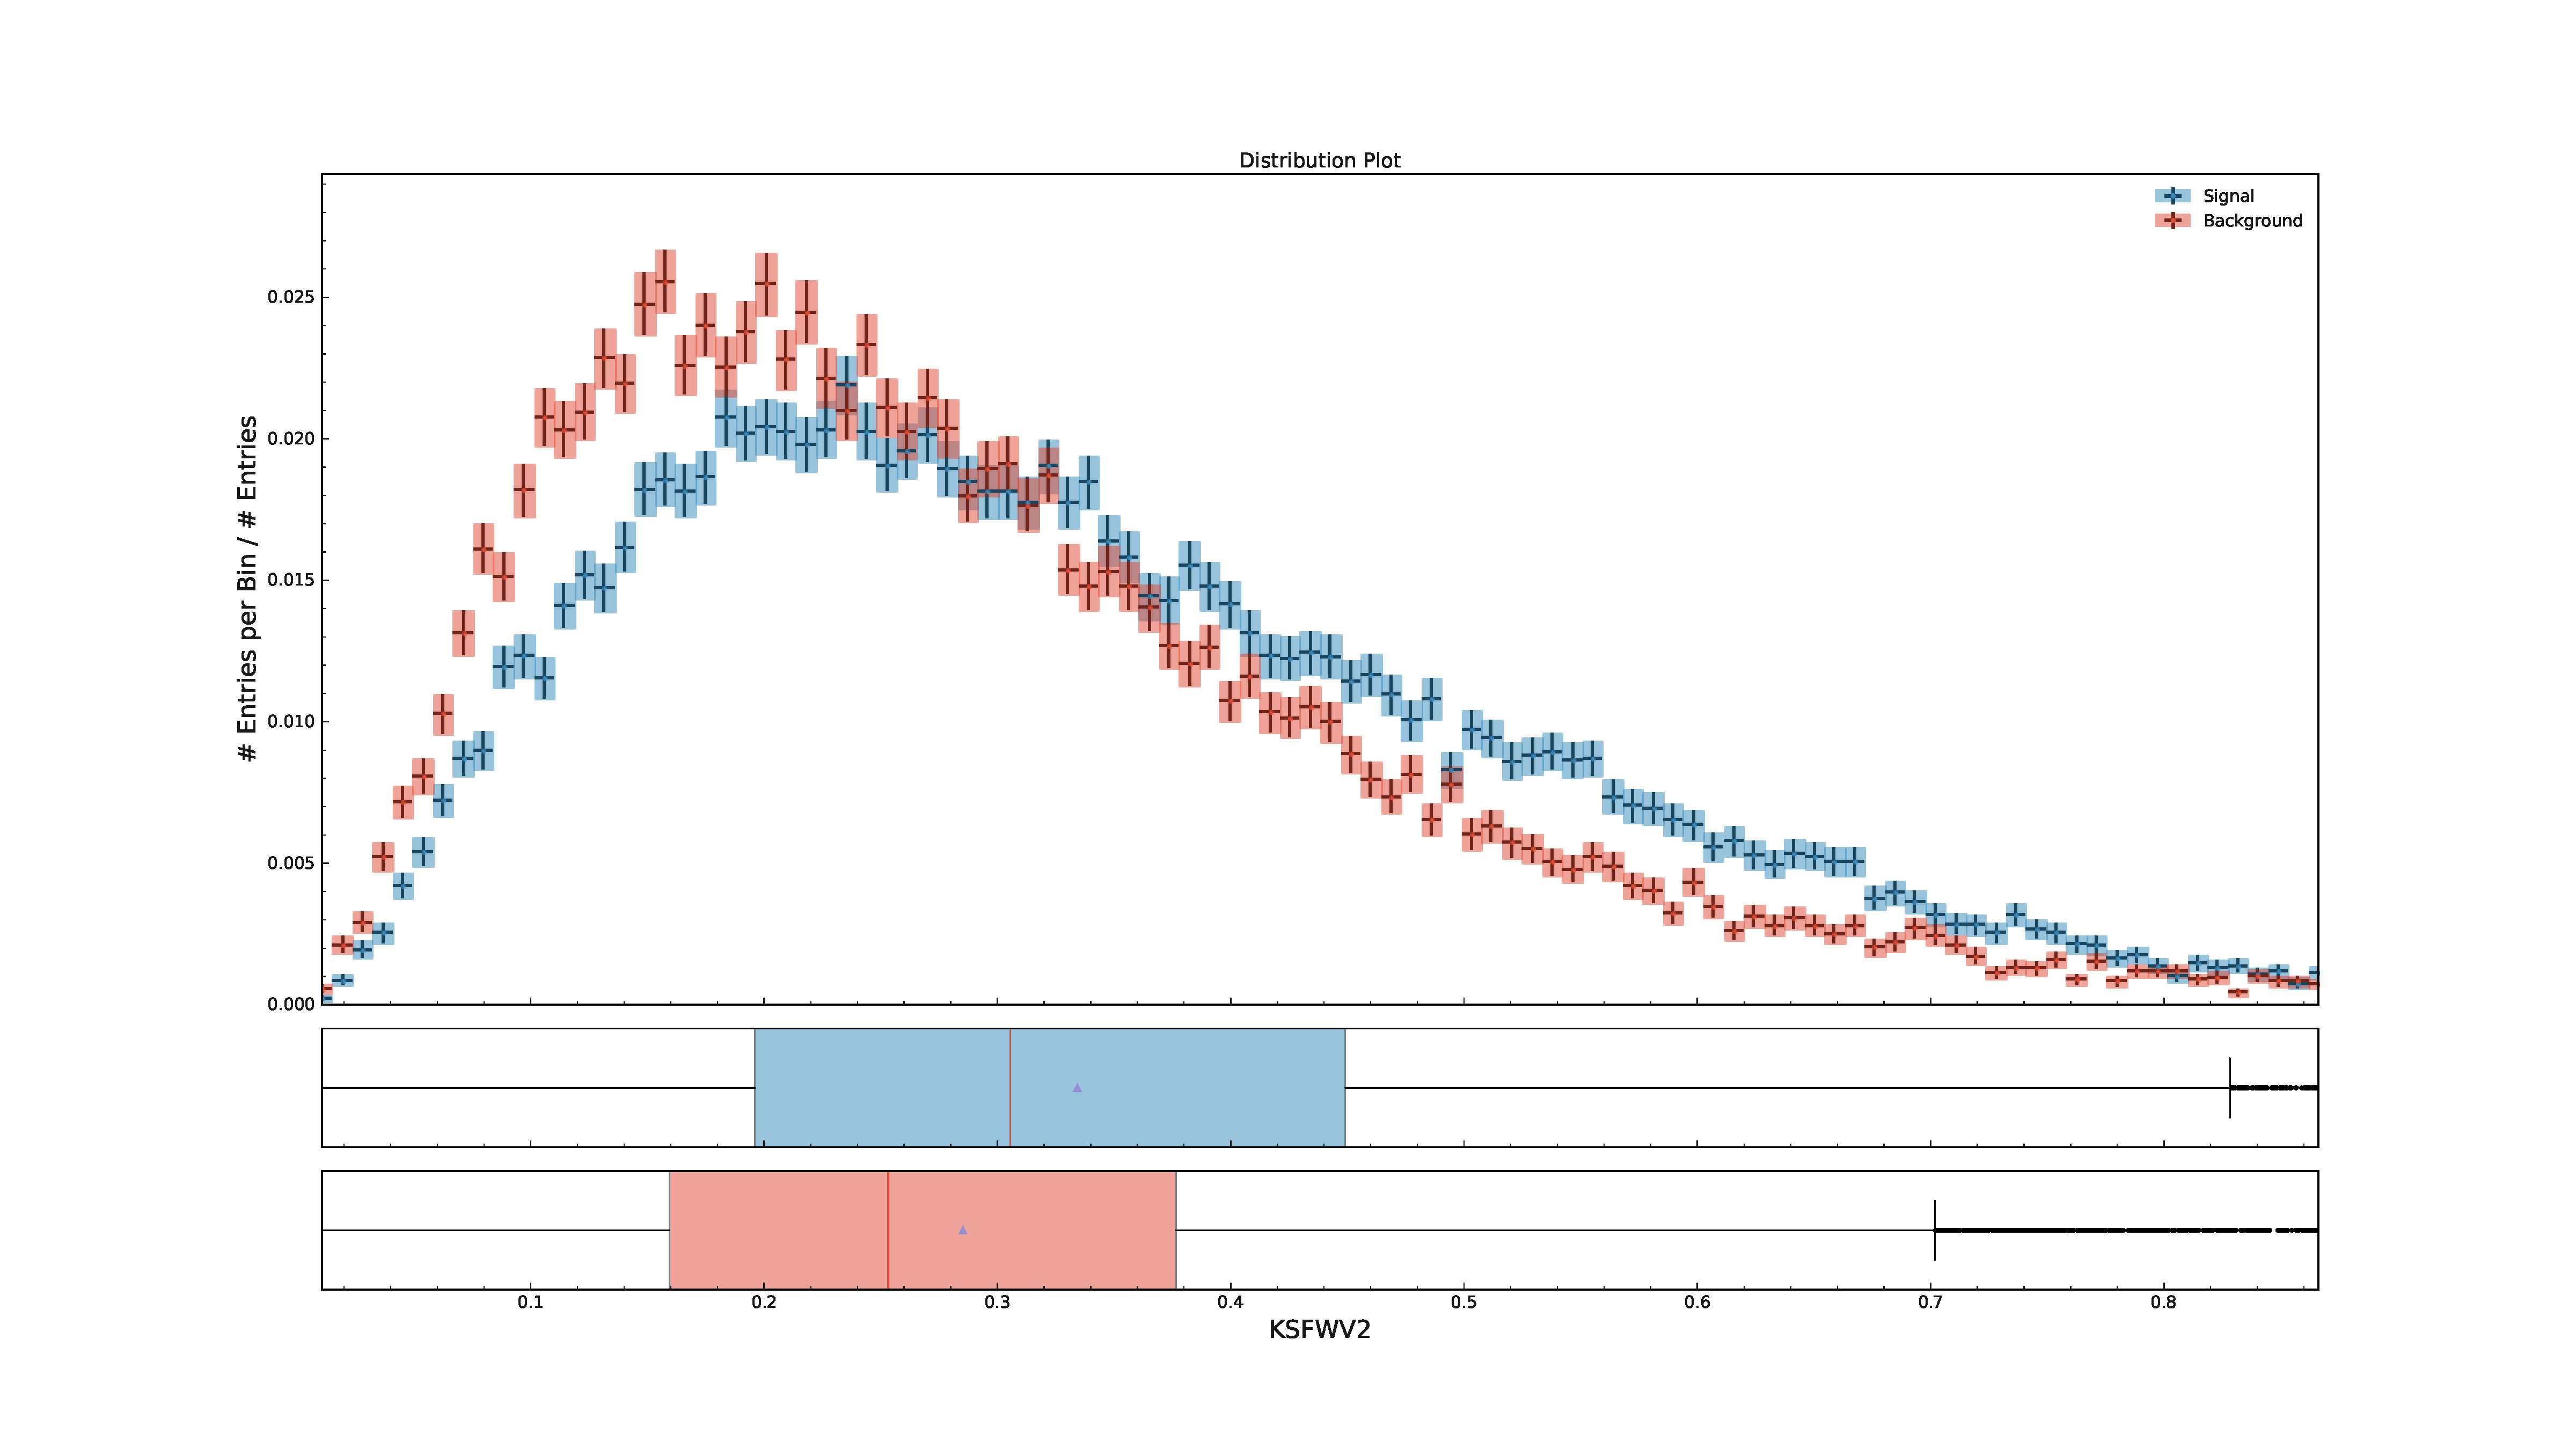
\includegraphics[width=1.0\textwidth]{variable_-7999491705771765948.pdf}
\end{center}
\subsection{CleoConeCS(2)}
\begin{center}
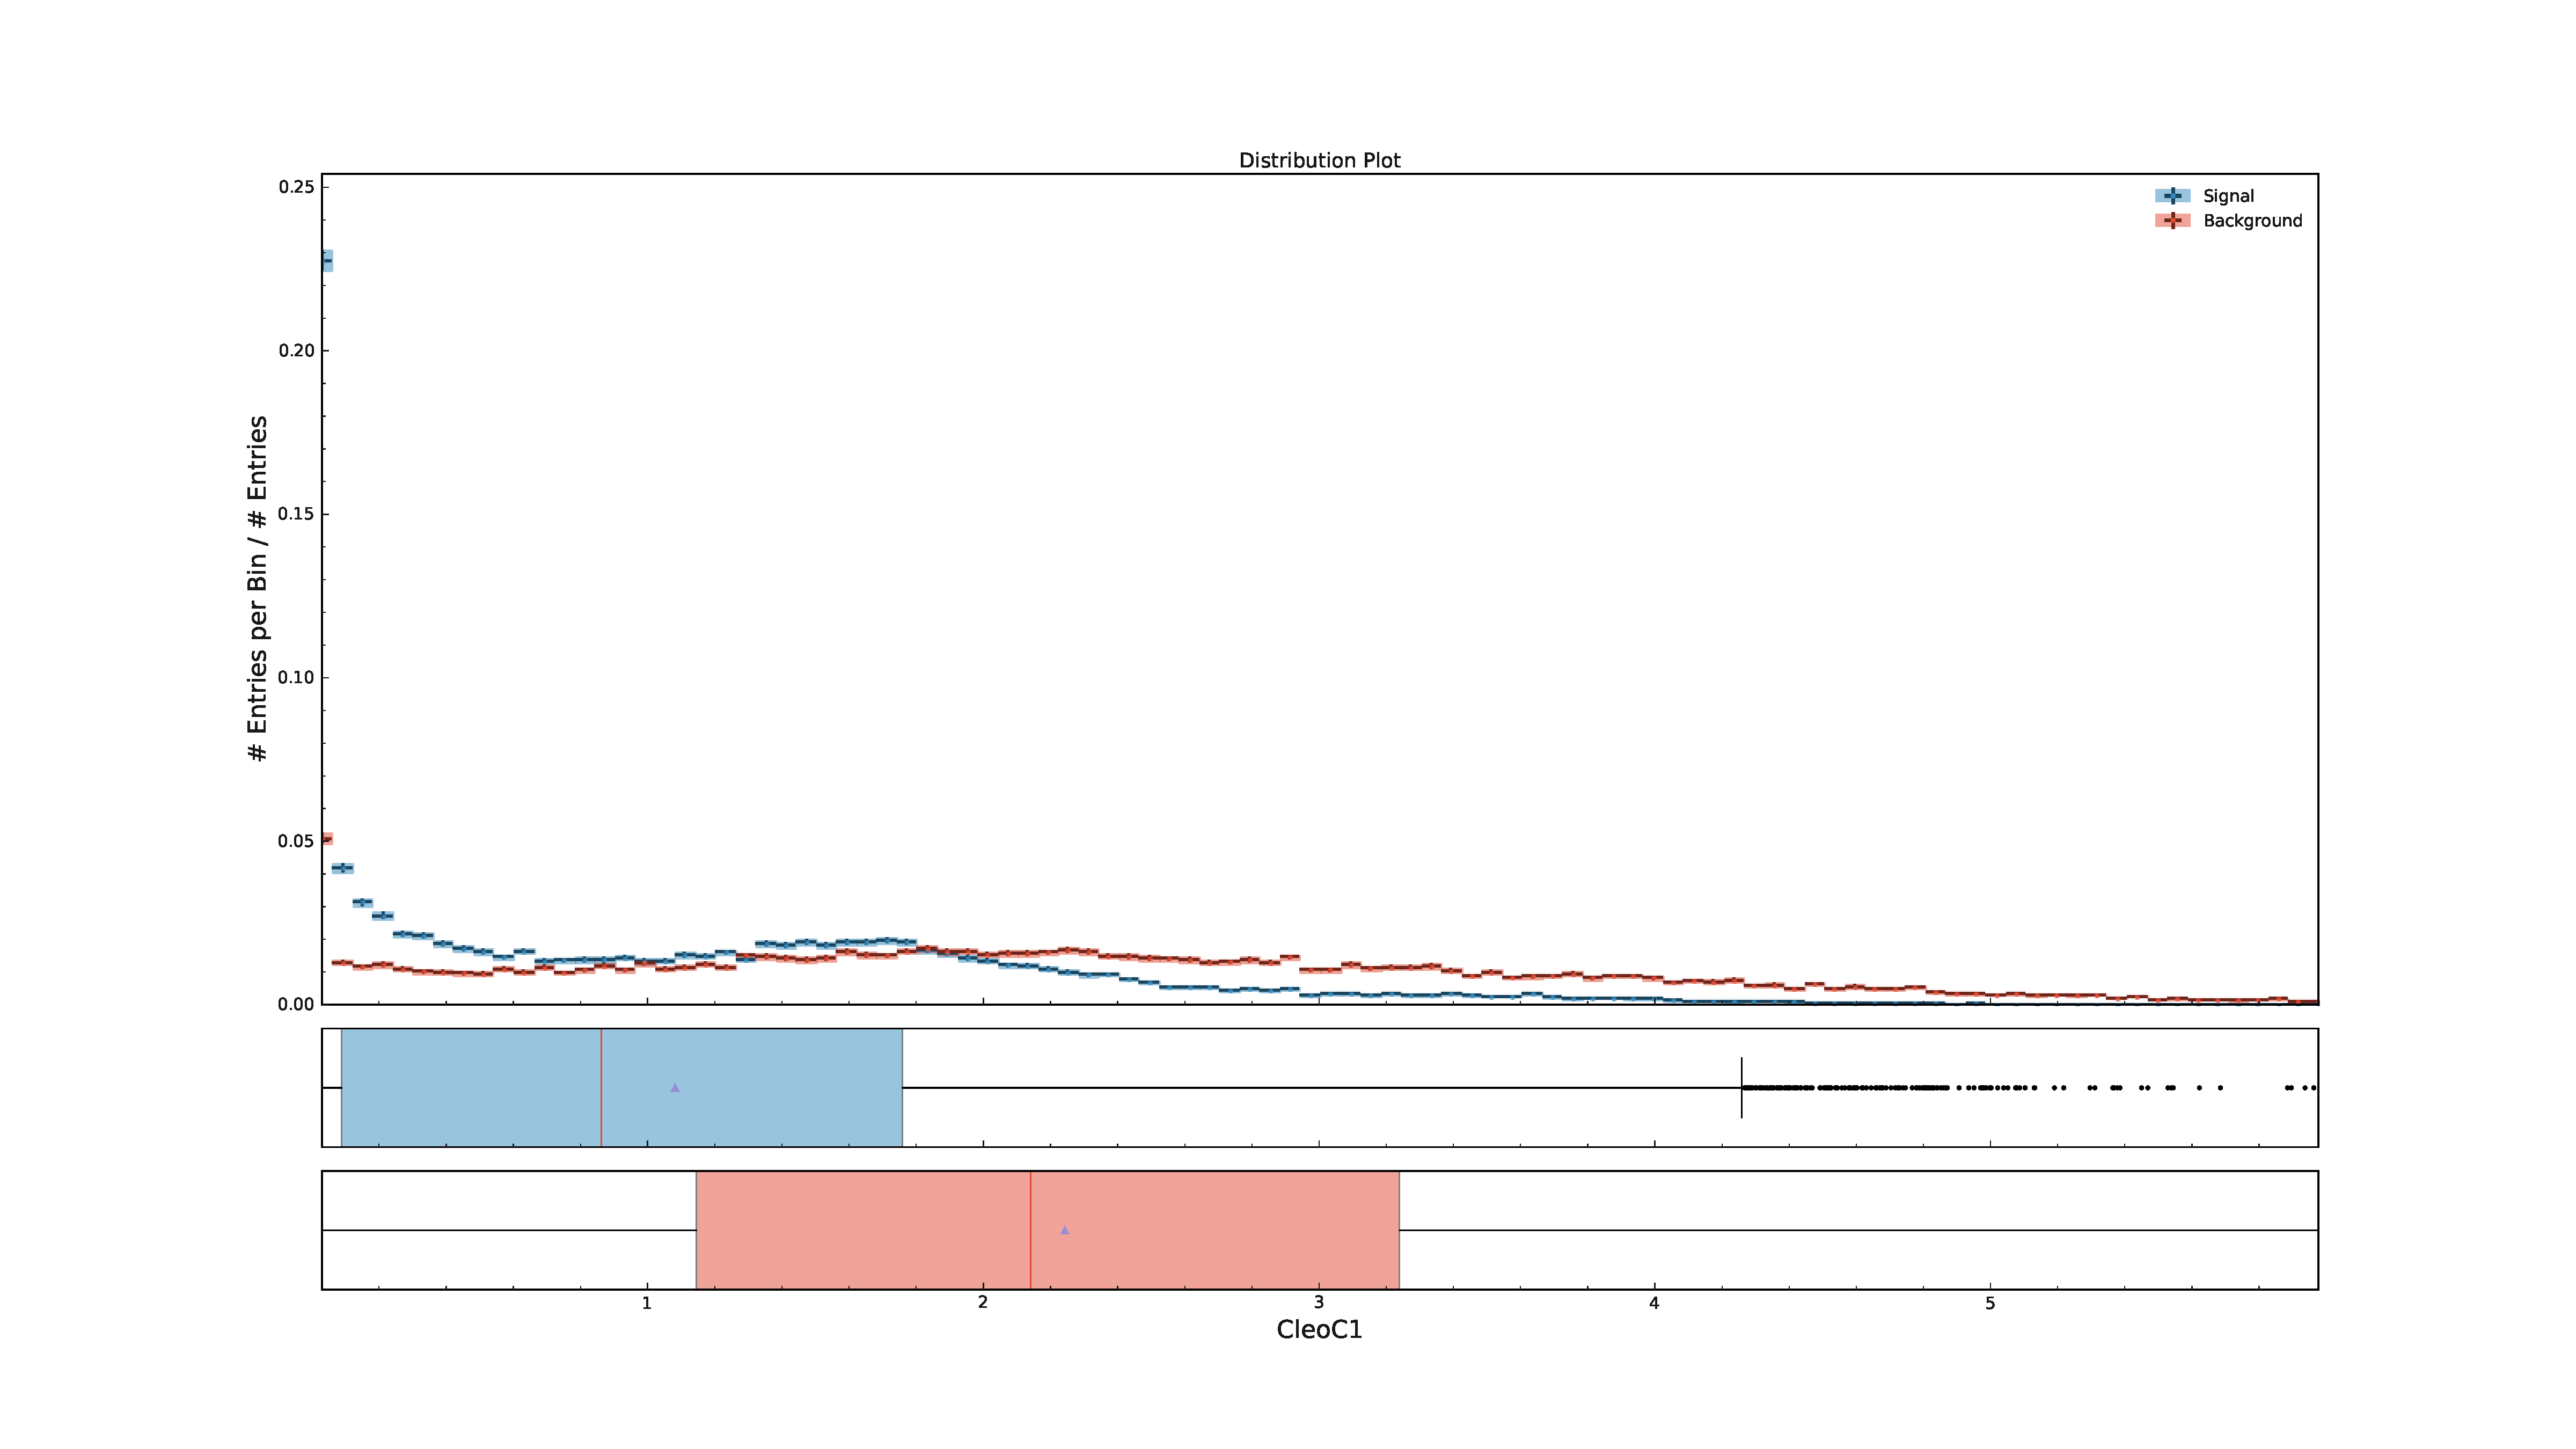
\includegraphics[width=1.0\textwidth]{variable_5452775316428386635.pdf}
\end{center}
\subsection{KSFWVariables(hoo0)}
\begin{center}
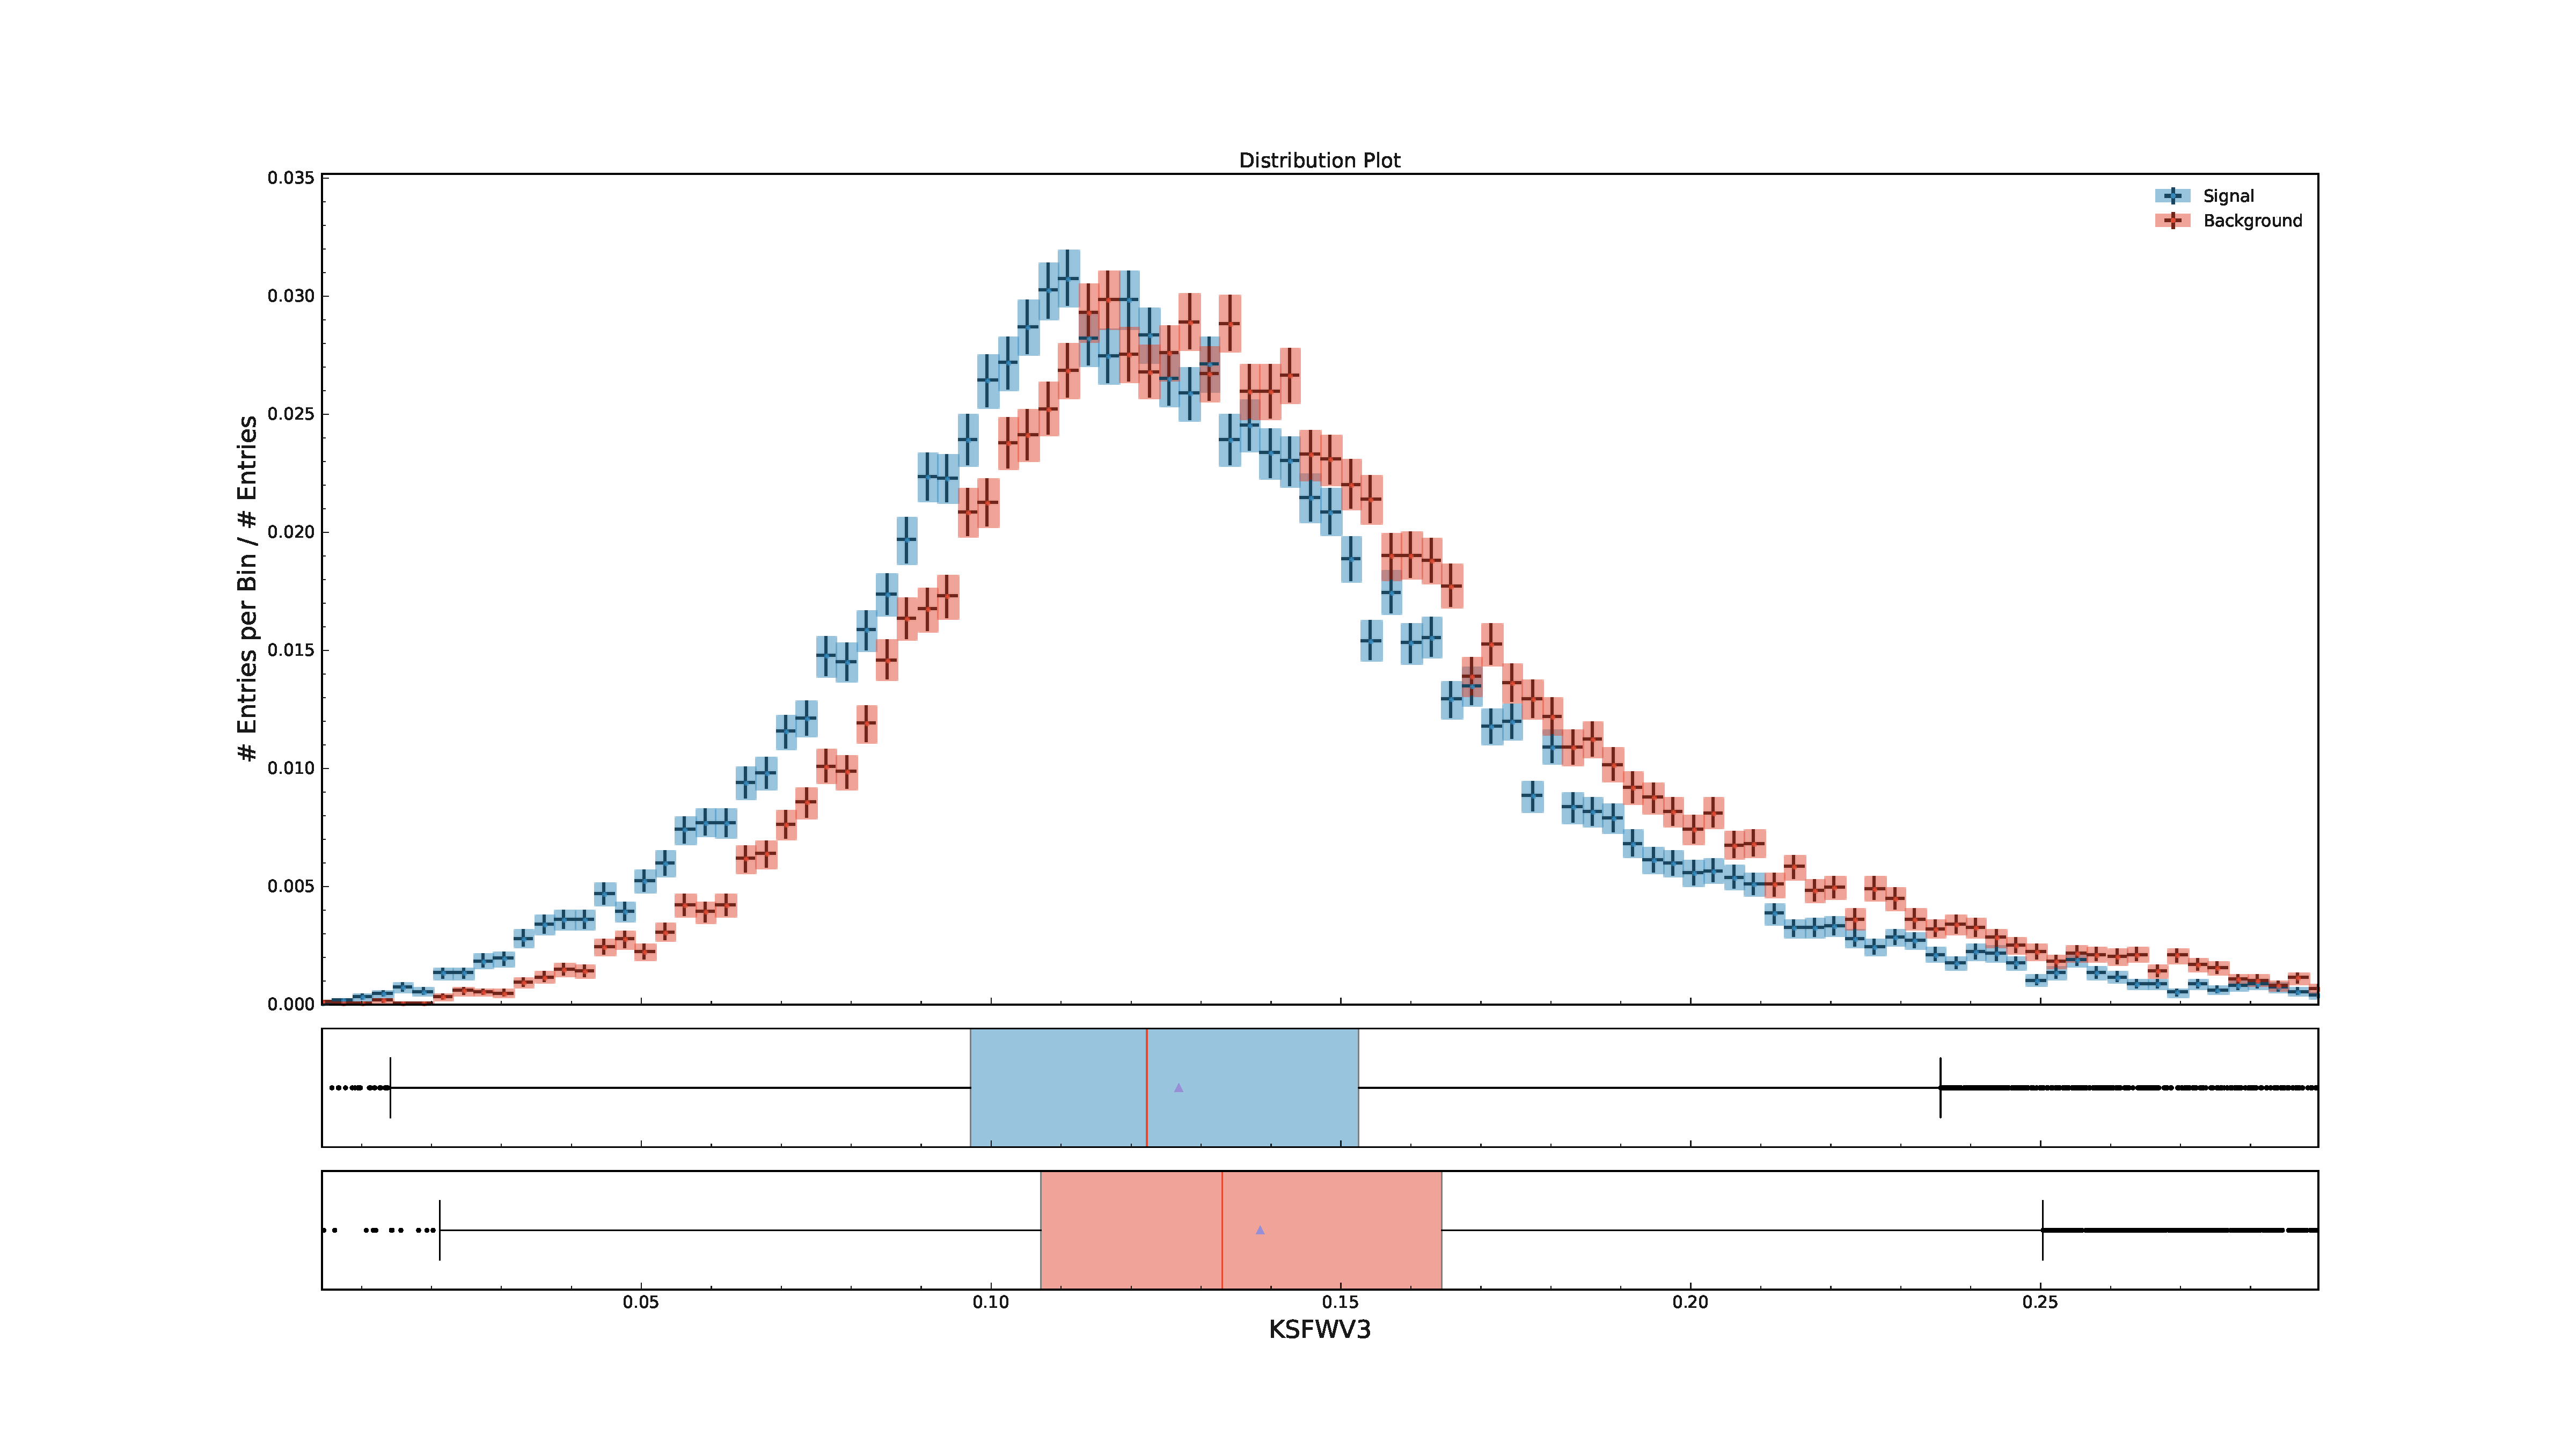
\includegraphics[width=1.0\textwidth]{variable_4125238112556289389.pdf}
\end{center}
\subsection{thrustOm}
\begin{center}
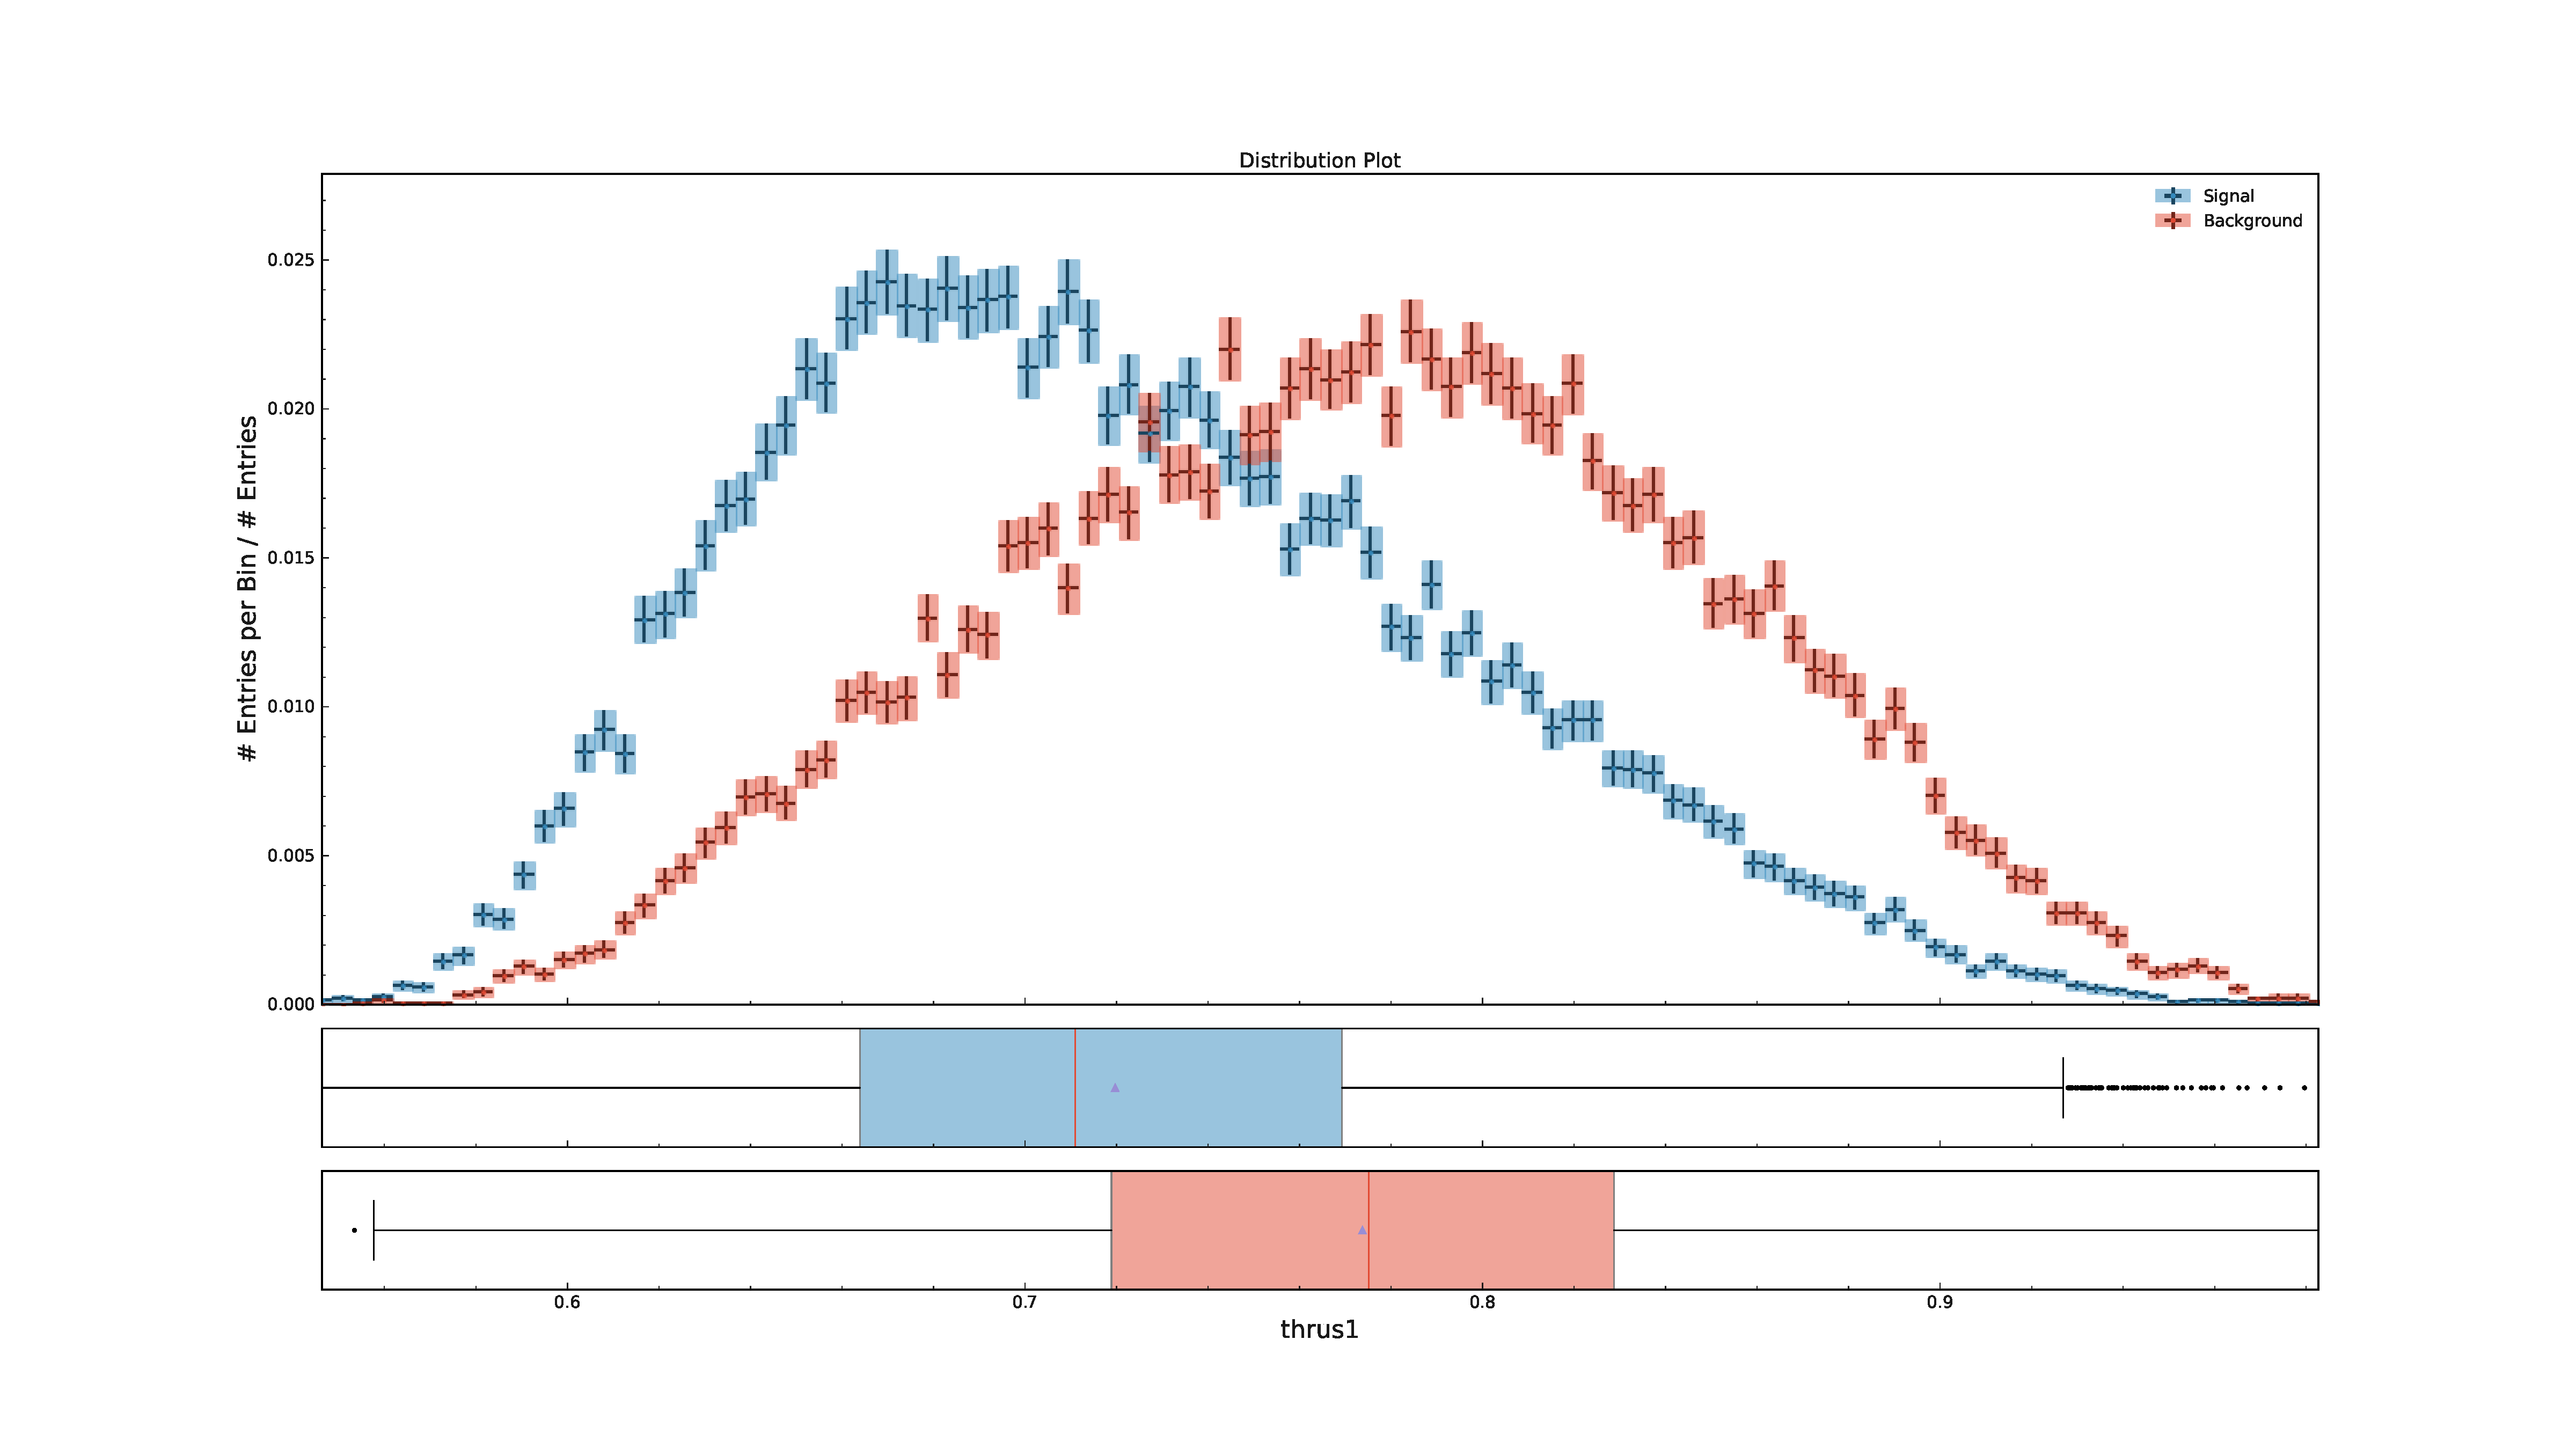
\includegraphics[width=1.0\textwidth]{variable_-1774228743304352852.pdf}
\end{center}
\subsection{KSFWVariables(et)}
\begin{center}
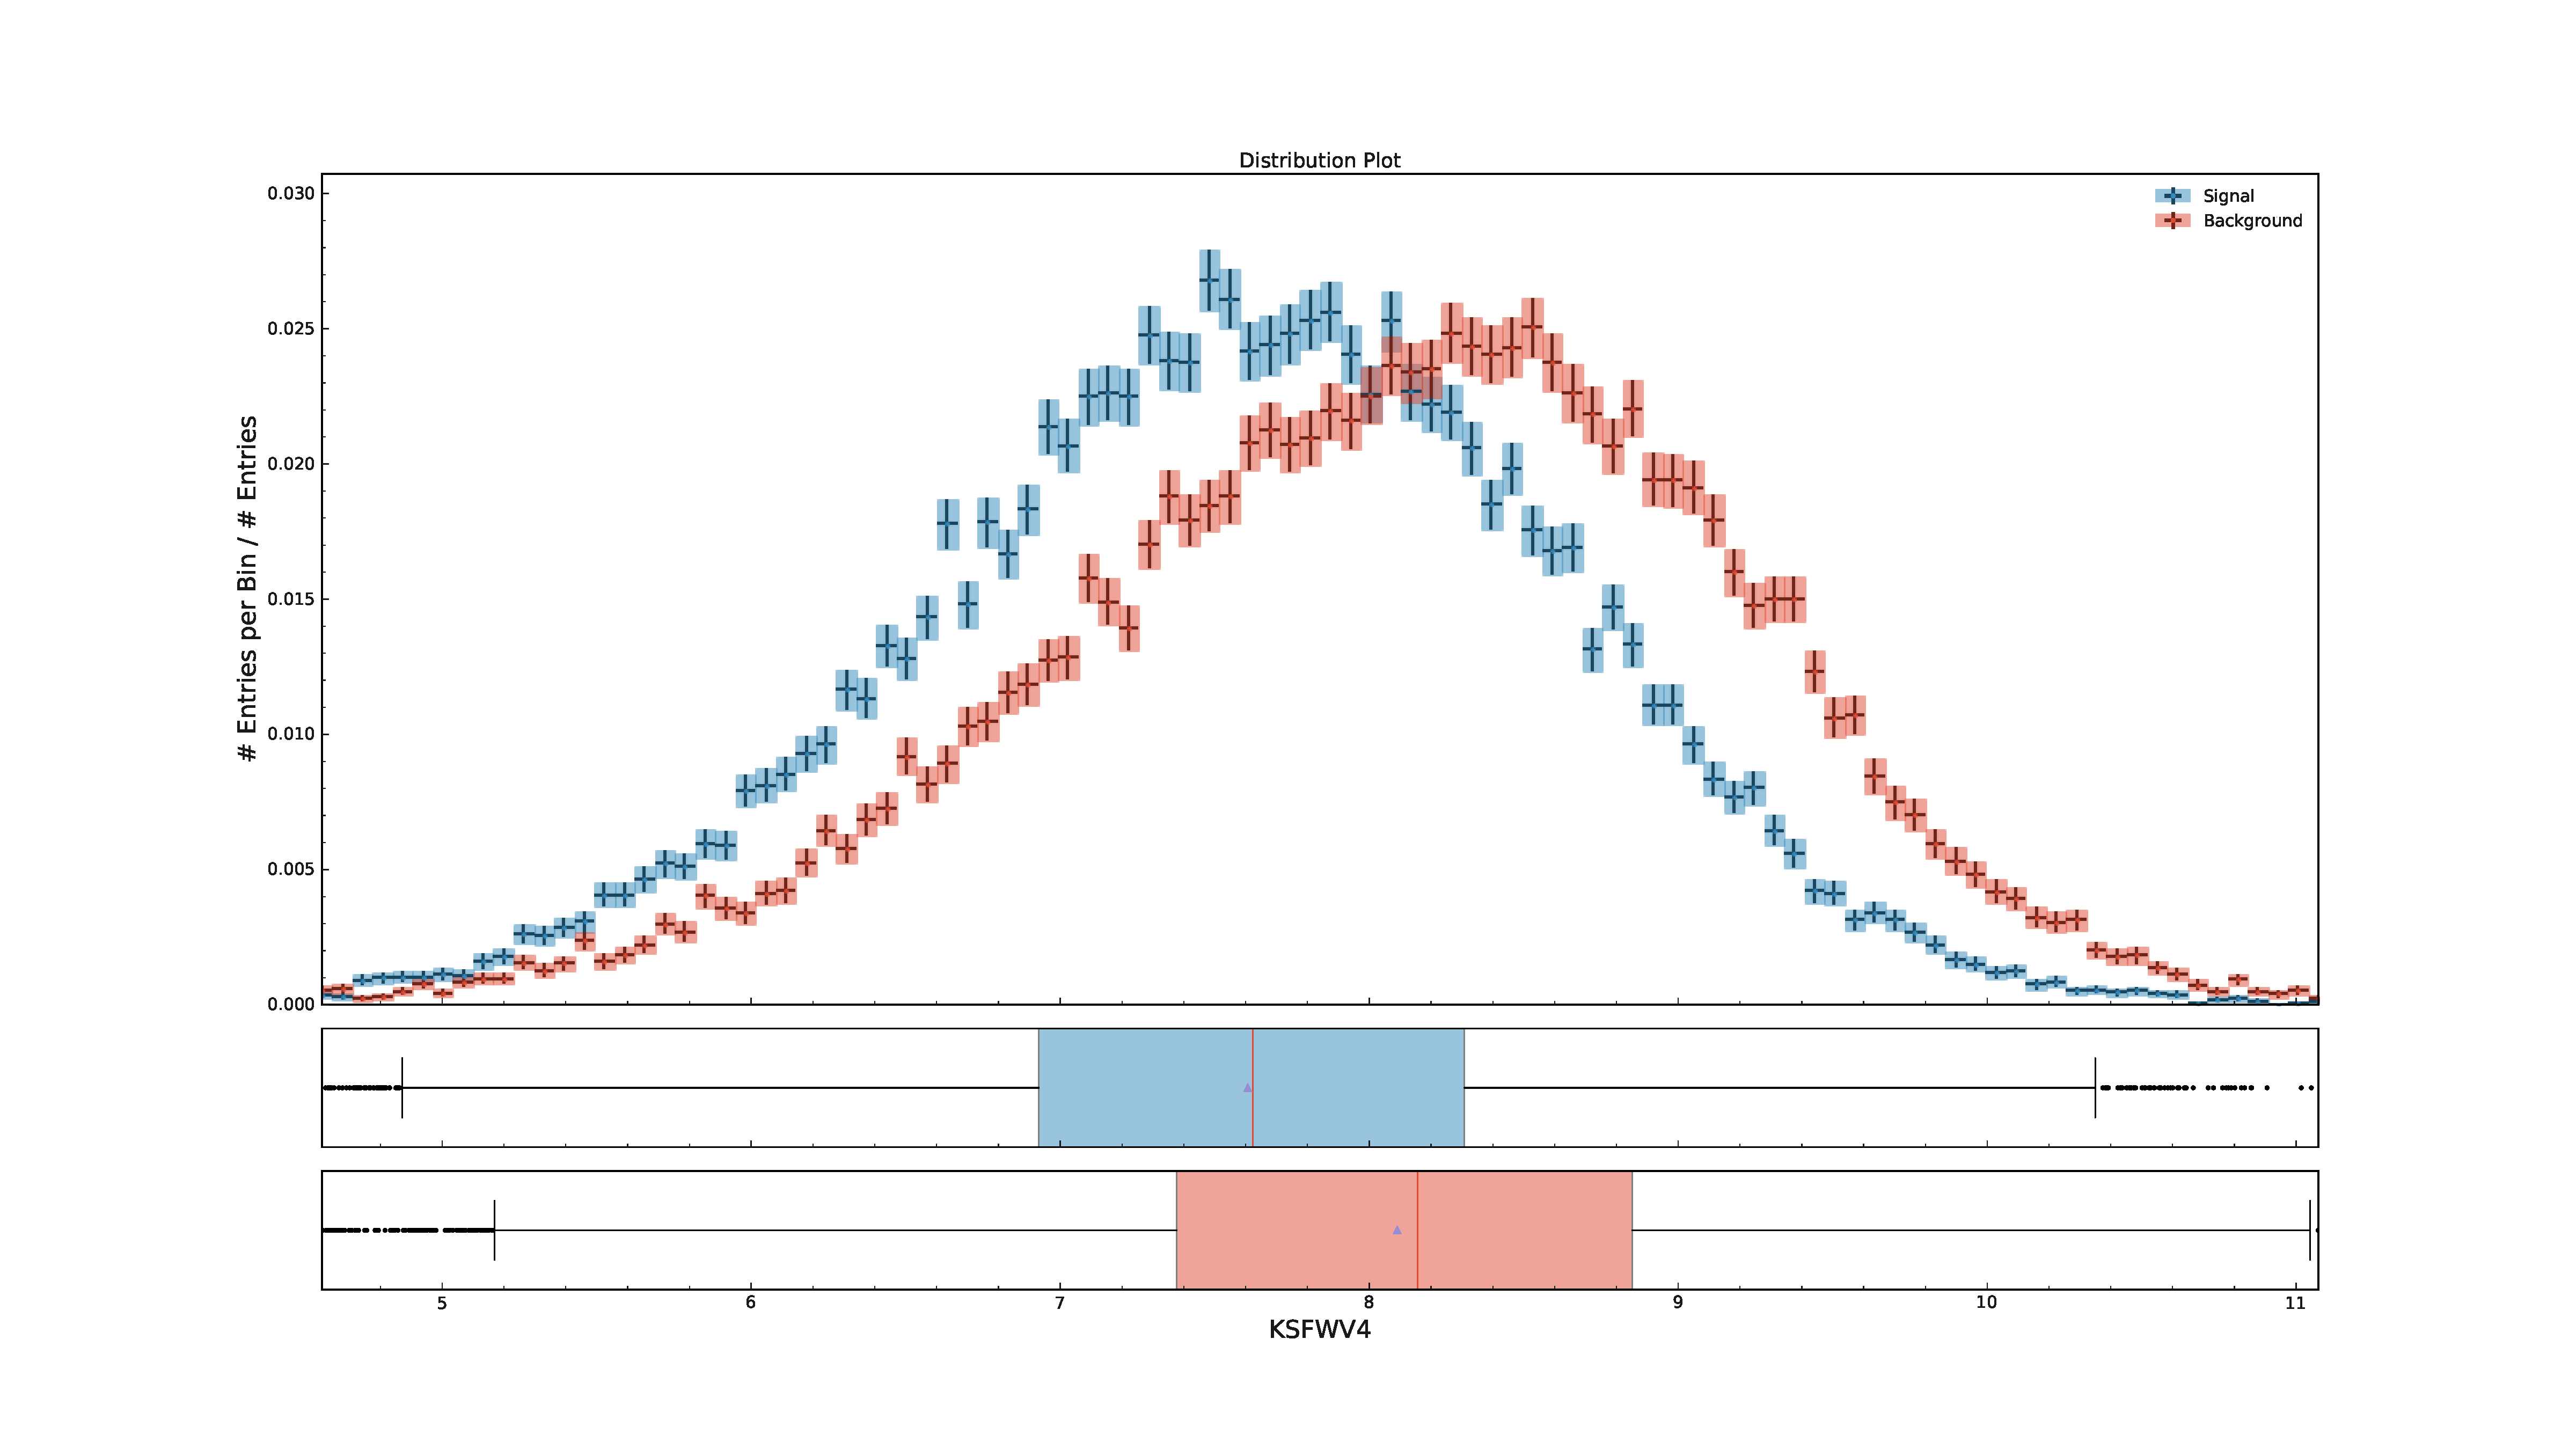
\includegraphics[width=1.0\textwidth]{variable_1627611668298853210.pdf}
\end{center}
\subsection{CleoConeCS(1)}
\begin{center}
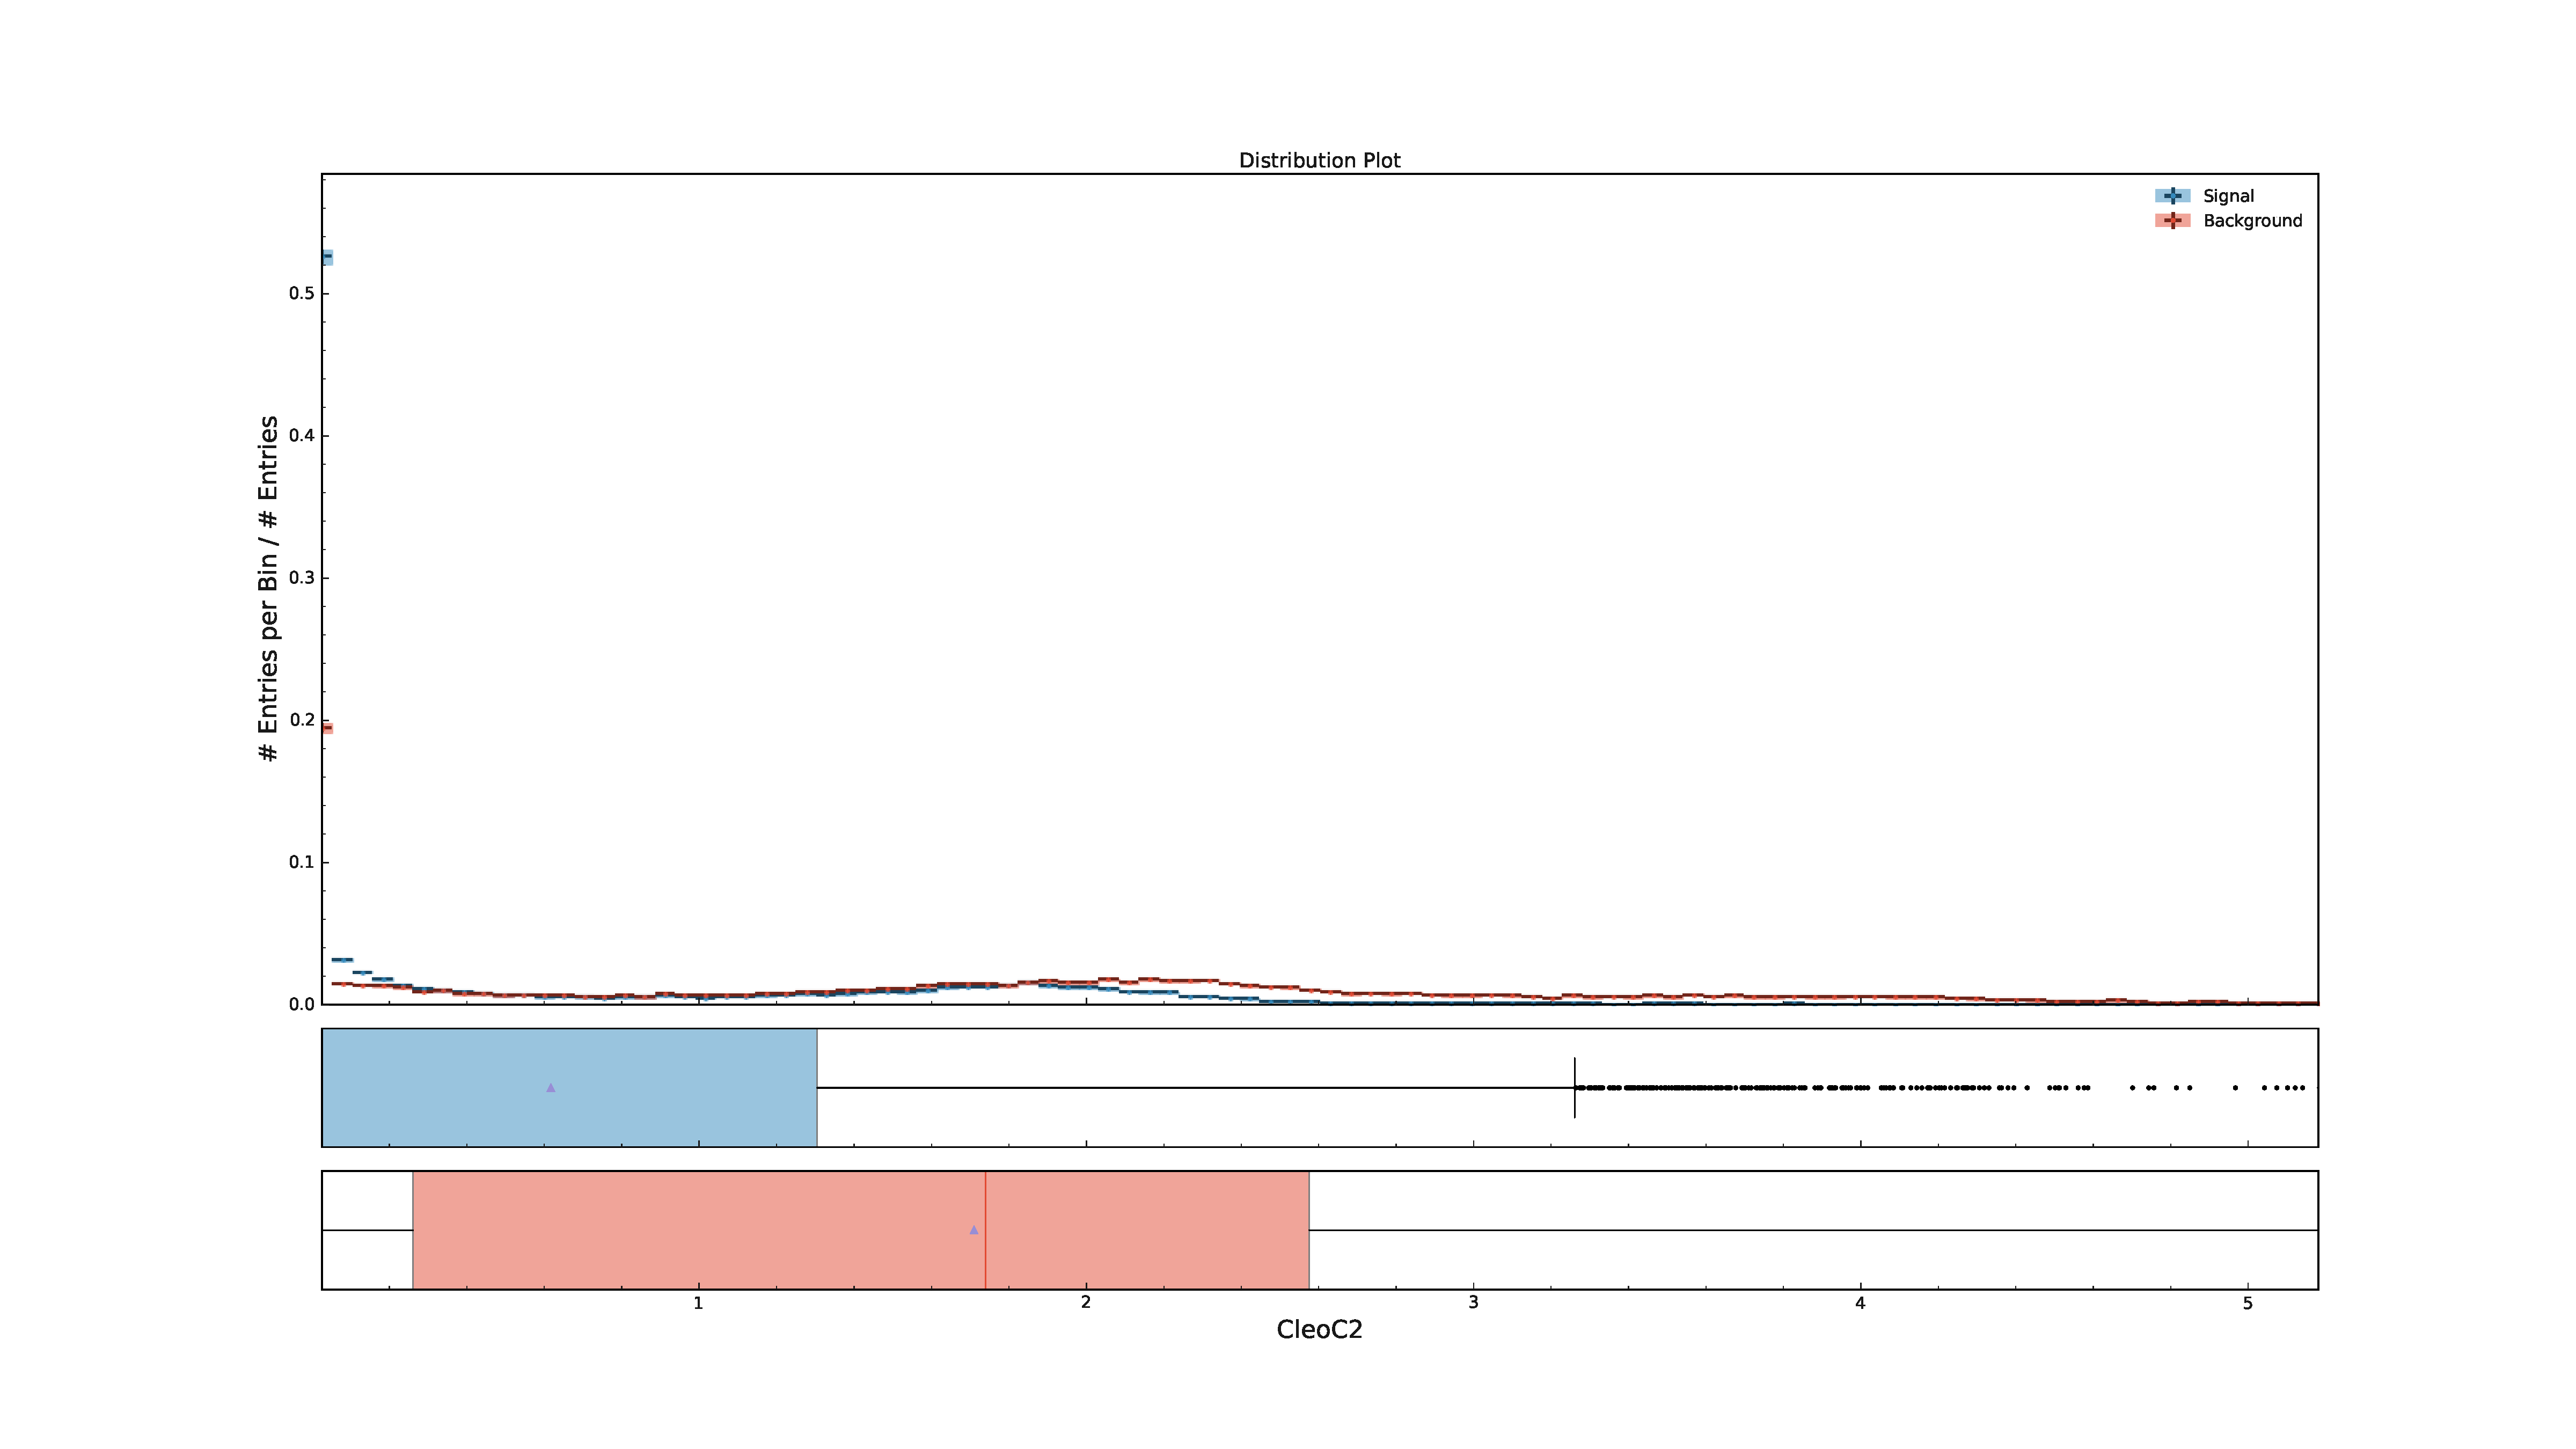
\includegraphics[width=1.0\textwidth]{variable_4296370140092378655.pdf}
\end{center}
\subsection{cosTBz}
\begin{center}
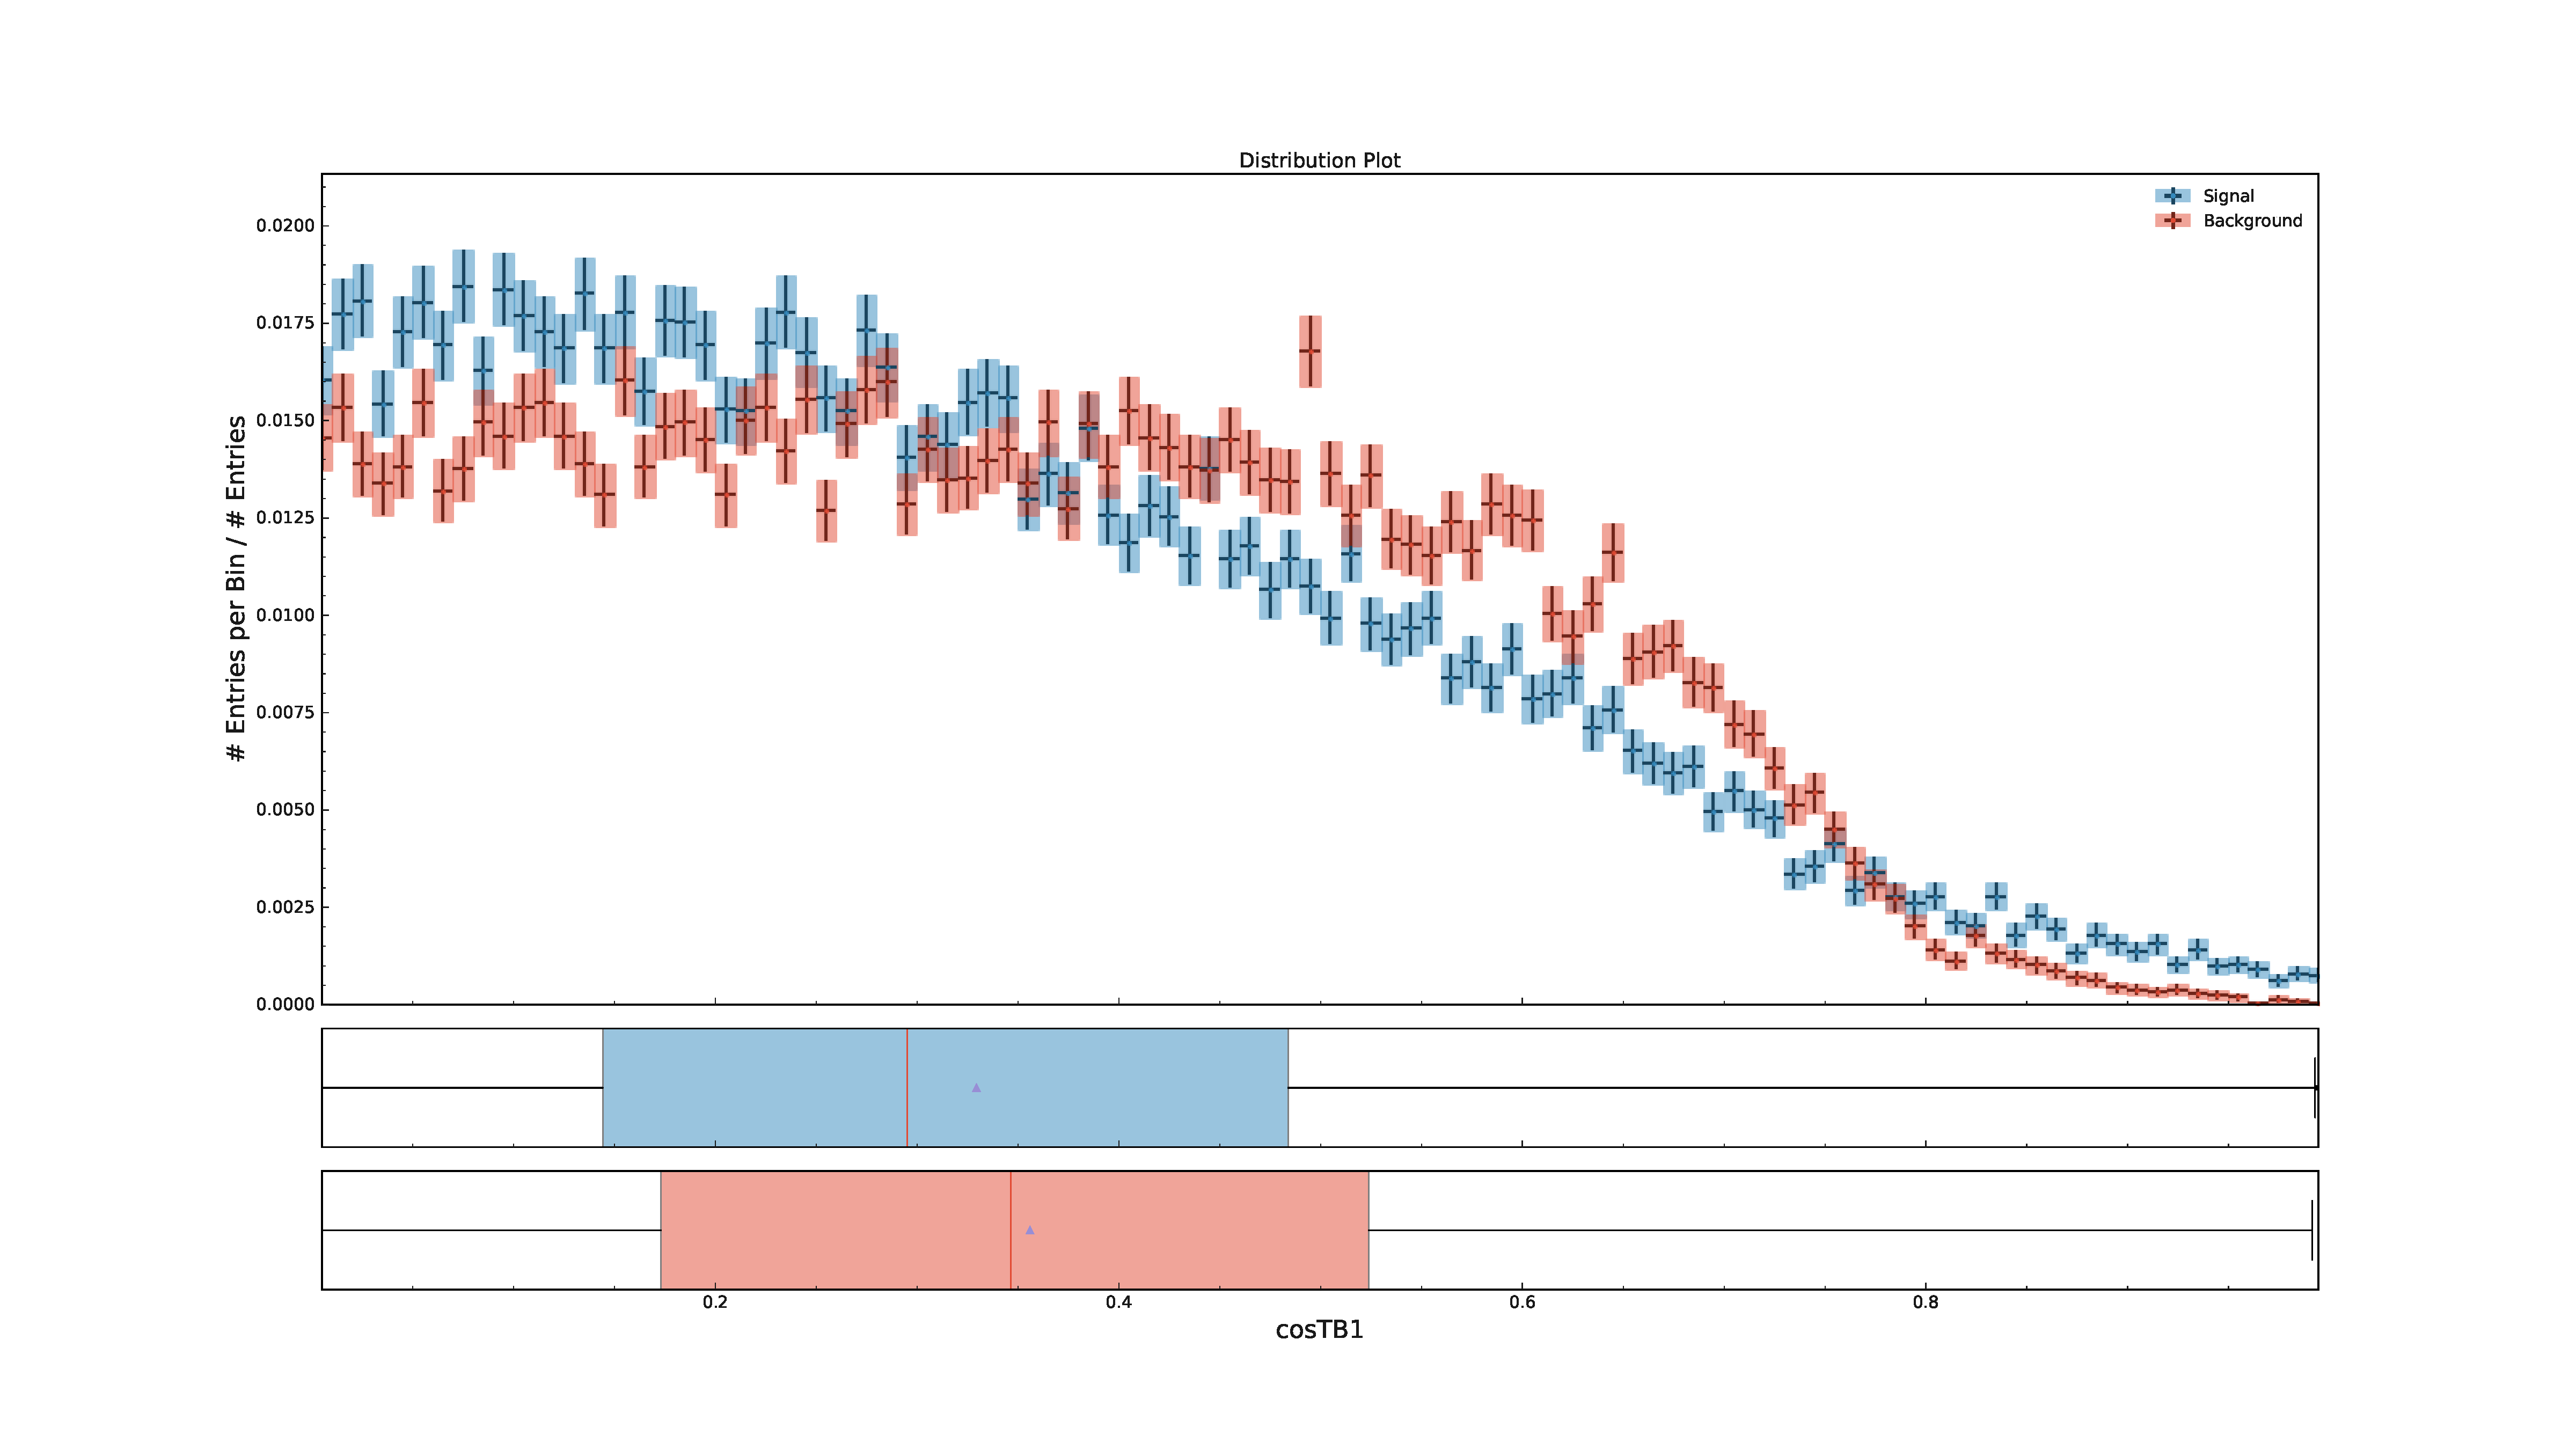
\includegraphics[width=1.0\textwidth]{variable_6524522569690219926.pdf}
\end{center}
\subsection{KSFWVariables(hso10)}
\begin{center}
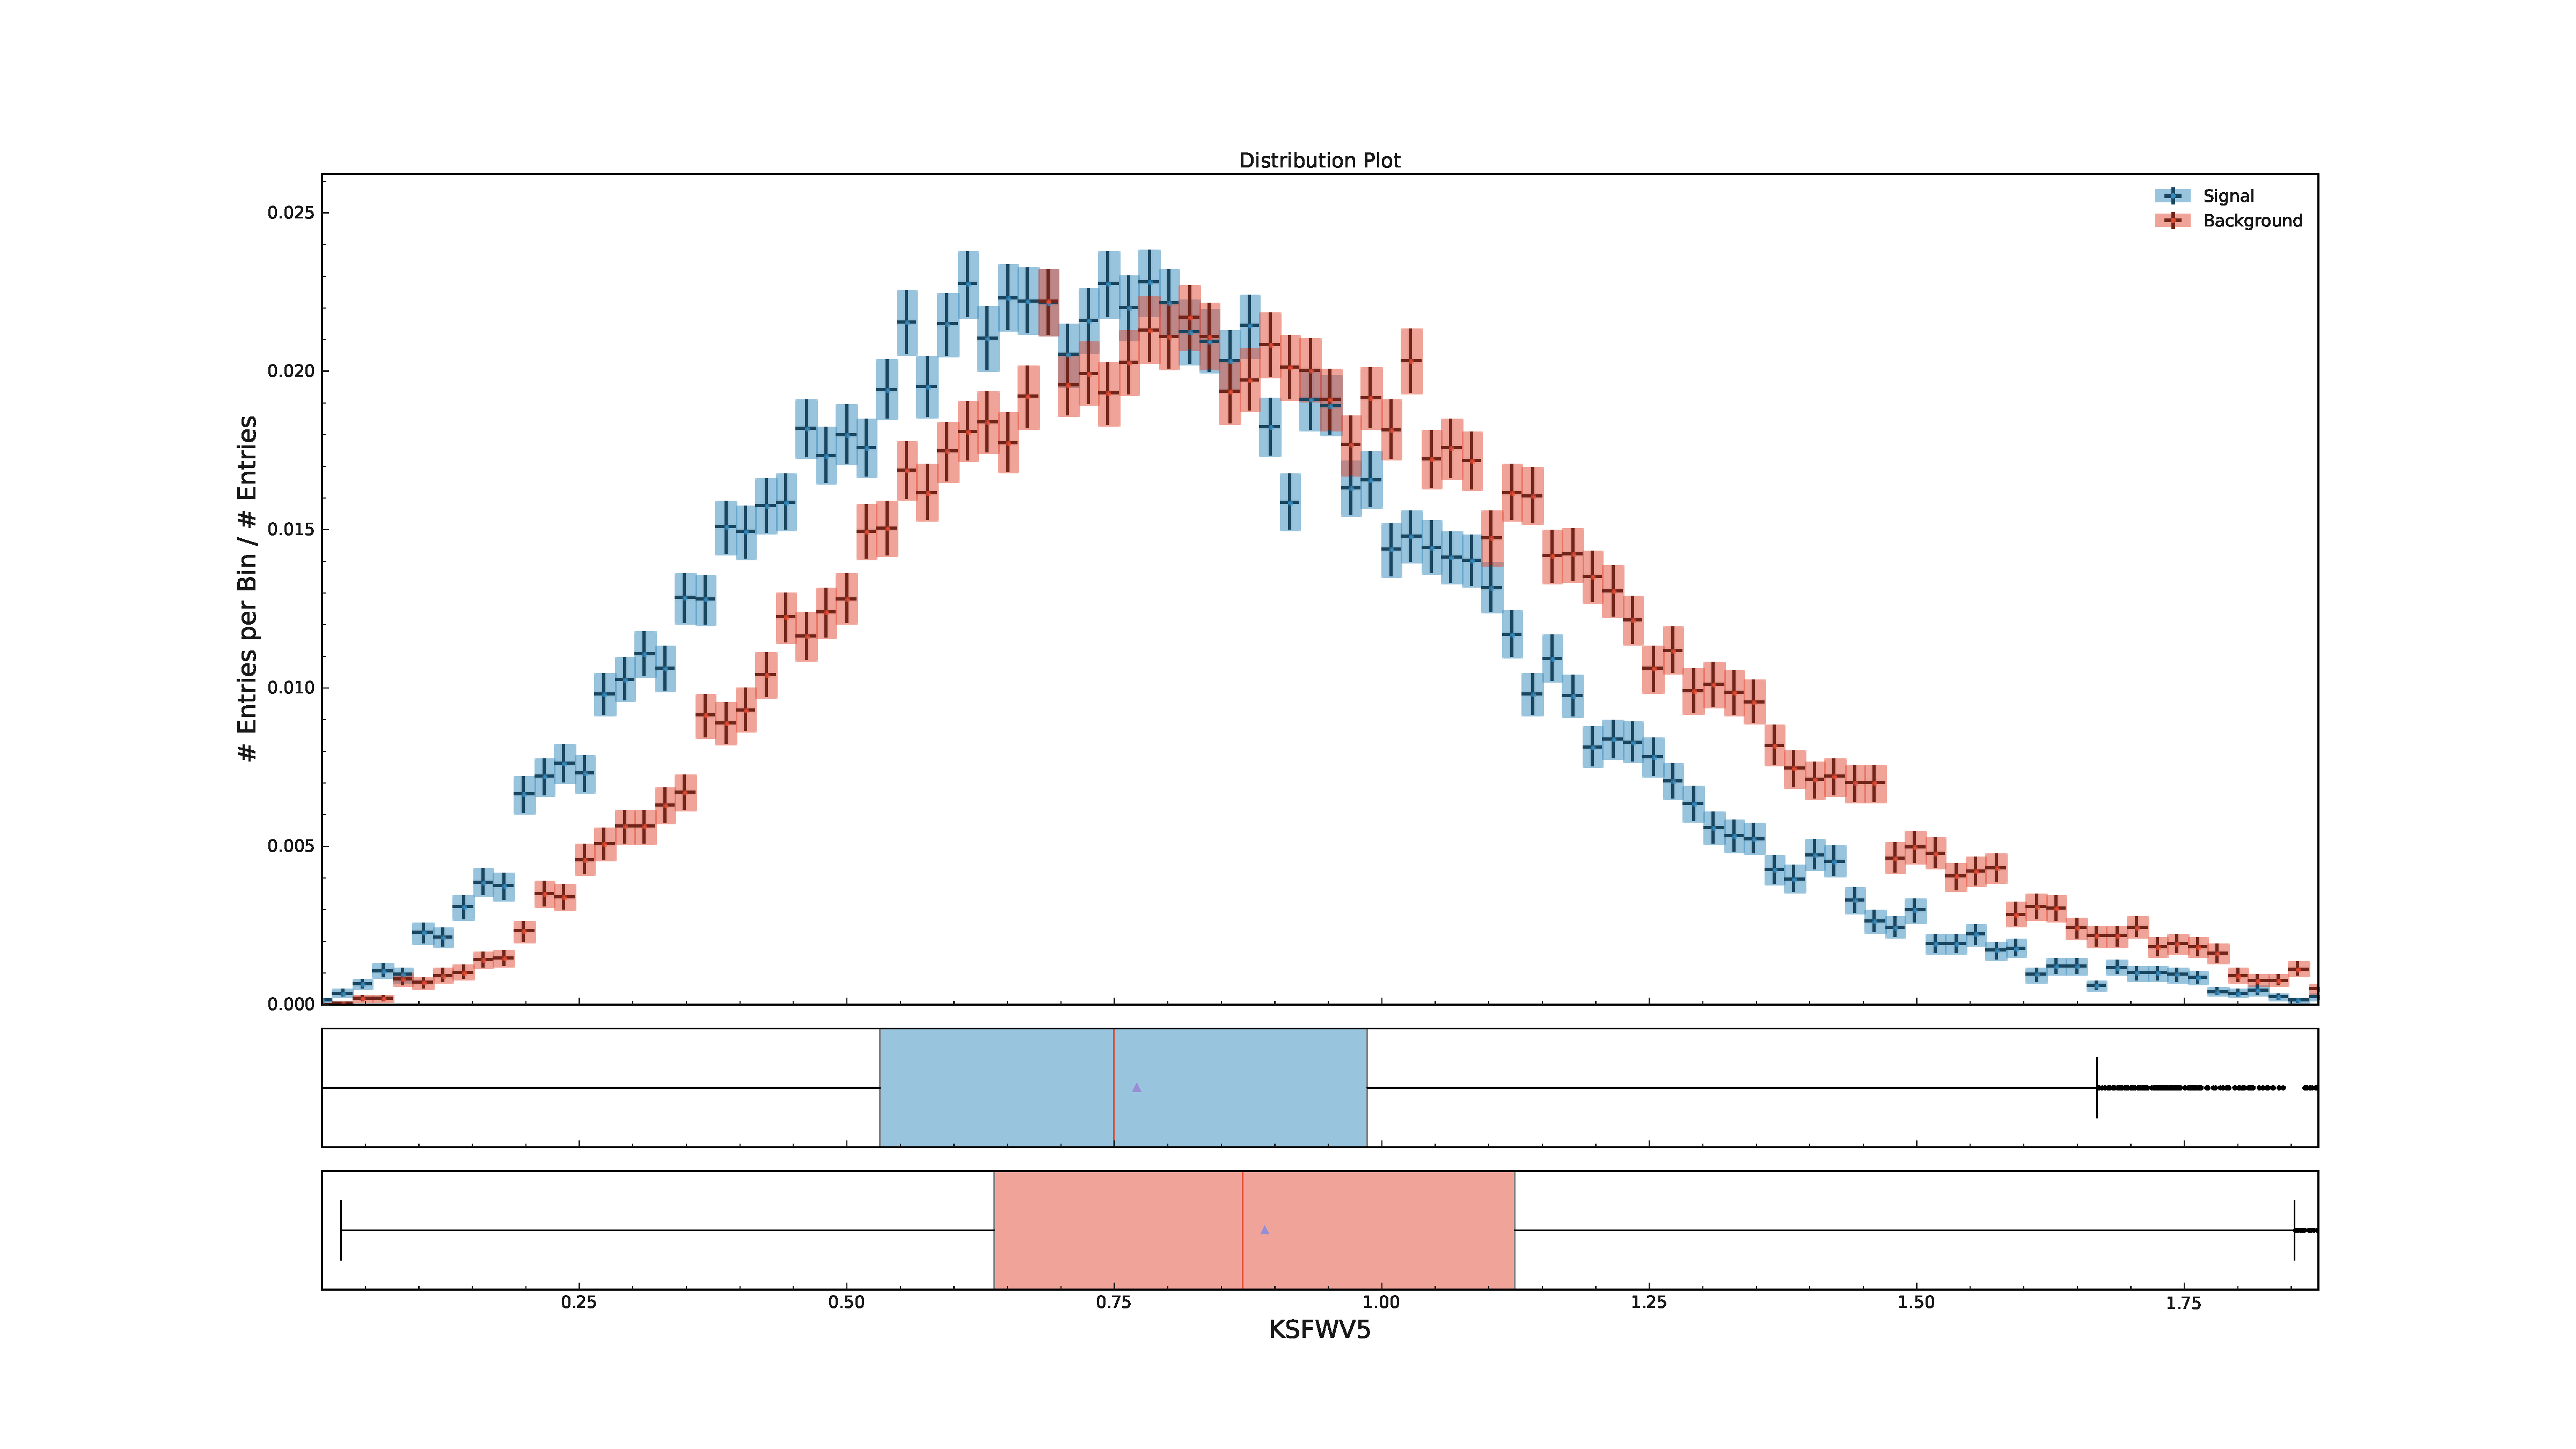
\includegraphics[width=1.0\textwidth]{variable_-8906981202890984423.pdf}
\end{center}
\subsection{KSFWVariables(hso02)}
\begin{center}
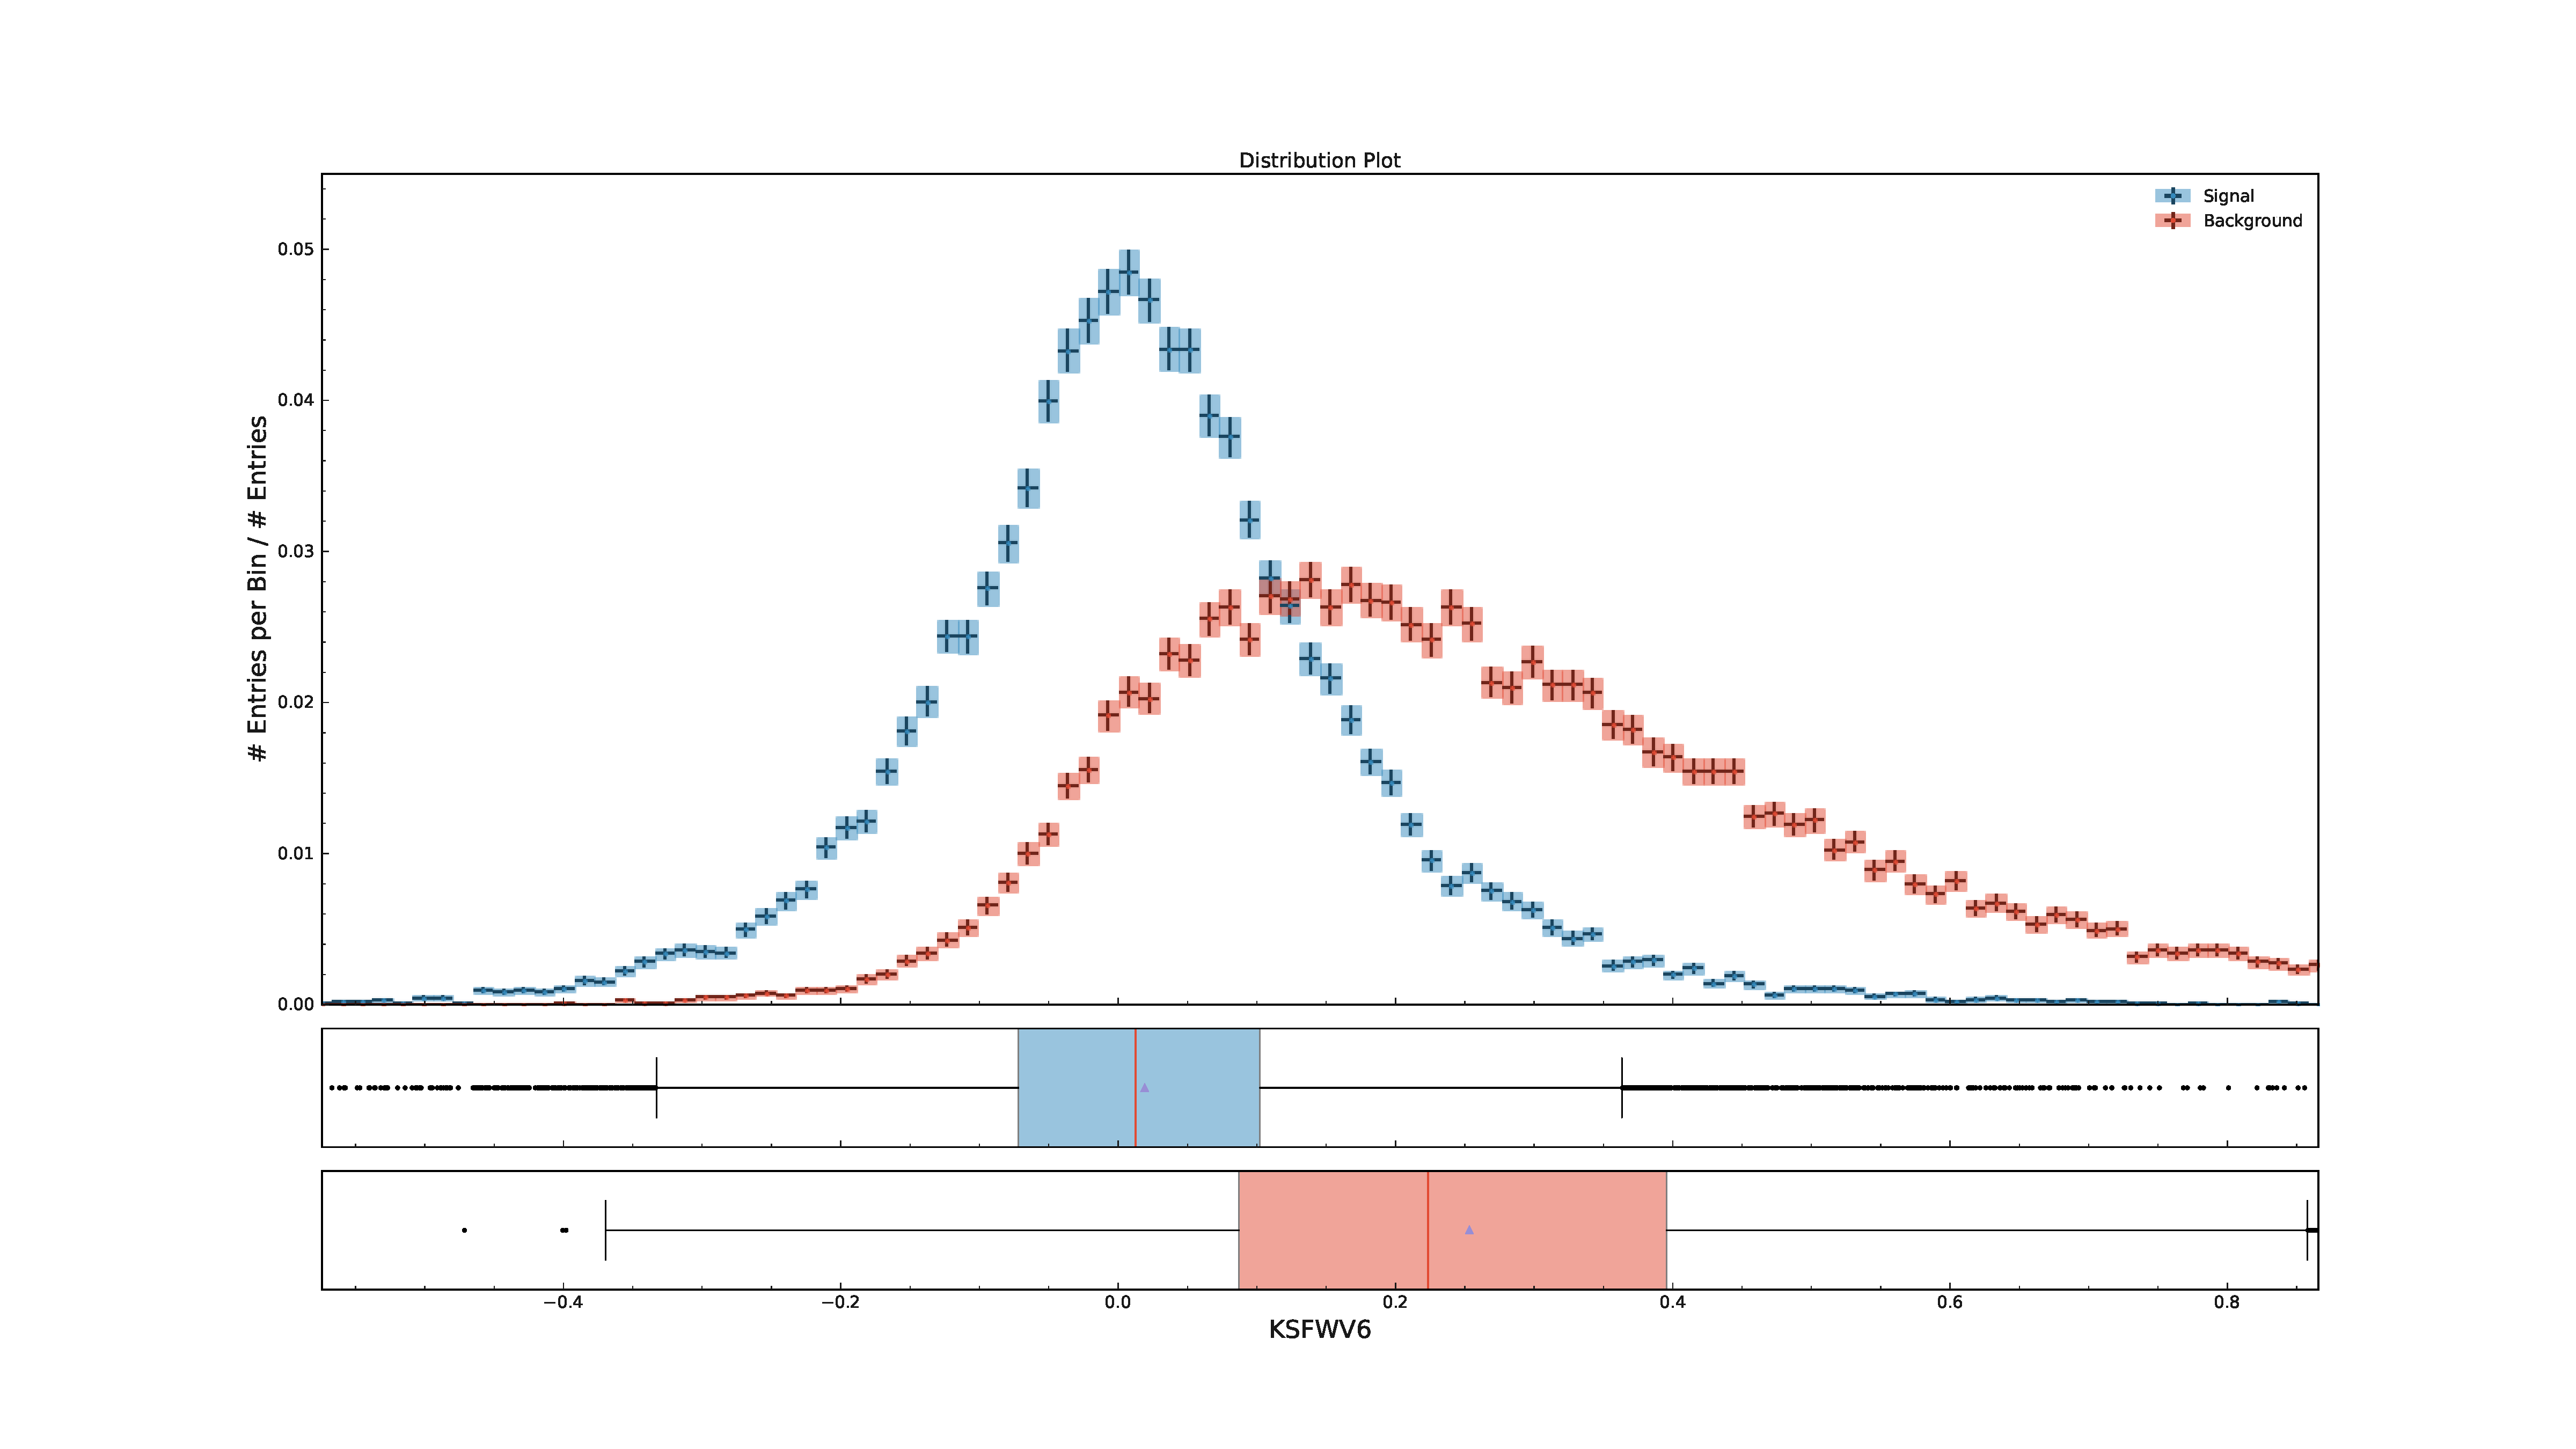
\includegraphics[width=1.0\textwidth]{variable_-5110443991643032712.pdf}
\end{center}
\subsection{KSFWVariables(hso12)}
\begin{center}
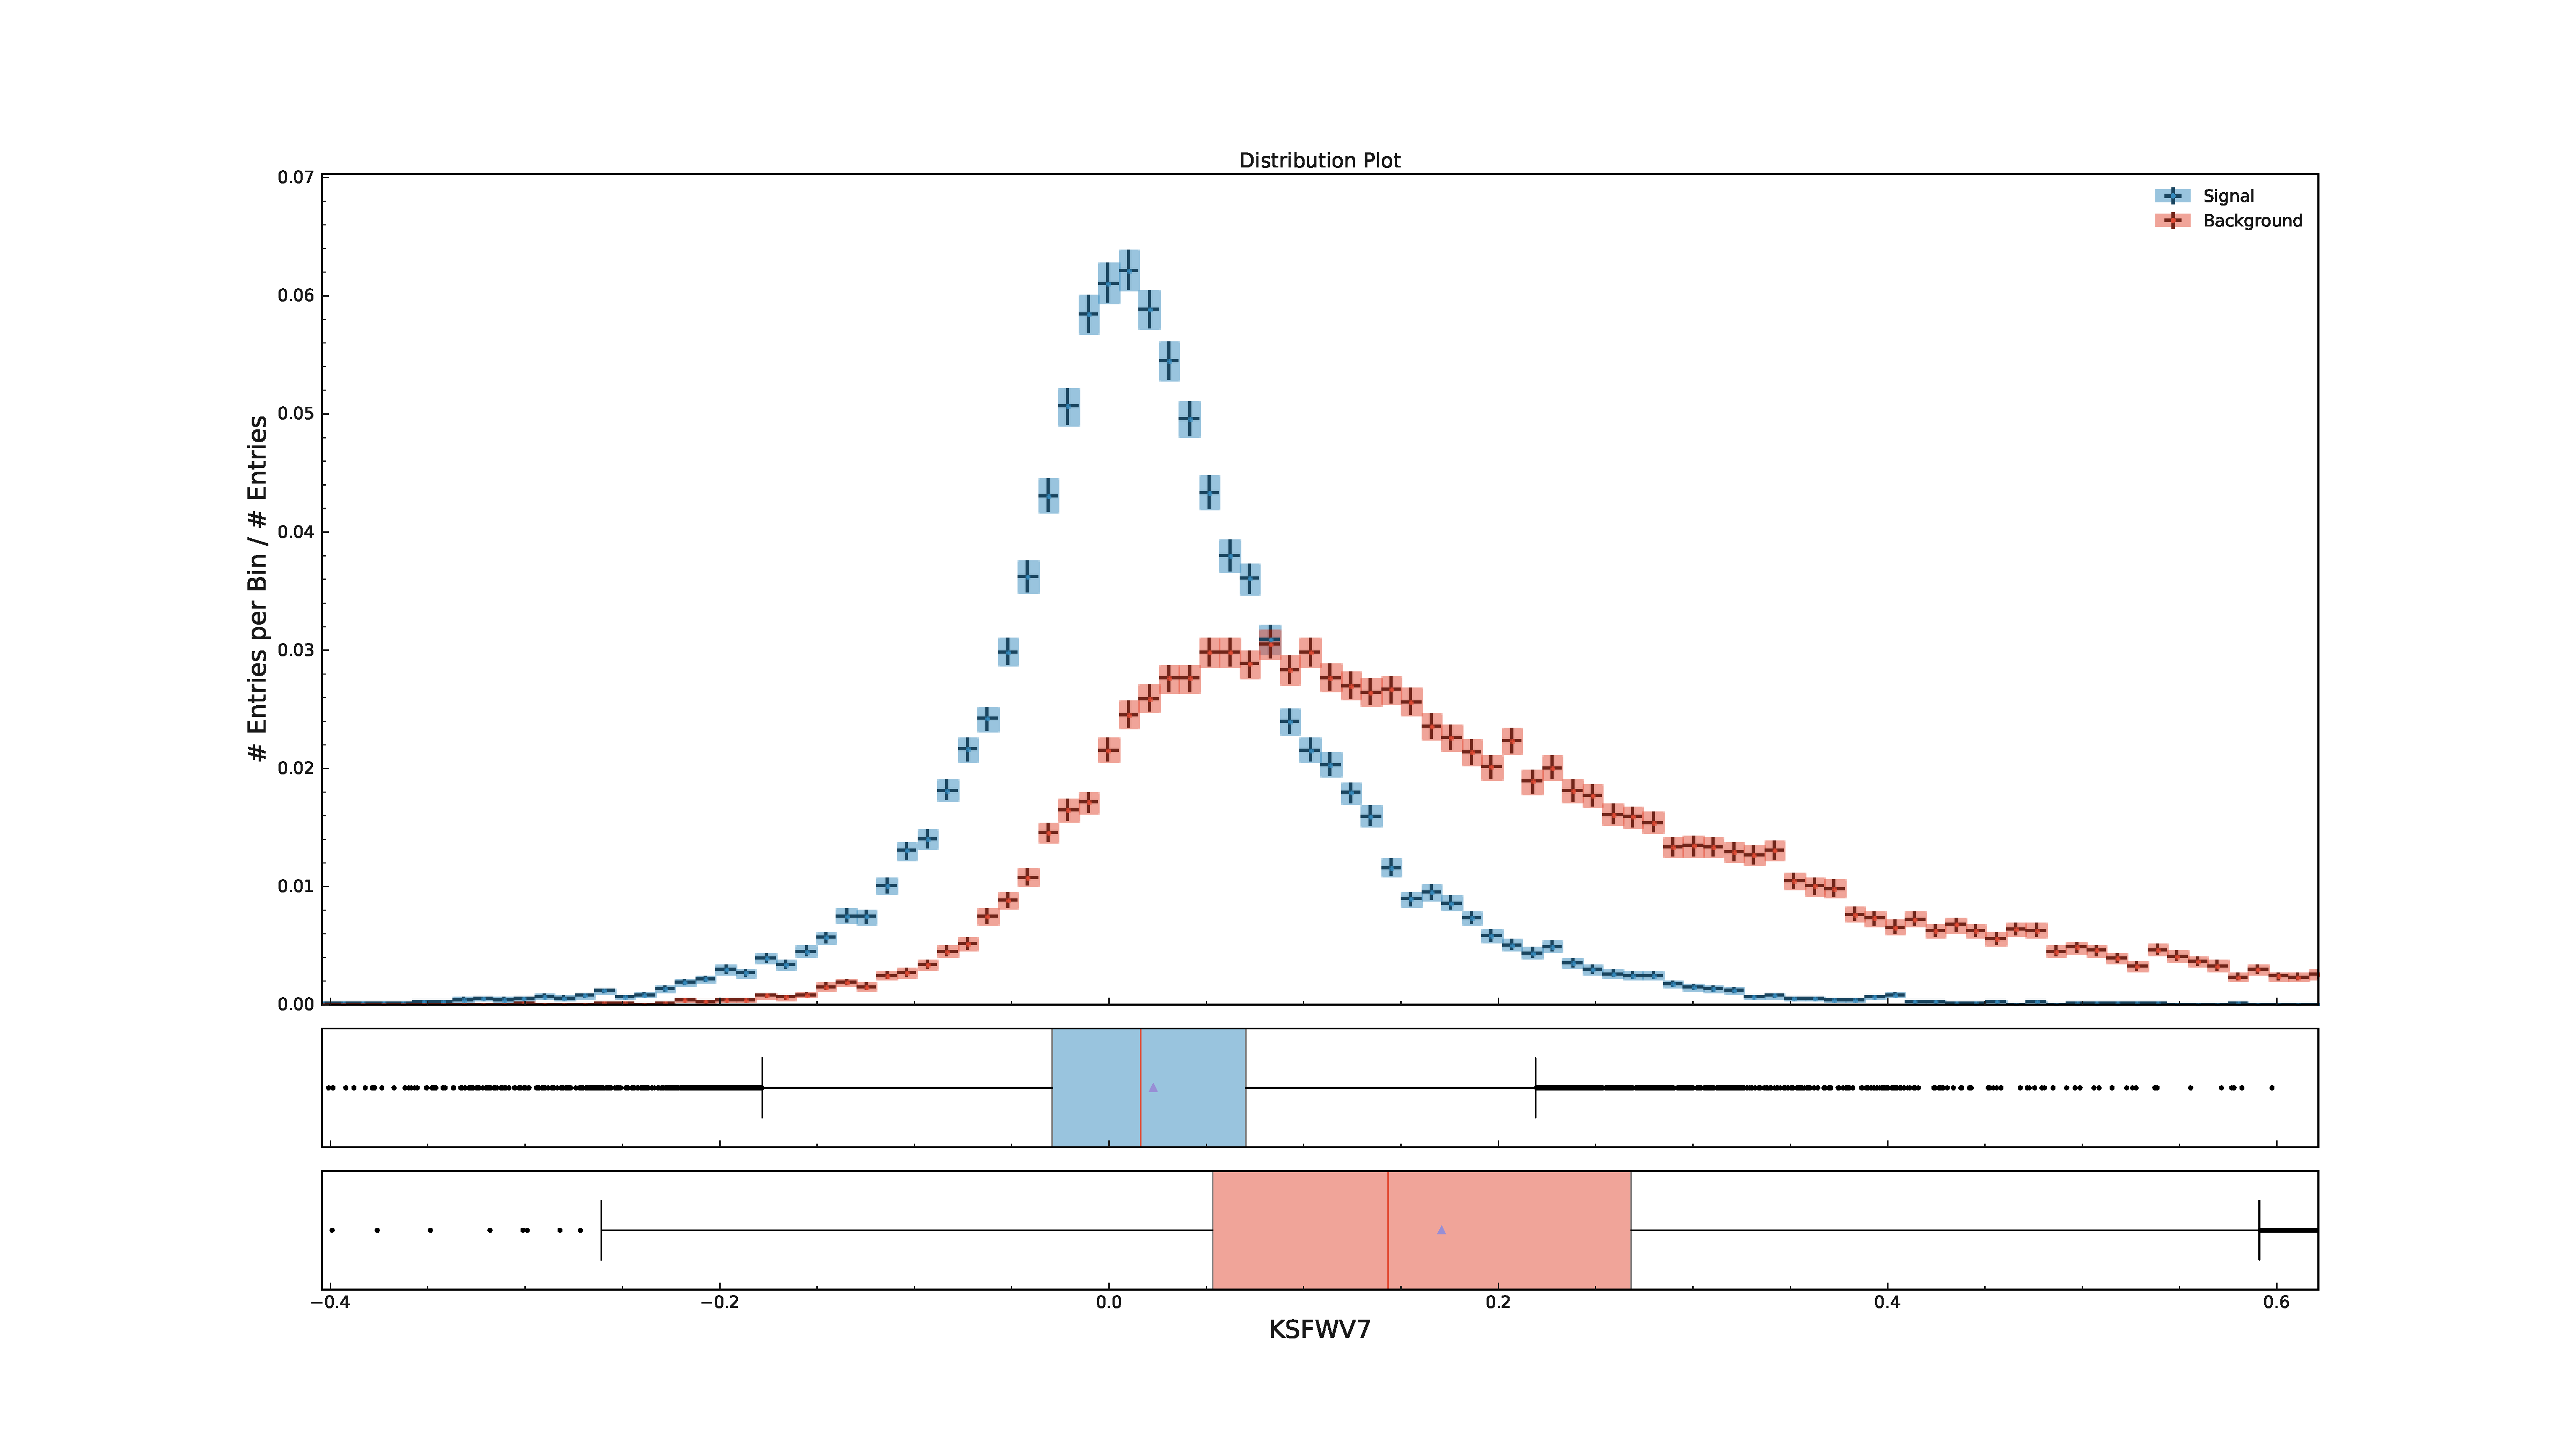
\includegraphics[width=1.0\textwidth]{variable_-5361807685078173071.pdf}
\end{center}
\subsection{CMS\_cosTheta}
\begin{center}
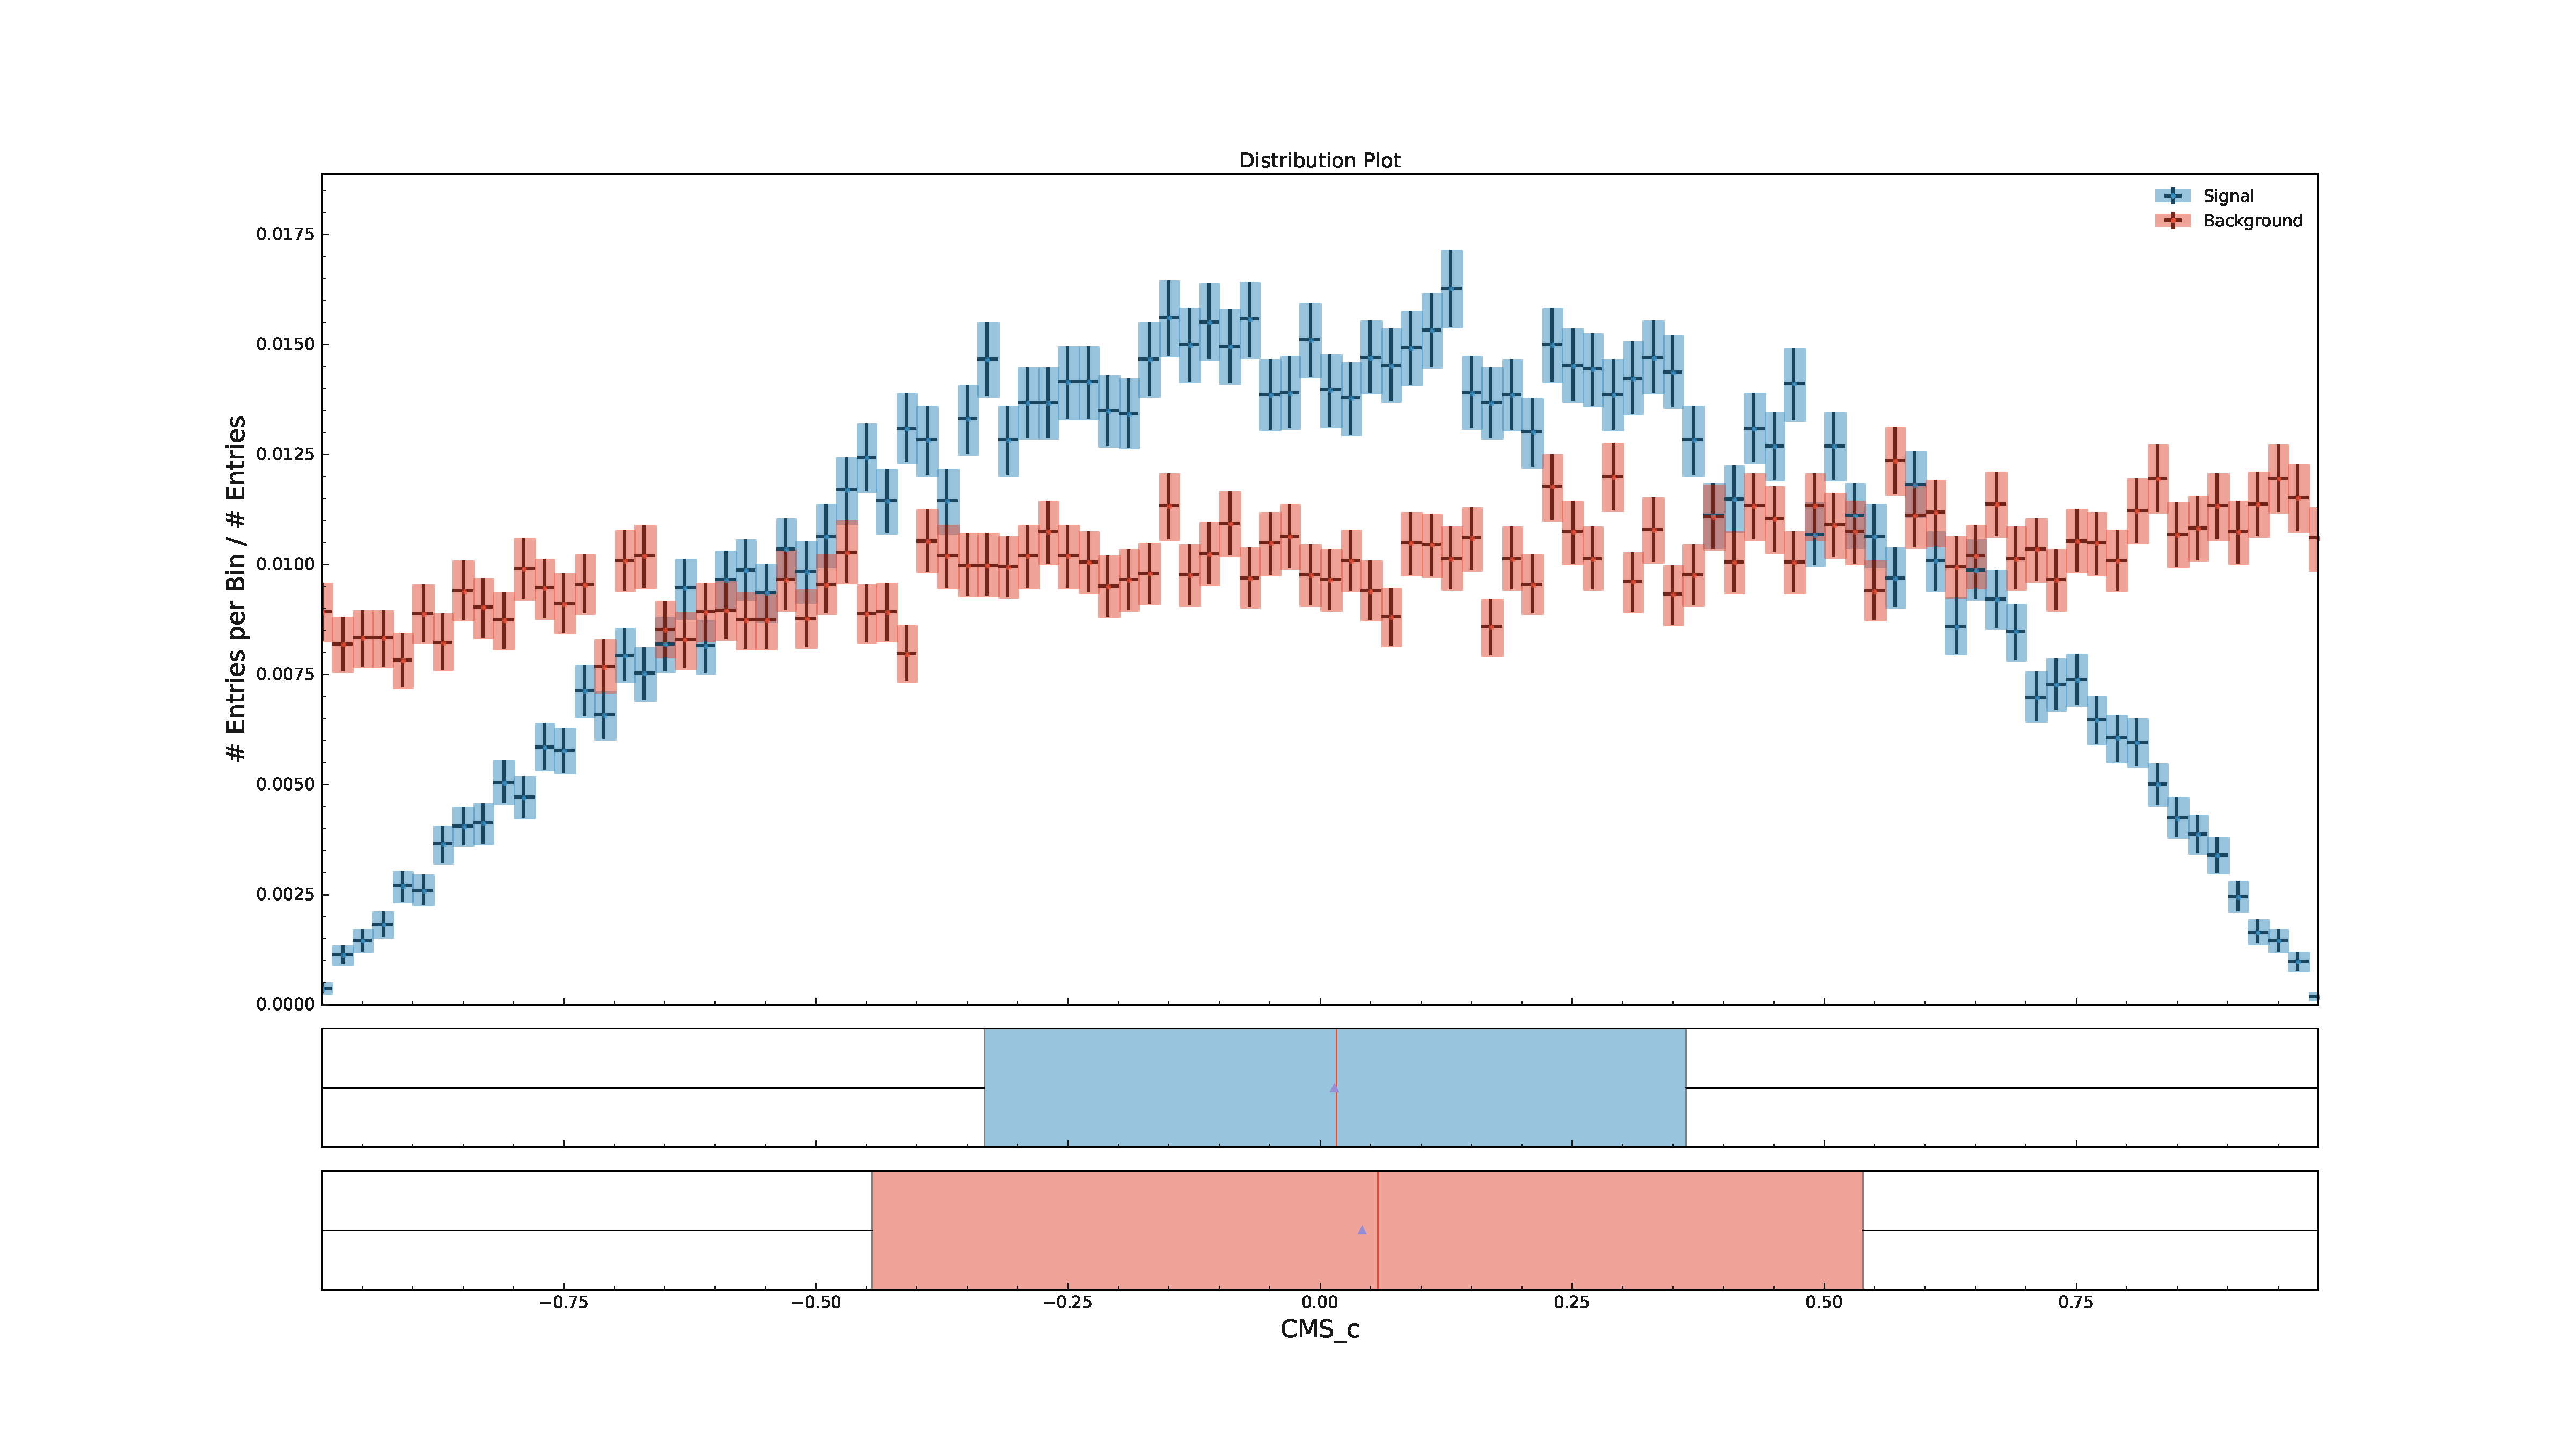
\includegraphics[width=1.0\textwidth]{variable_8064387156488420079.pdf}
\end{center}
\subsection{thrustBm}
\begin{center}
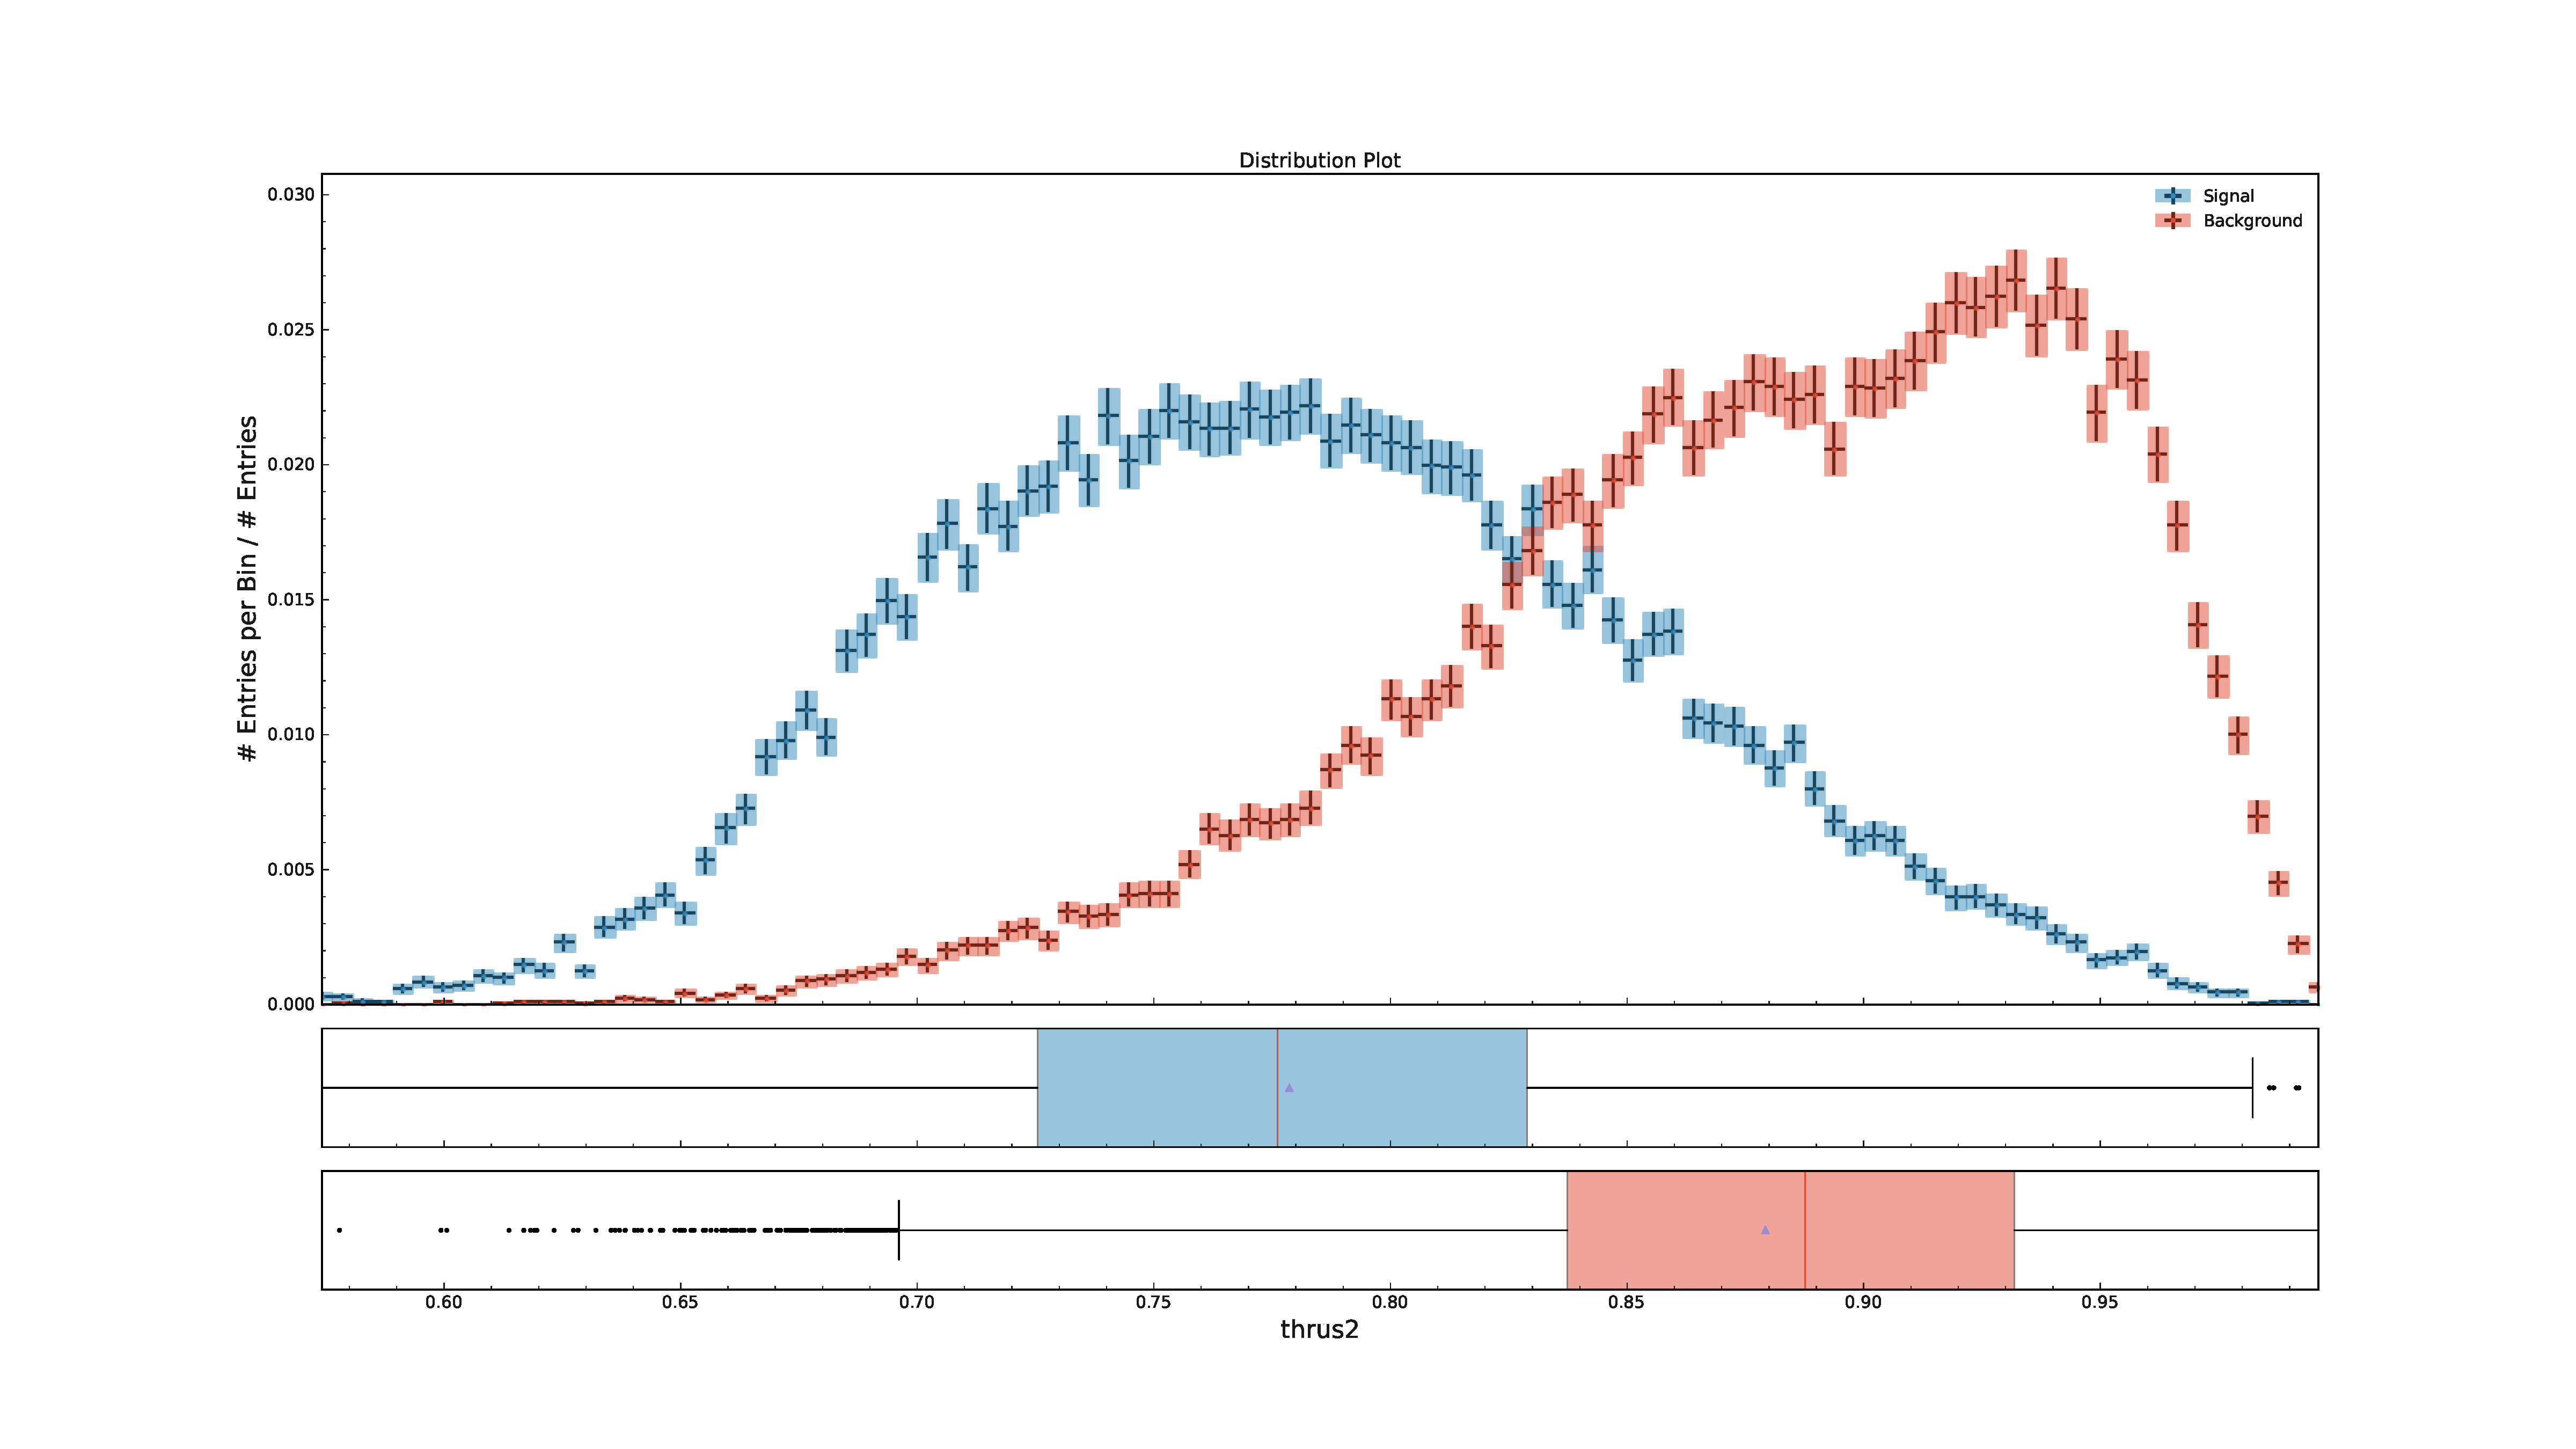
\includegraphics[width=1.0\textwidth]{variable_-5586688839139693641.pdf}
\end{center}
\subsection{cosTBTO}
\begin{center}
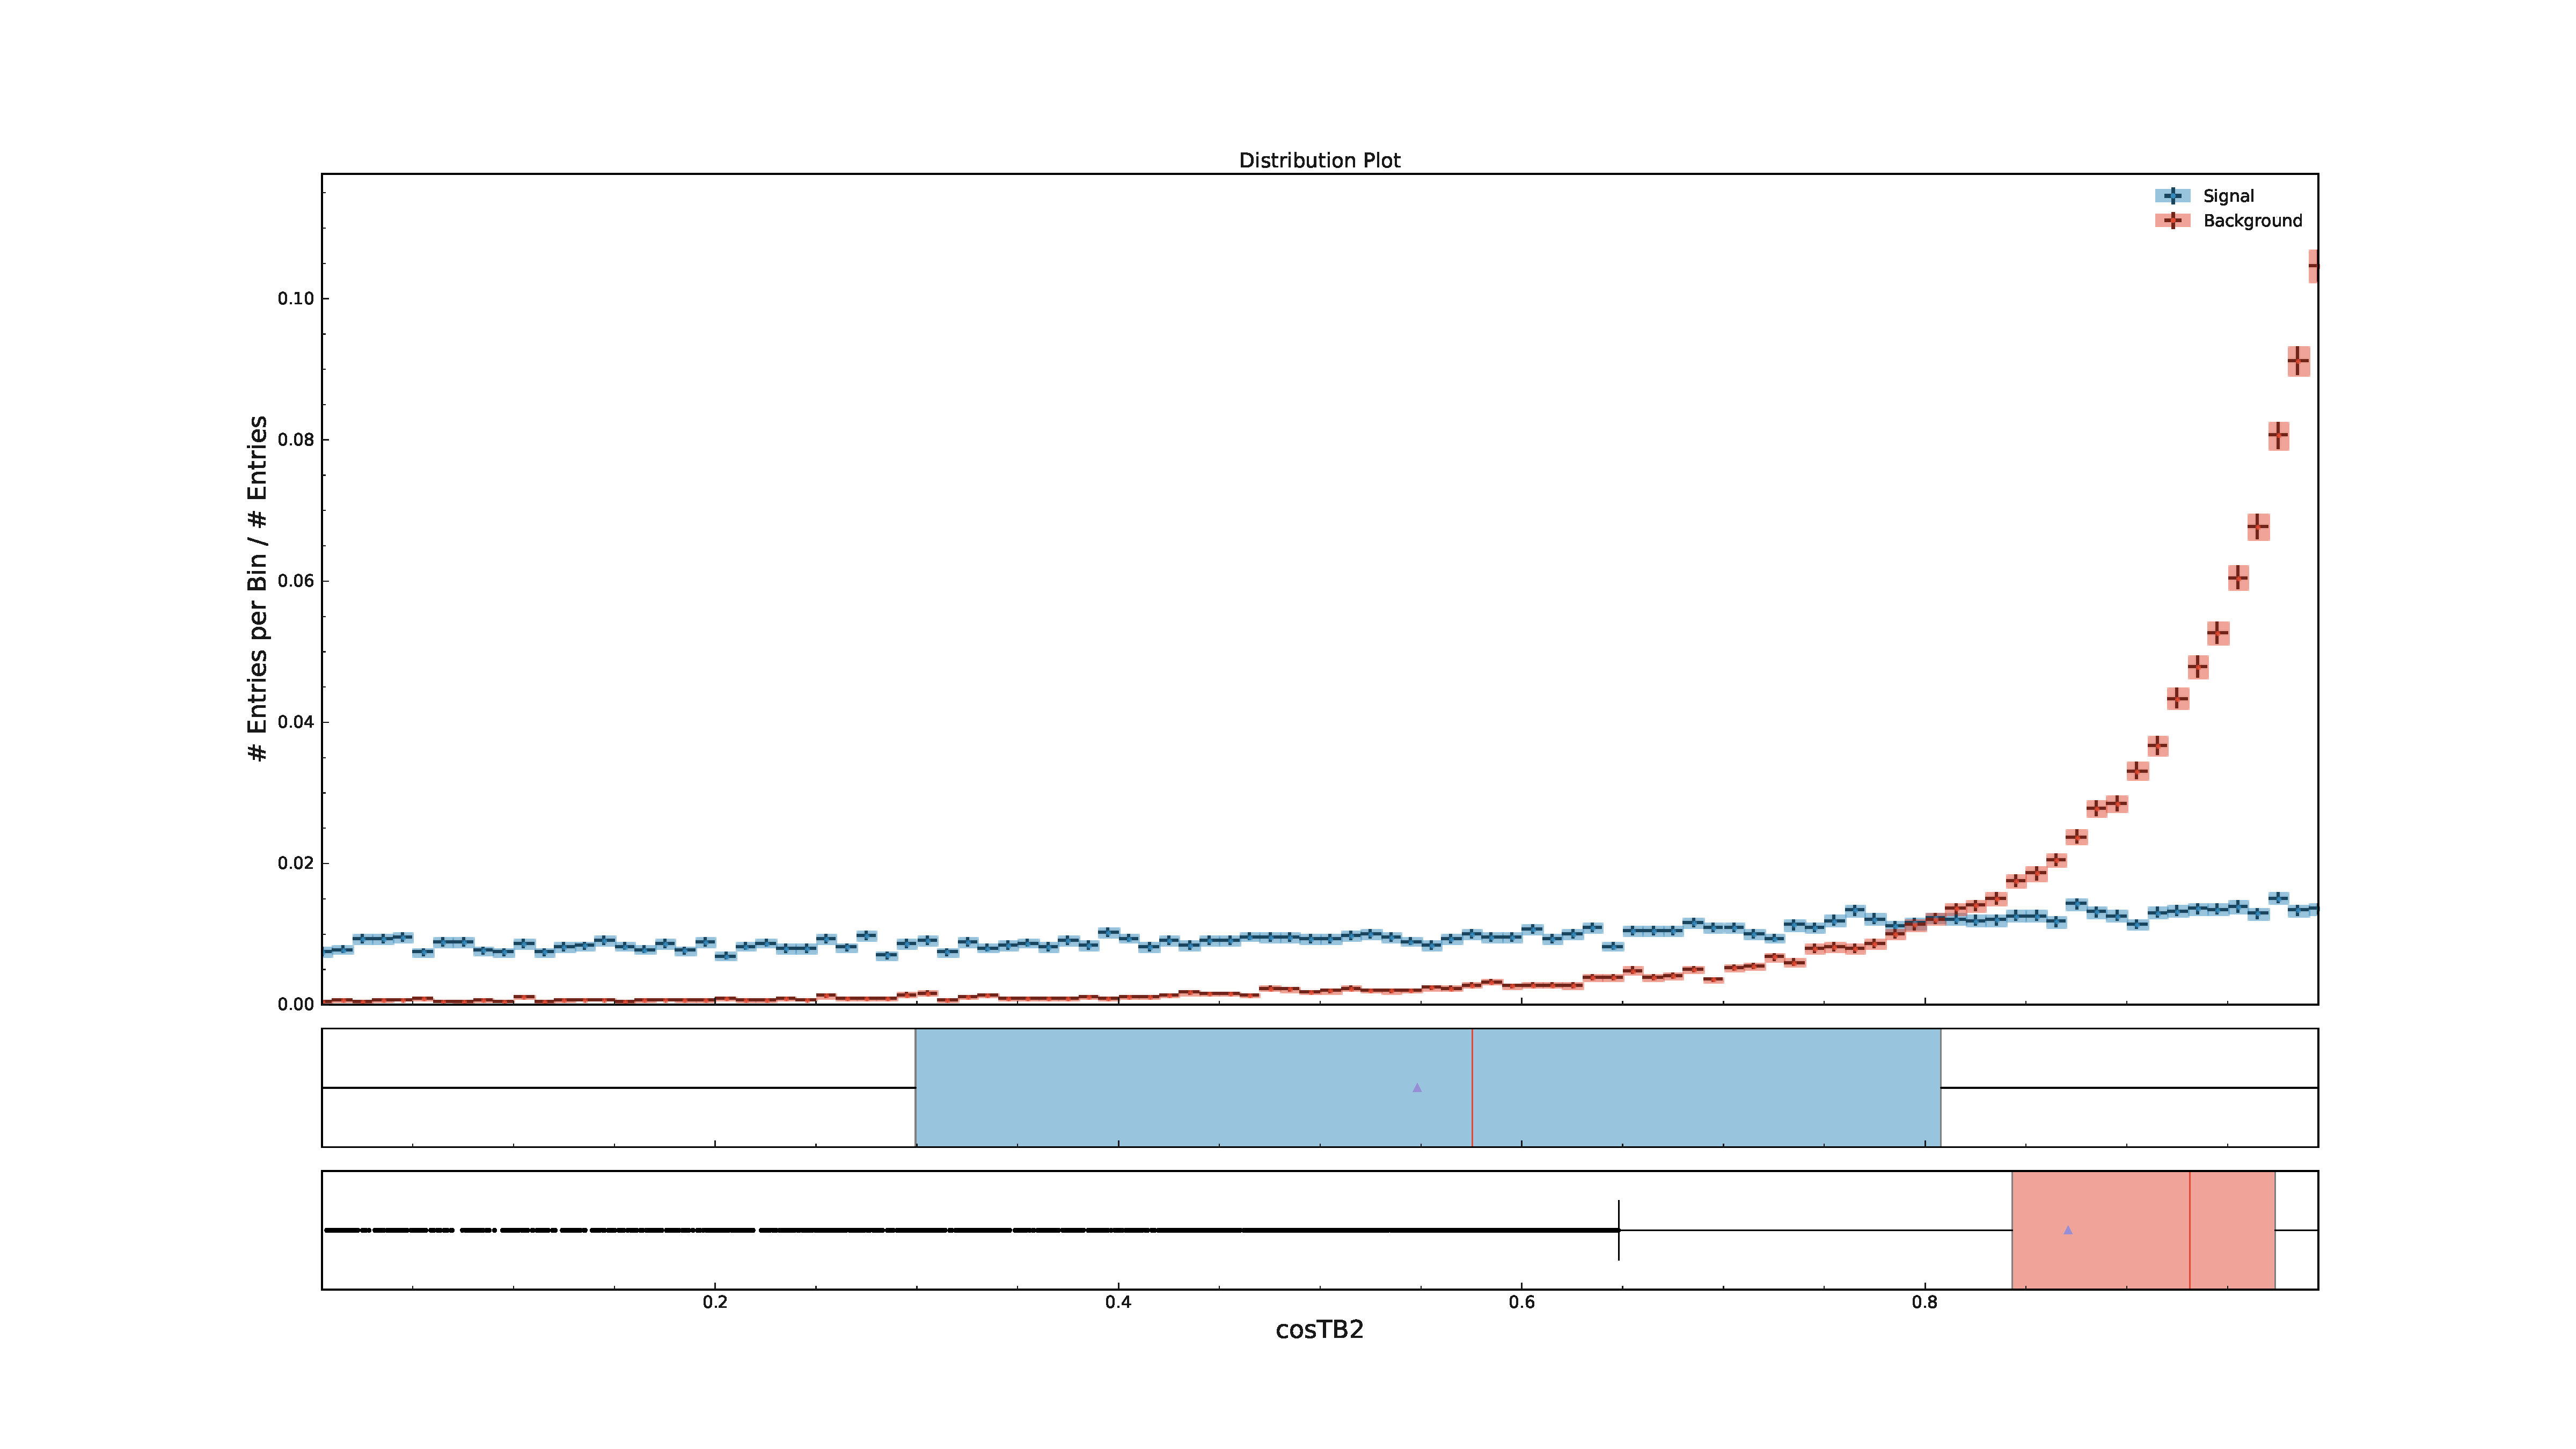
\includegraphics[width=1.0\textwidth]{variable_-448030578511342677.pdf}
\end{center}
\subsection{abs\_qr}
\begin{center}
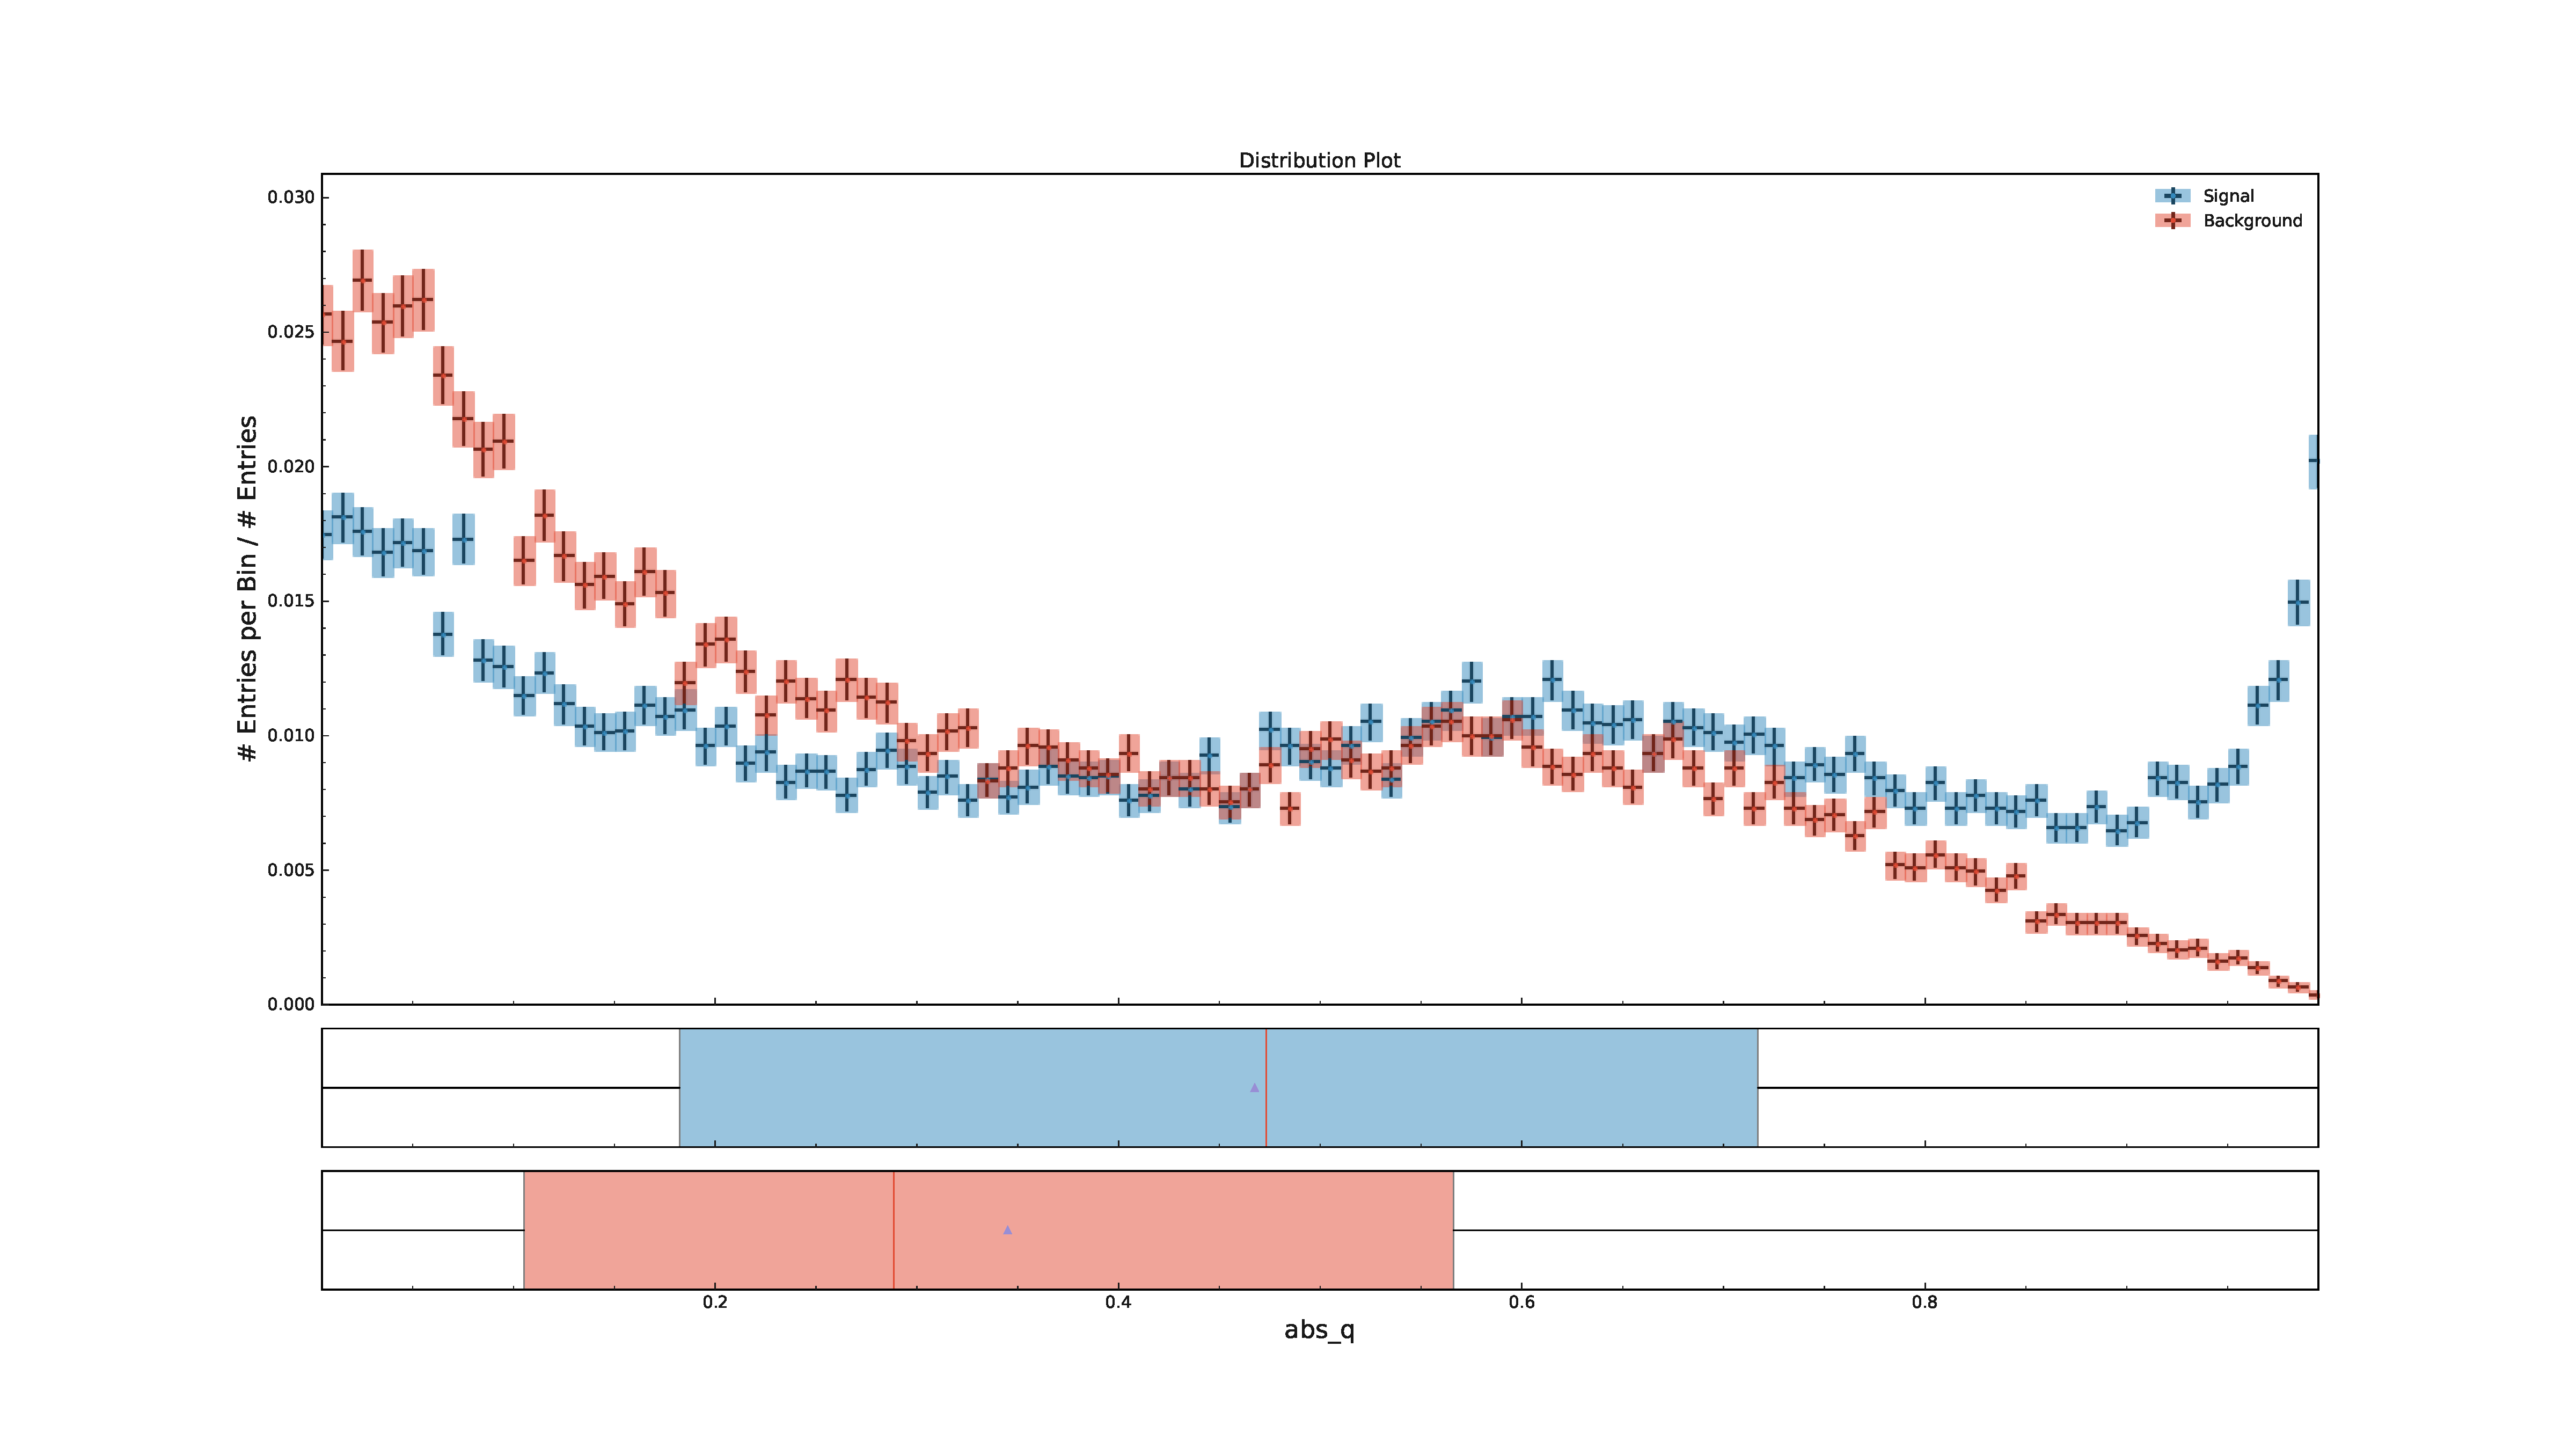
\includegraphics[width=1.0\textwidth]{variable_7565637163324965417.pdf}
\end{center}
\subsection{DeltaZ}
\begin{center}
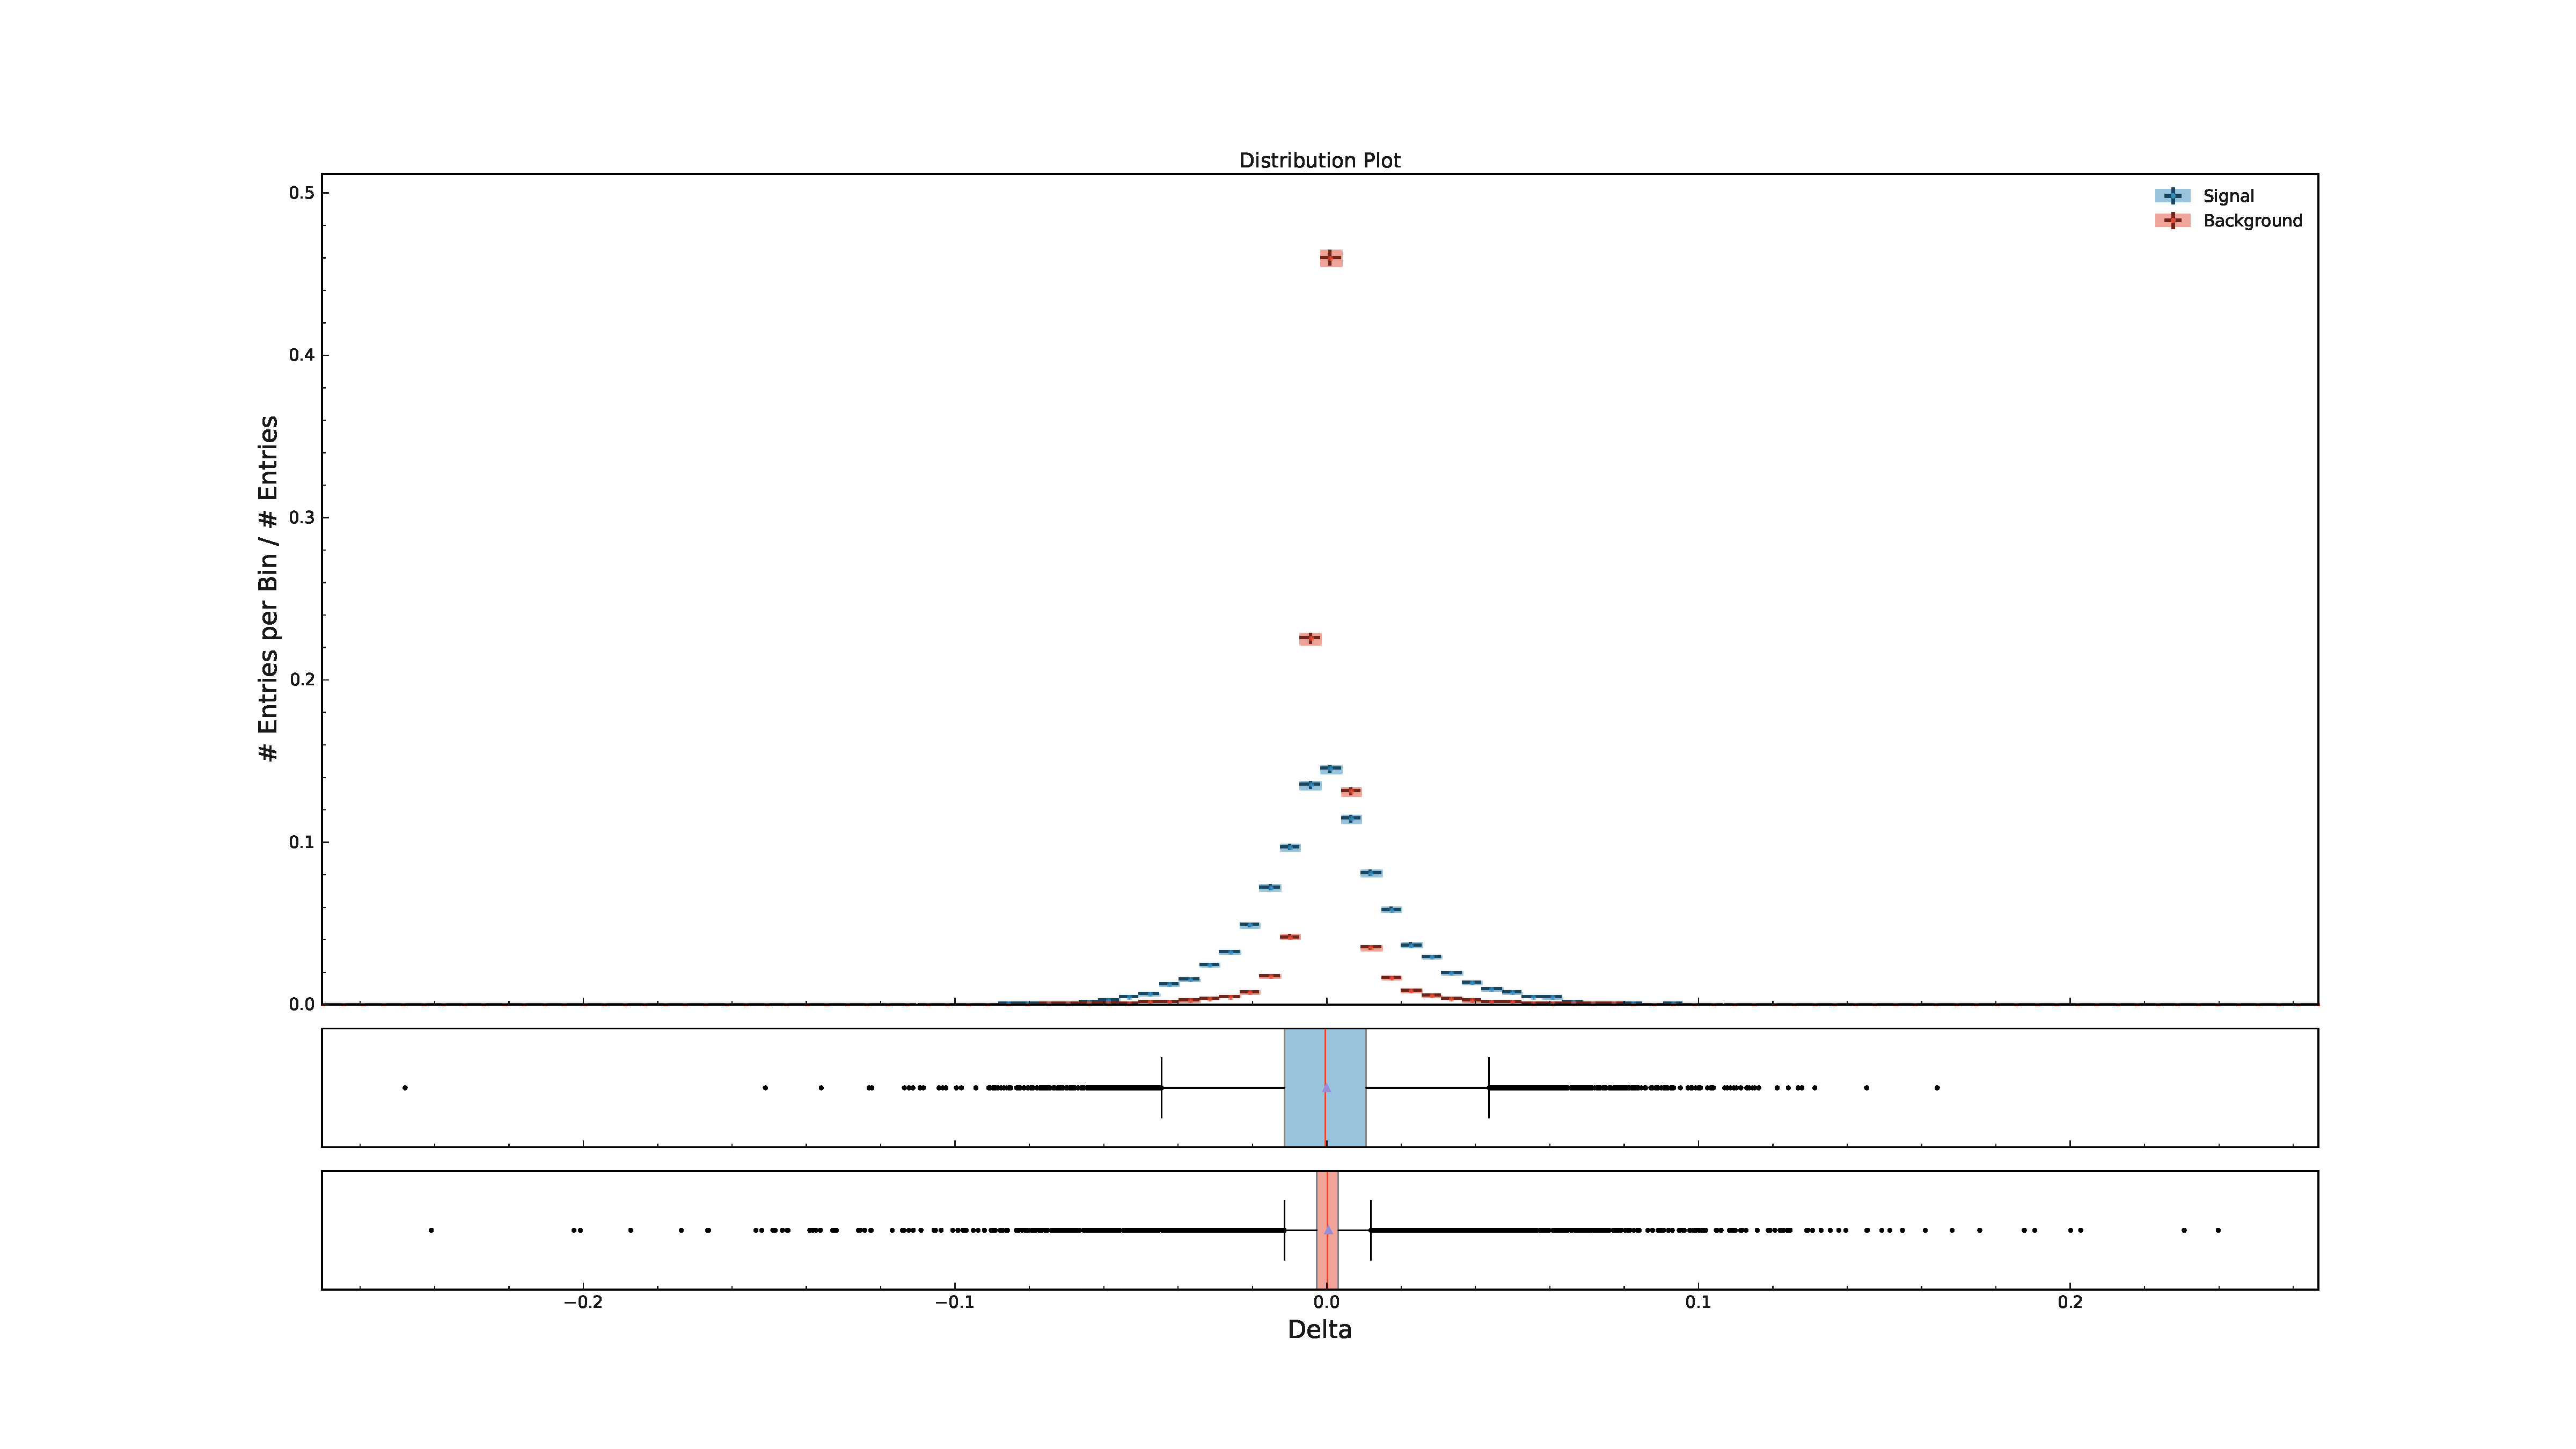
\includegraphics[width=1.0\textwidth]{variable_-6872944916743380479.pdf}
\end{center}
\subsection{R2}
\begin{center}
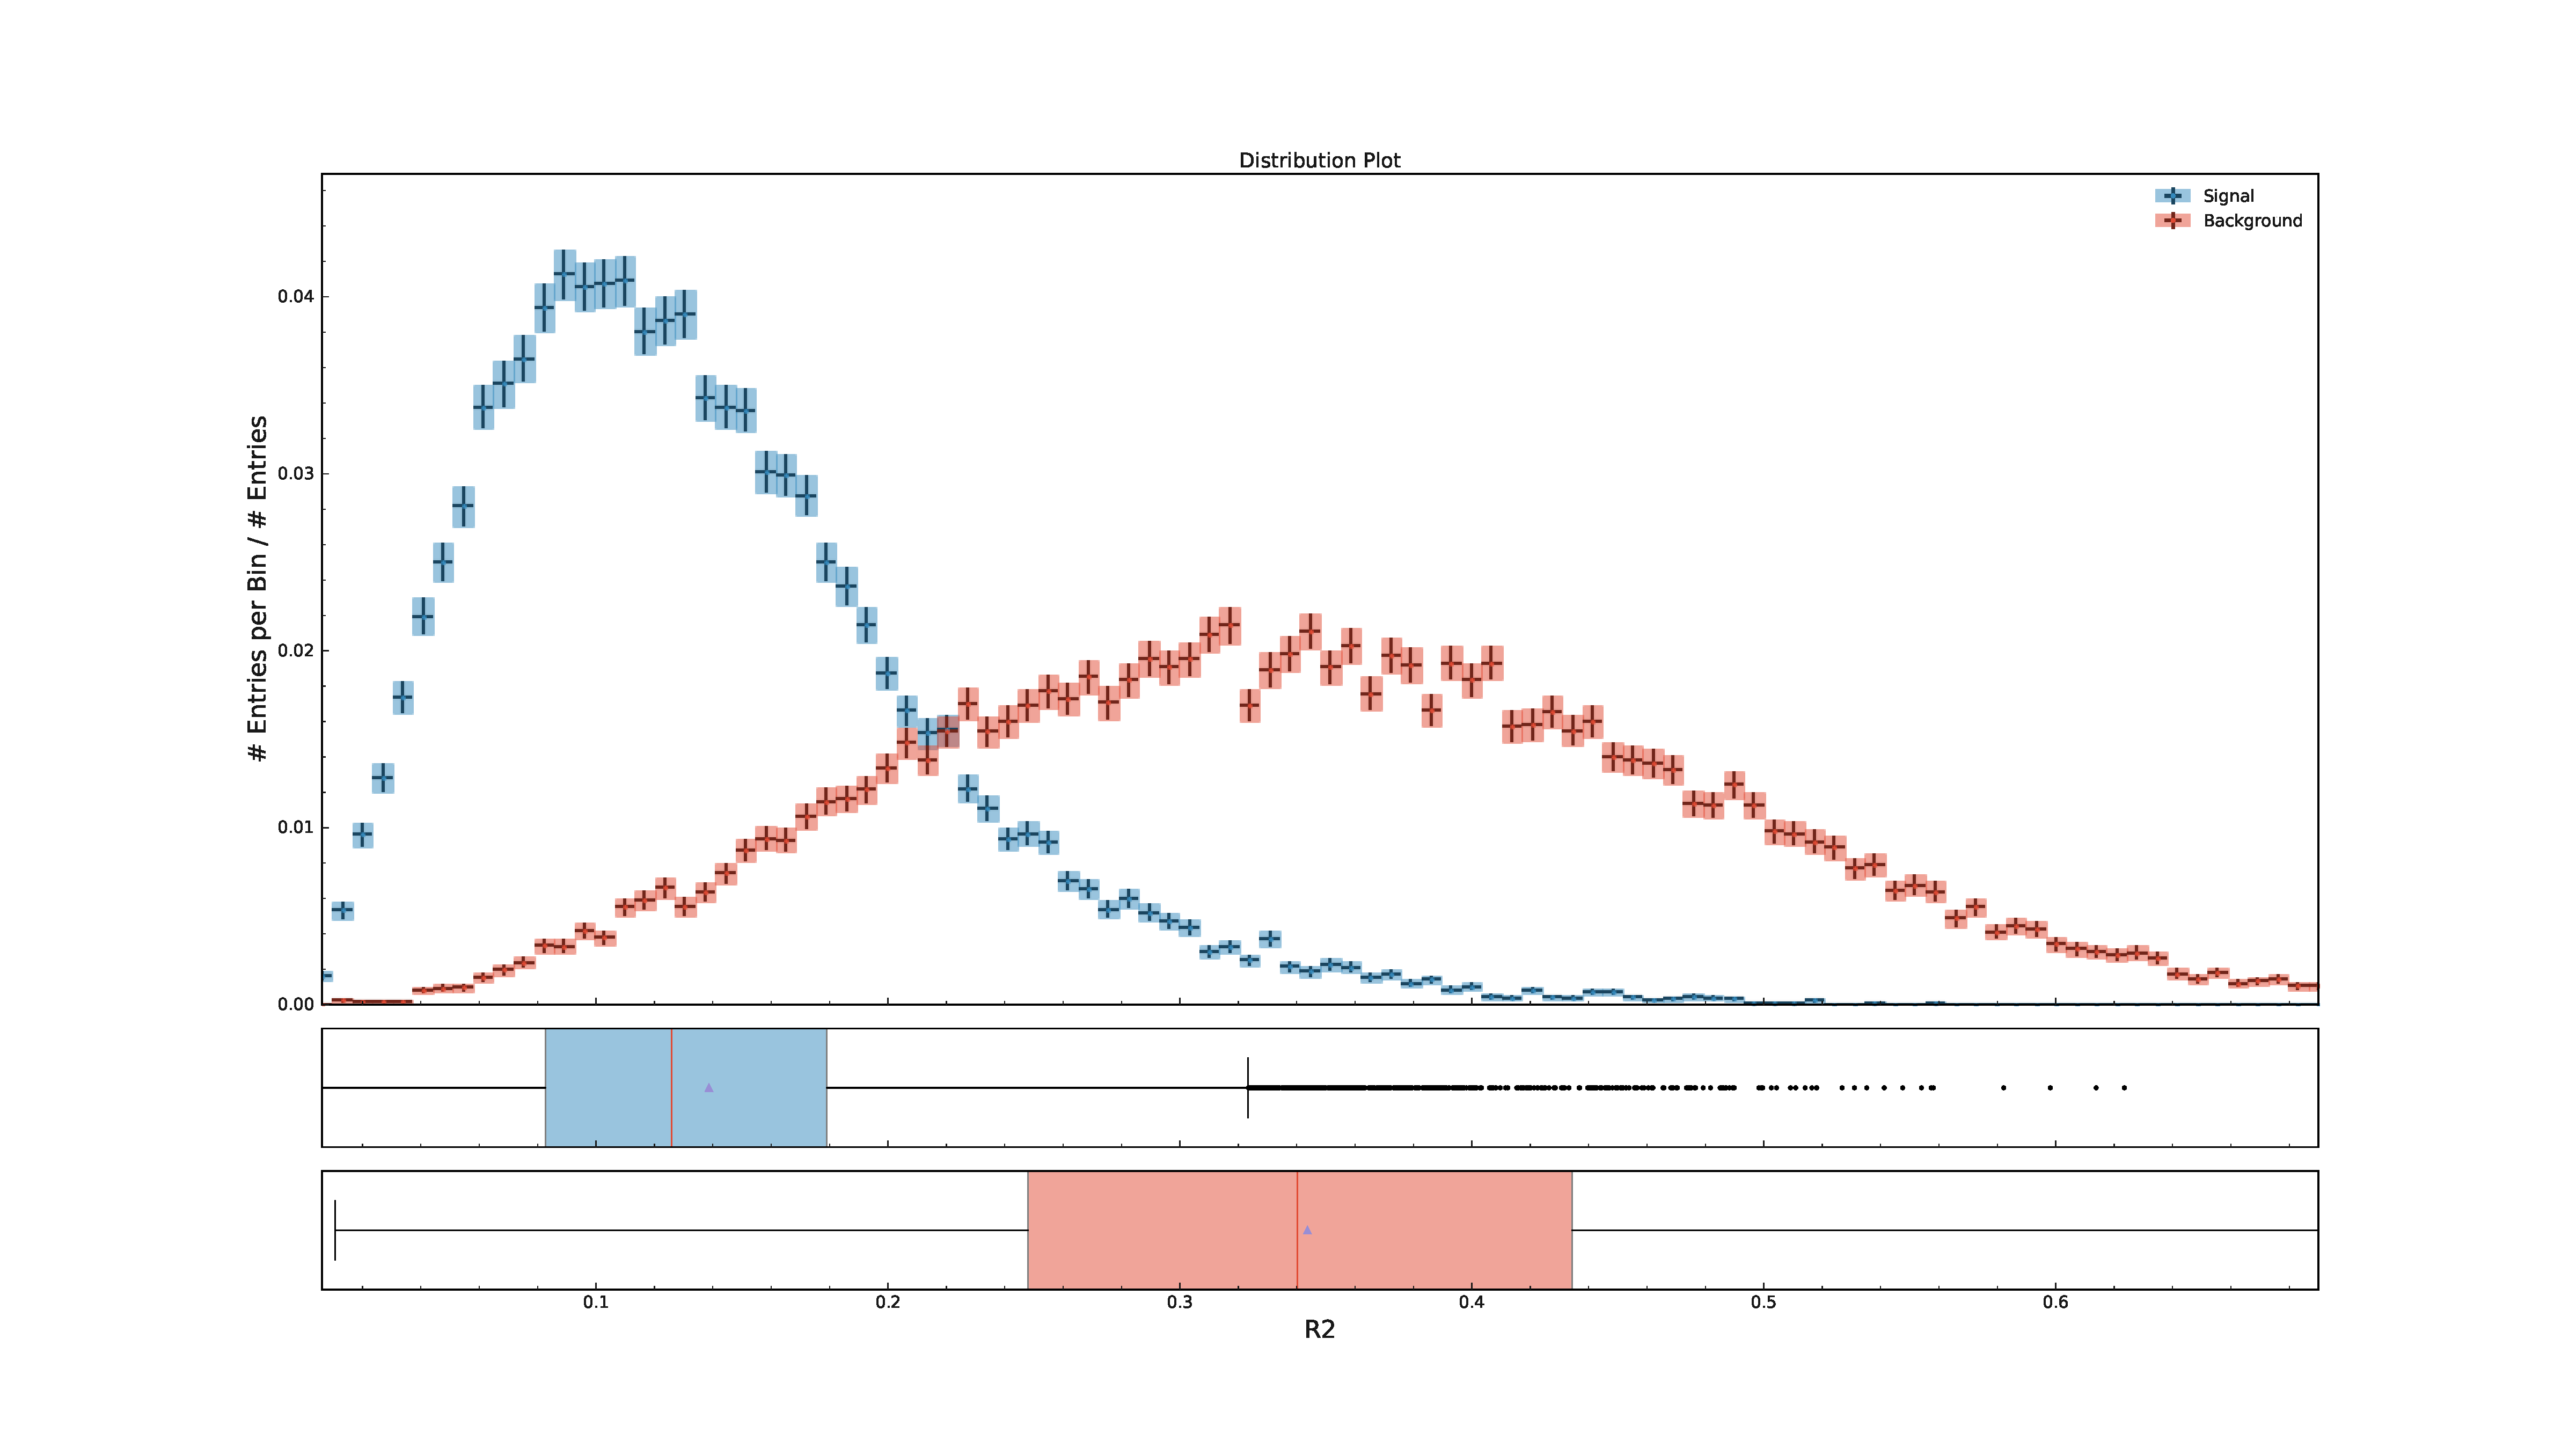
\includegraphics[width=1.0\textwidth]{variable_7345058823840298118.pdf}
\end{center}
\raggedbottom
\pagebreak[0]
\FloatBarrier
\section{Classifier Plot}
This section contains the receiver operating characteristics (ROC), purity projection, ...of the classifiers on training and independent data.The legend of each plot contains the shortened identifier and the area under the ROC curvein parenthesis.\raggedbottom
\pagebreak[0]
\FloatBarrier
\section{ROC Plot}
\begin{center}
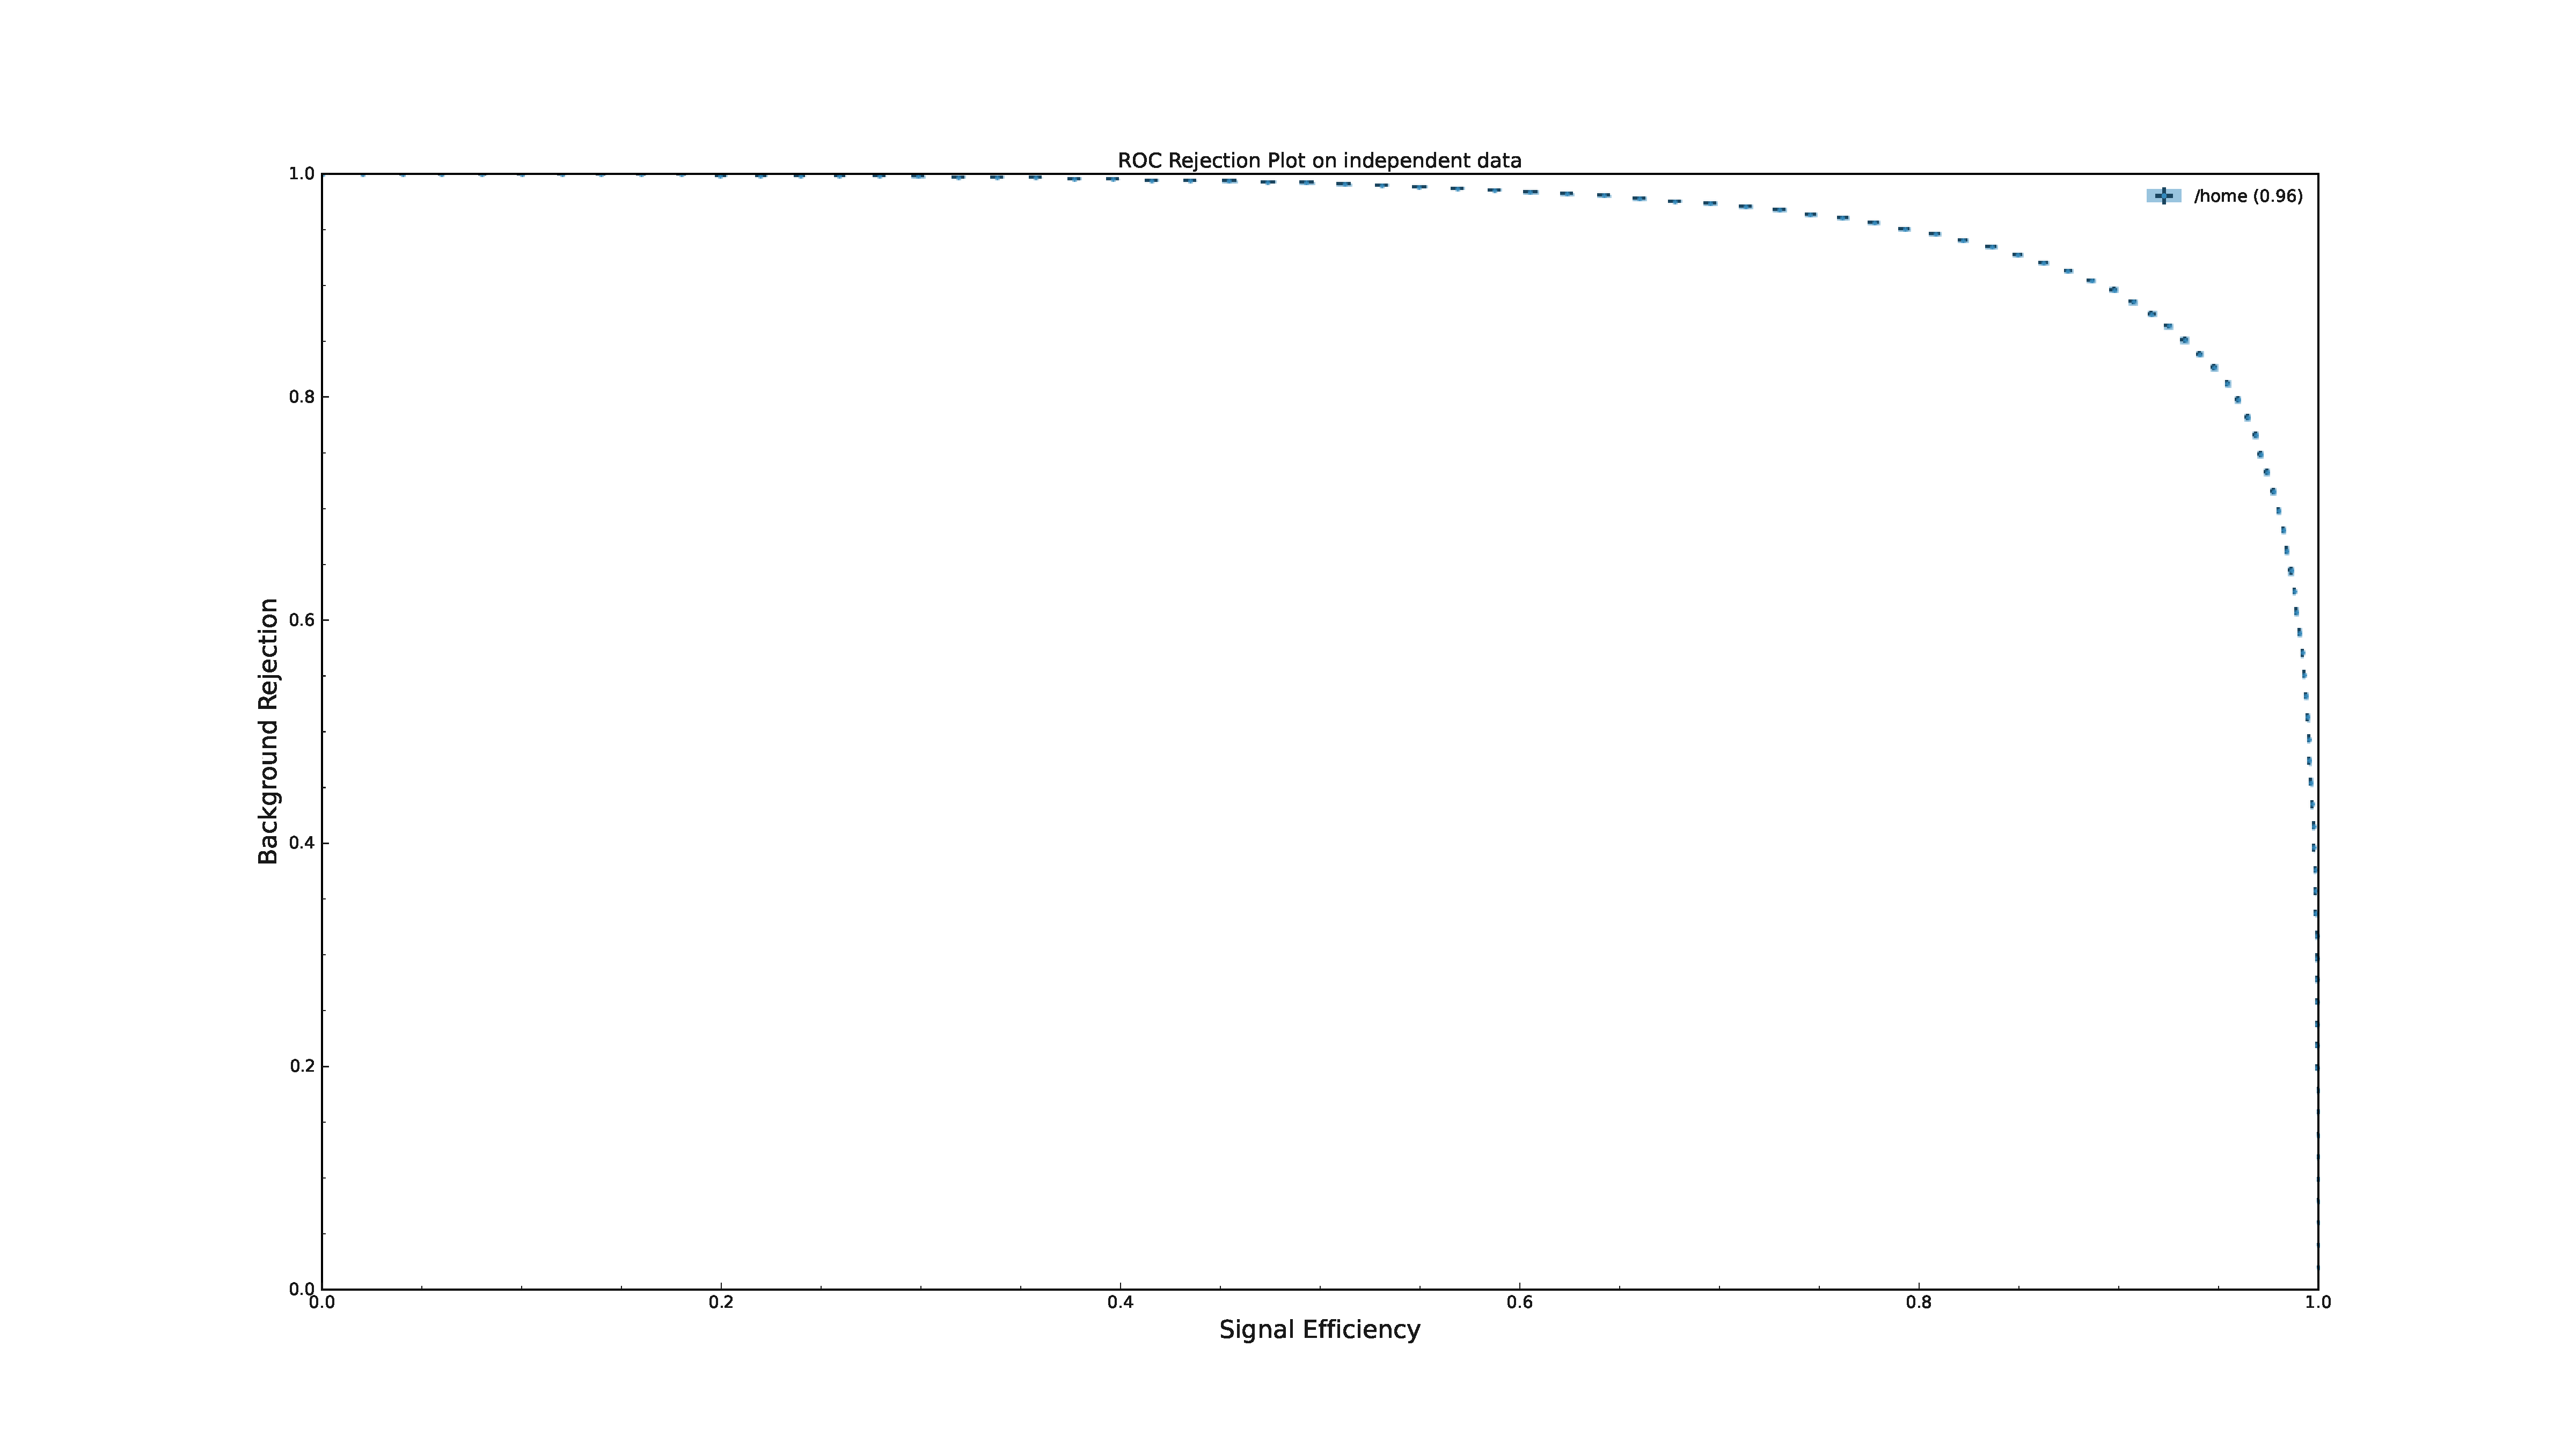
\includegraphics[width=1.0\textwidth]{roc_plot_test.pdf}
\end{center}
\begin{center}
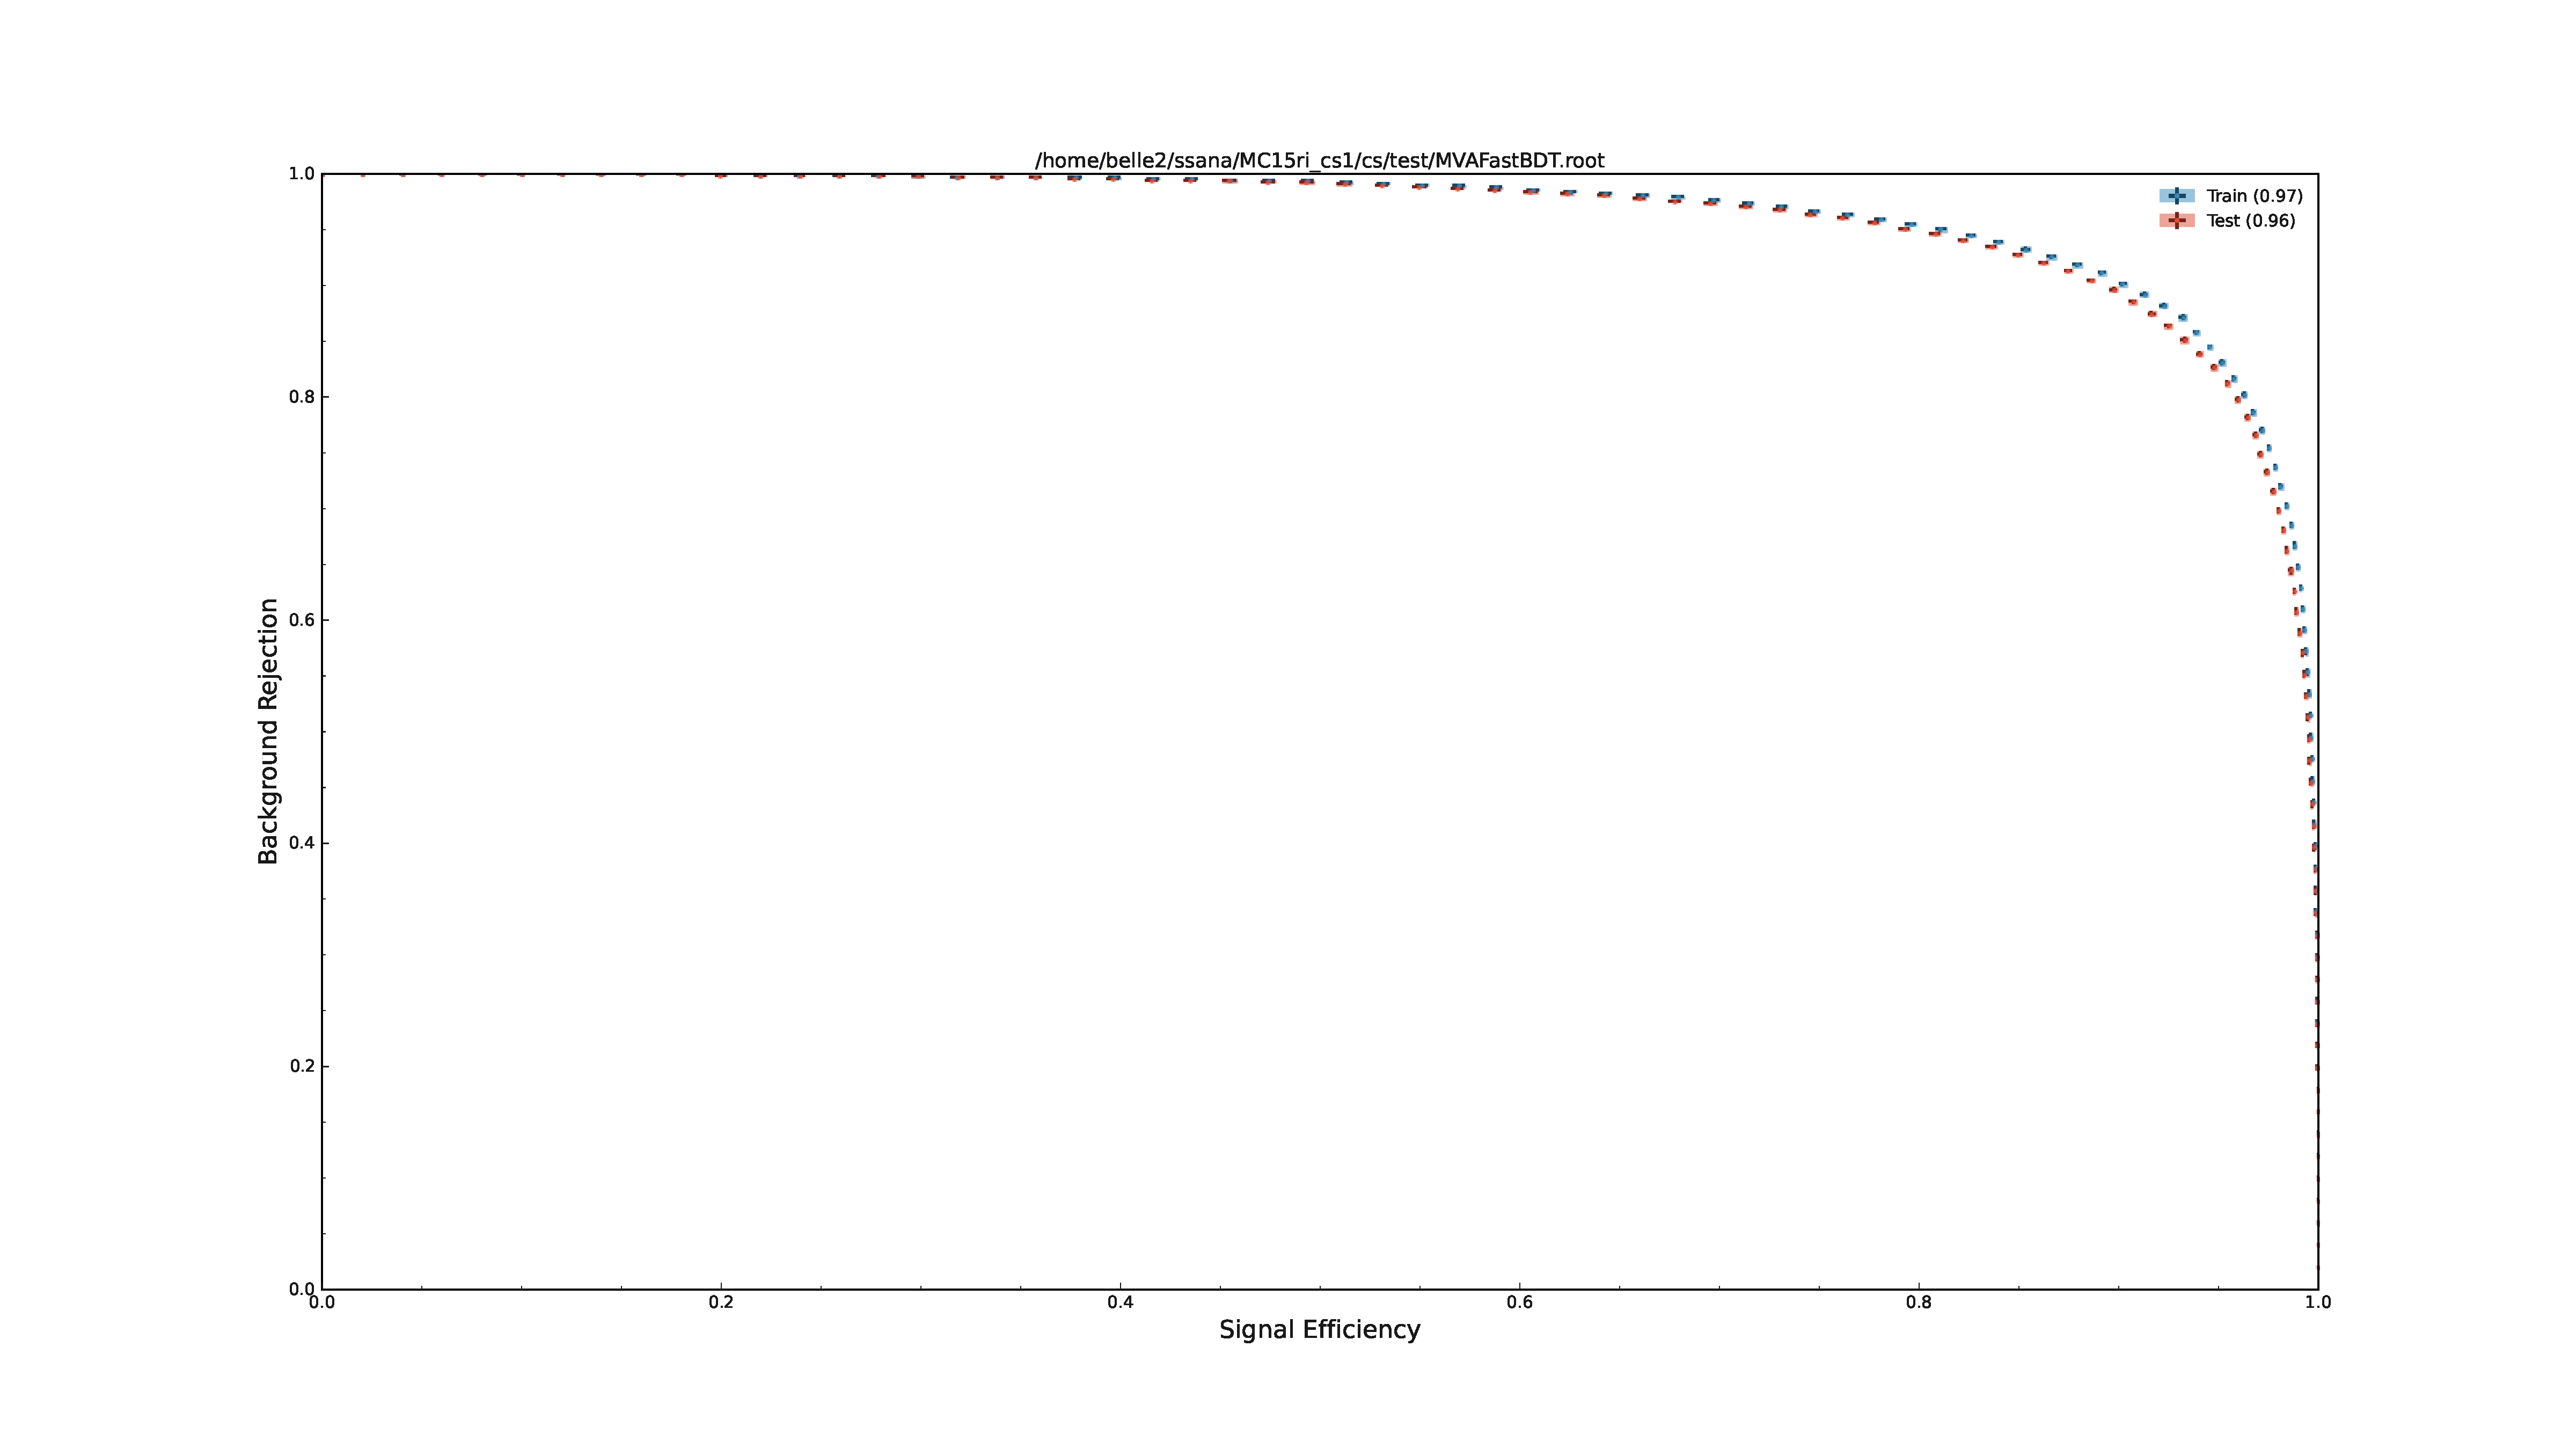
\includegraphics[width=1.0\textwidth]{roc_test_-936217630058450507.pdf}
\end{center}
\raggedbottom
\pagebreak[0]
\FloatBarrier
\section{Classification Results}
\subsection{/home}
\begin{center}
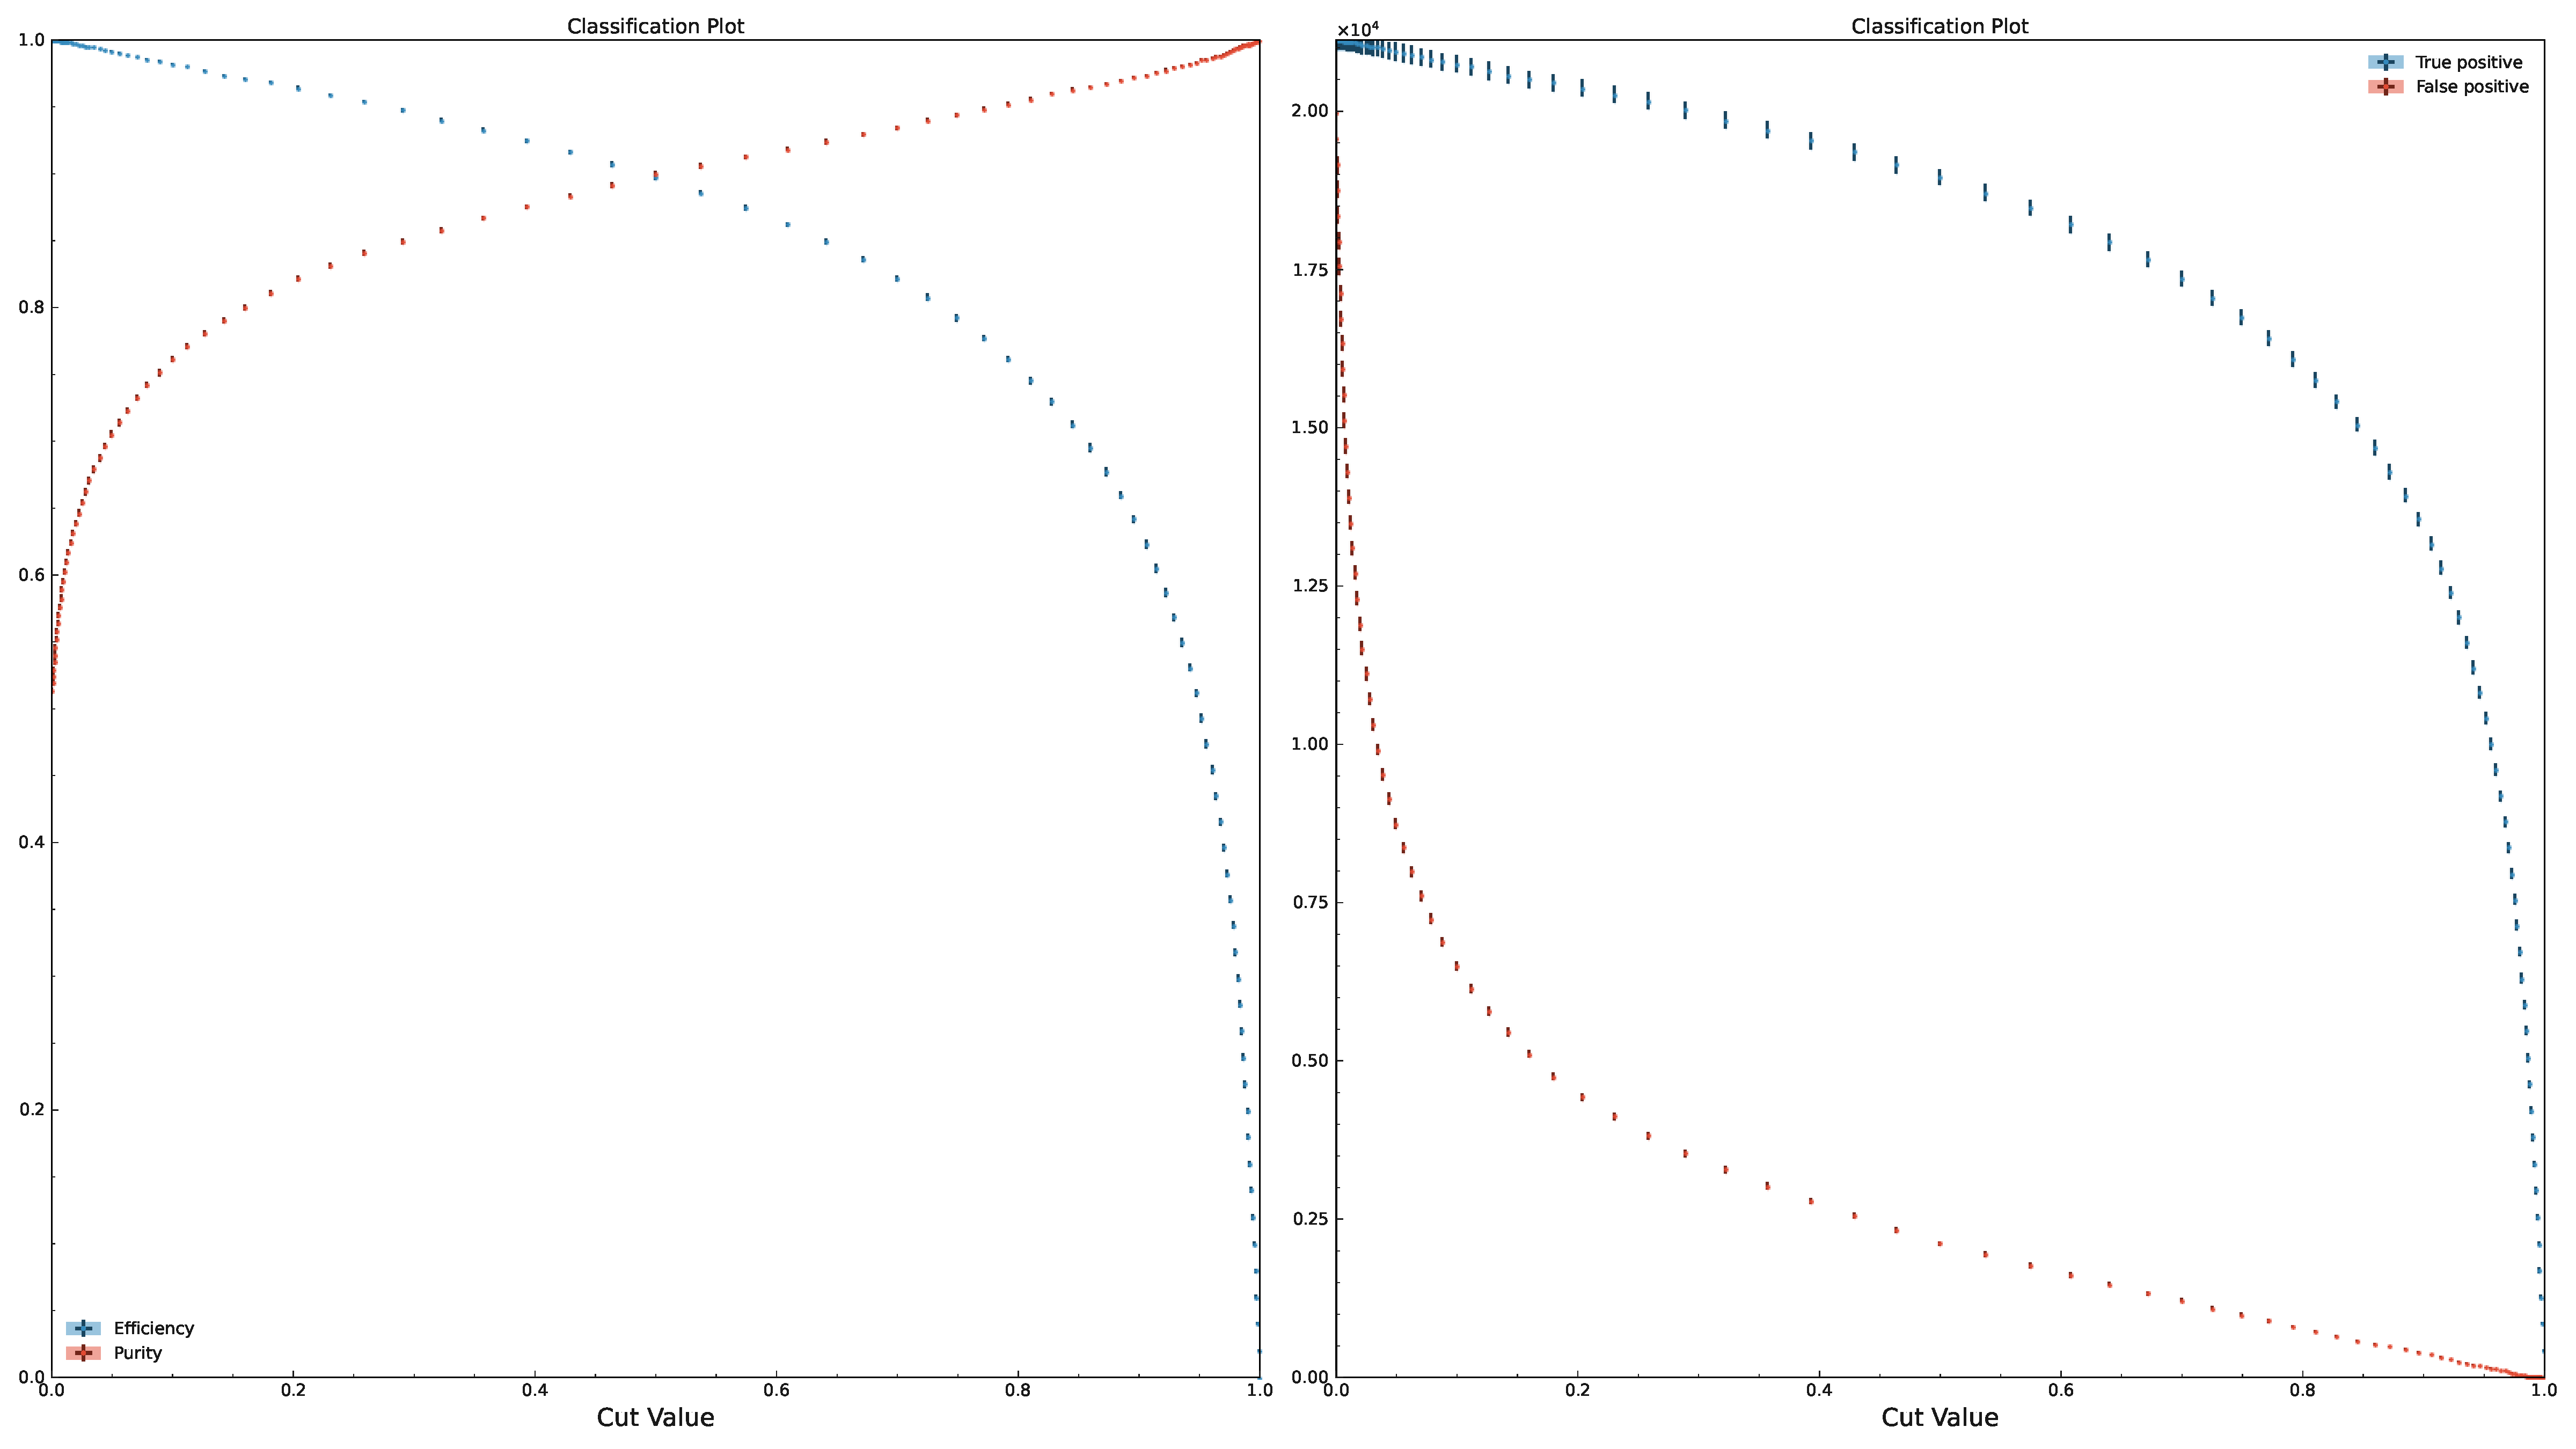
\includegraphics[width=1\textwidth]{classification_result_-936217630058450507.pdf}
\end{center}
\raggedbottom
\pagebreak[0]
\FloatBarrier
\section{Diagonal Plot}
\subsection{/home}
\begin{center}
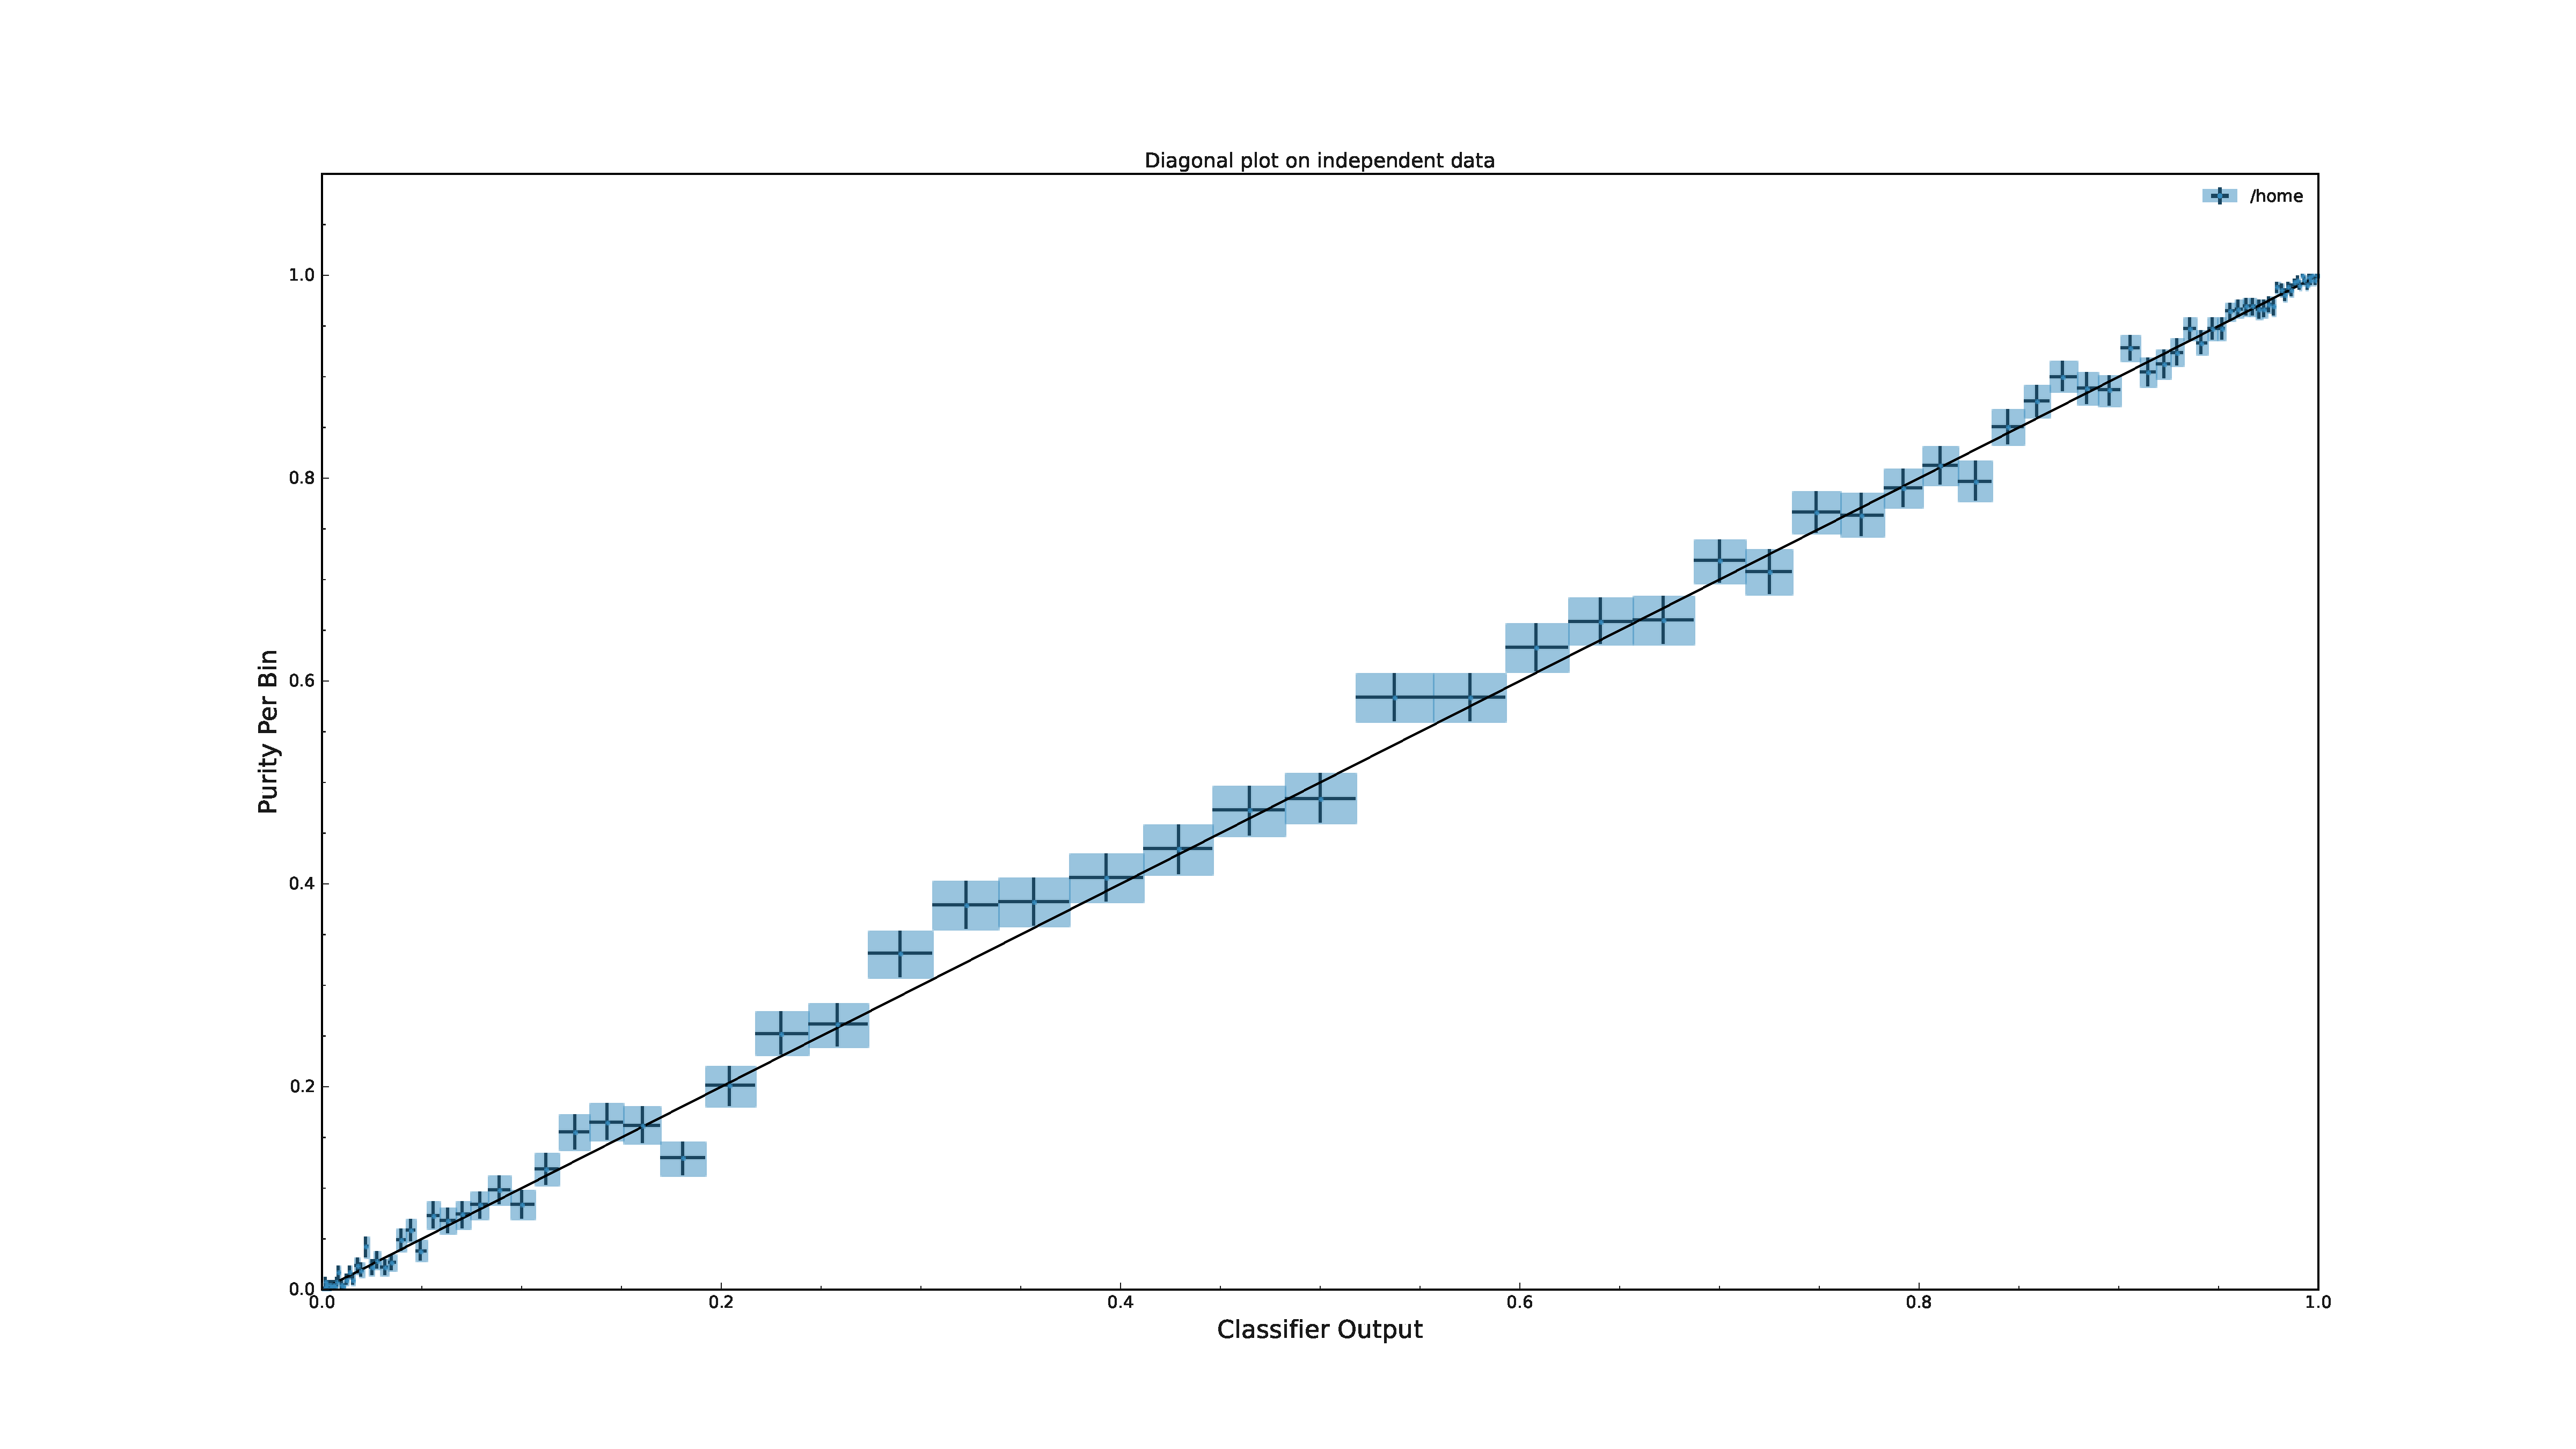
\includegraphics[width=1.0\textwidth]{diagonal_plot_test.pdf}
\end{center}
\subsection{Overtraining Plot}
\begin{center}
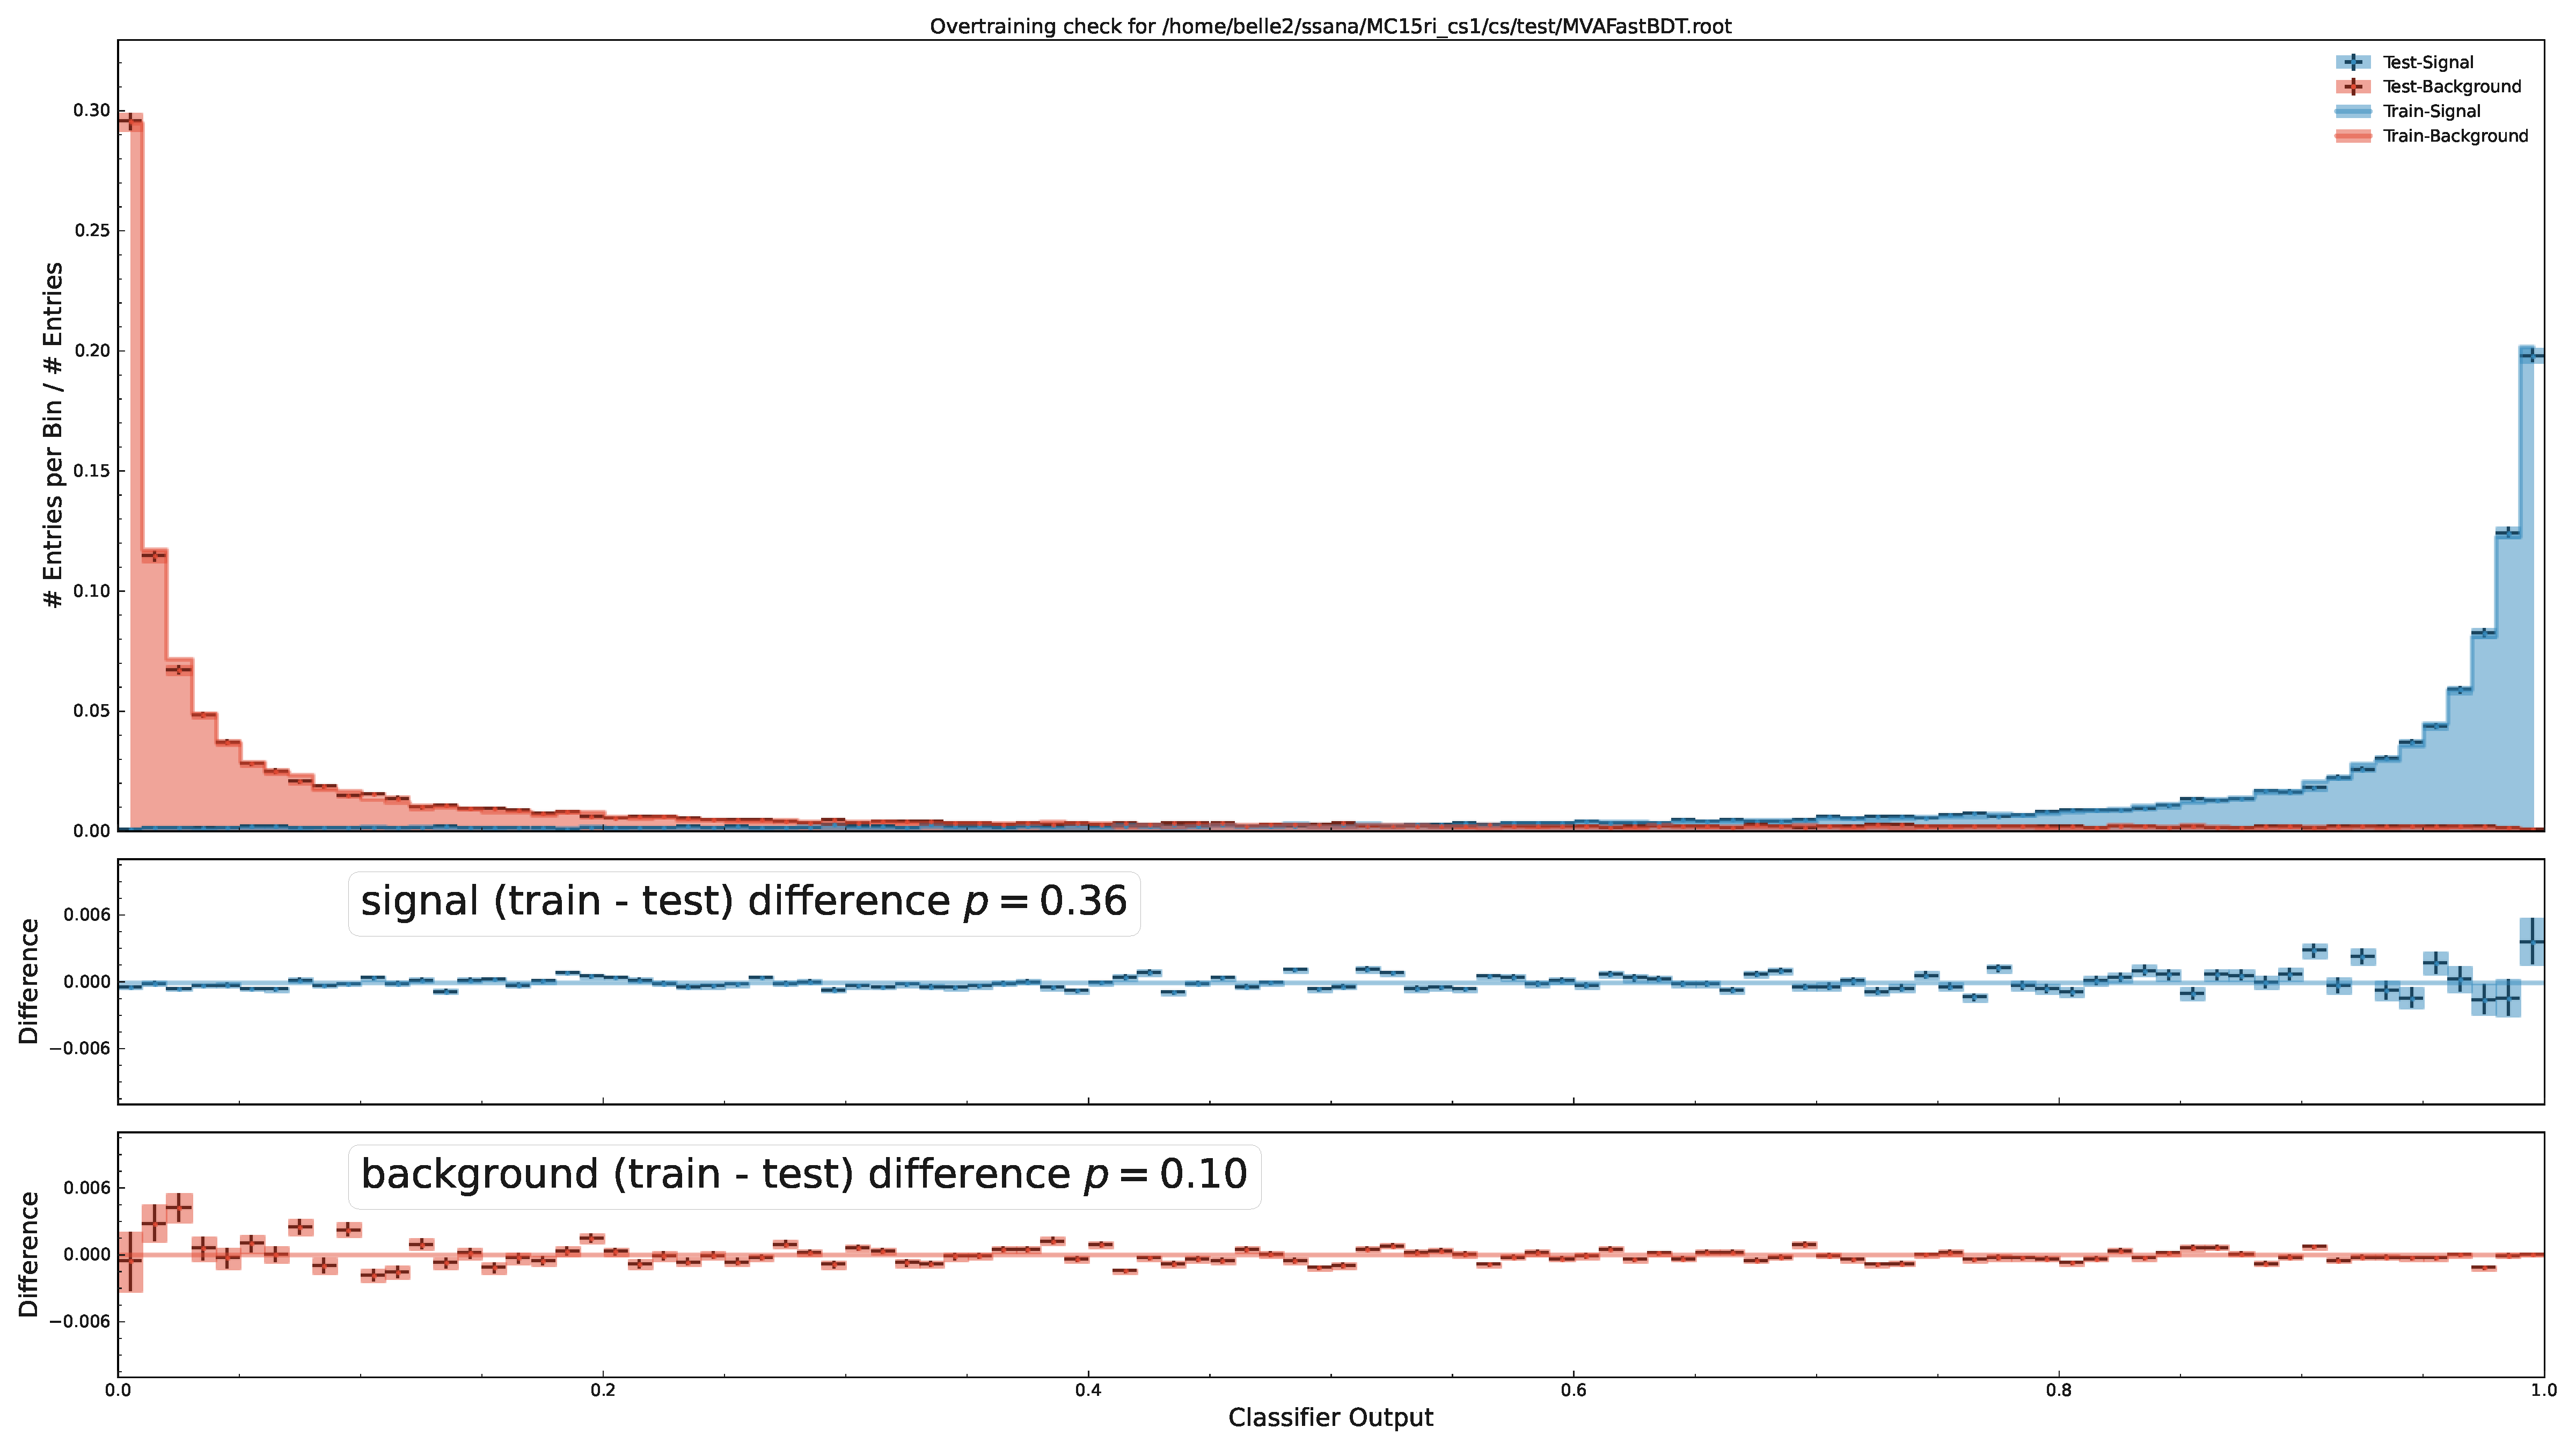
\includegraphics[width=1.0\textwidth]{overtraining_plot_-936217630058450507.pdf}
\end{center}
\raggedbottom
\pagebreak[0]
\FloatBarrier
\section{Spectators}
This section contains the distribution and dependence on theclassifier outputs of all spectator variables.\begin{center}
\begin{longtable}{ll}
\caption{Abbreviations of spectators}\\
\toprule
Spectator & Abbreviation\\
\midrule
\bottomrule
\end{longtable}
\end{center}
\end{document}